%
%
% (c) 2020 Michael Schmid, Hochschule Rapperswil
%
% !TEX root = ../presentation.tex

\begin{frame}
  \frametitle{Explicit Euler Method}
  How to rewrtie our PDE?
  $$ \frac {\partial u}{\partial t}+u{\frac {\partial u}{\partial x}}=0 $$

\end{frame}



\begin{frame}
  \begin{columns}
    \column{0.5\linewidth}
    Euler forwards
  $$\frac{u_{i}^{n}-u_{i}^{n-1}}{\Delta t}+ u_{i}^{n}\, \frac{u_{i}^{n-1}-u_{i-1}^{n-1}}{\Delta x}=0$$
  $$ u_{i}^{n} = \frac{\Delta{x}\, u^{n-1}_{i}\,}{- \Delta{t}\, u^{n-1}_{i-1}\, + \Delta{t}\, u^{n-1}_{i}\, + \Delta{x}\,}$$
    \column{0.5\linewidth}
    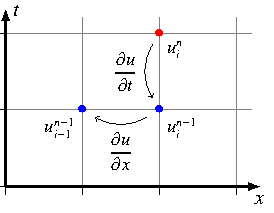
\includegraphics[width=\linewidth]{../BurgersEquation/tikz/linear1/linear1.pdf}\\
  \end{columns}
\end{frame}

\begin{frame}
  \begin{columns}
    \column{0.5\linewidth}
    Euler forwards

  $$\frac{u_{i}^{n}-u_{i}^{n-1}}{\Delta t}+ u_{i}^{n-1}\, \frac{u_{i}^{n-1}-u_{i-1}^{n-1}}{\Delta x}=0$$
  $$ u_{i}^{n} = \frac{u^{n-1}_{i}\, \left(\Delta{t}\, u^{n-1}_{i-1}\, - \Delta{t}\, u^{n-1}_{i}\, + \Delta{x}\,\right)}{\Delta{x}\,}$$
    \column{0.5\linewidth}
    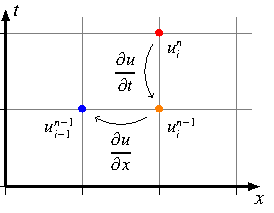
\includegraphics[width=\linewidth]{../BurgersEquation/tikz/linear2/linear2.pdf}\\
  \end{columns}
\end{frame}

\begin{frame}
  \frametitle{convergence condition by Courant–Friedrichs–Lewy}
  \Huge{
  $$ c = \frac{u \, \Delta t}{\Delta x} < 1  $$
}
\end{frame}

% \begin{frame}
%   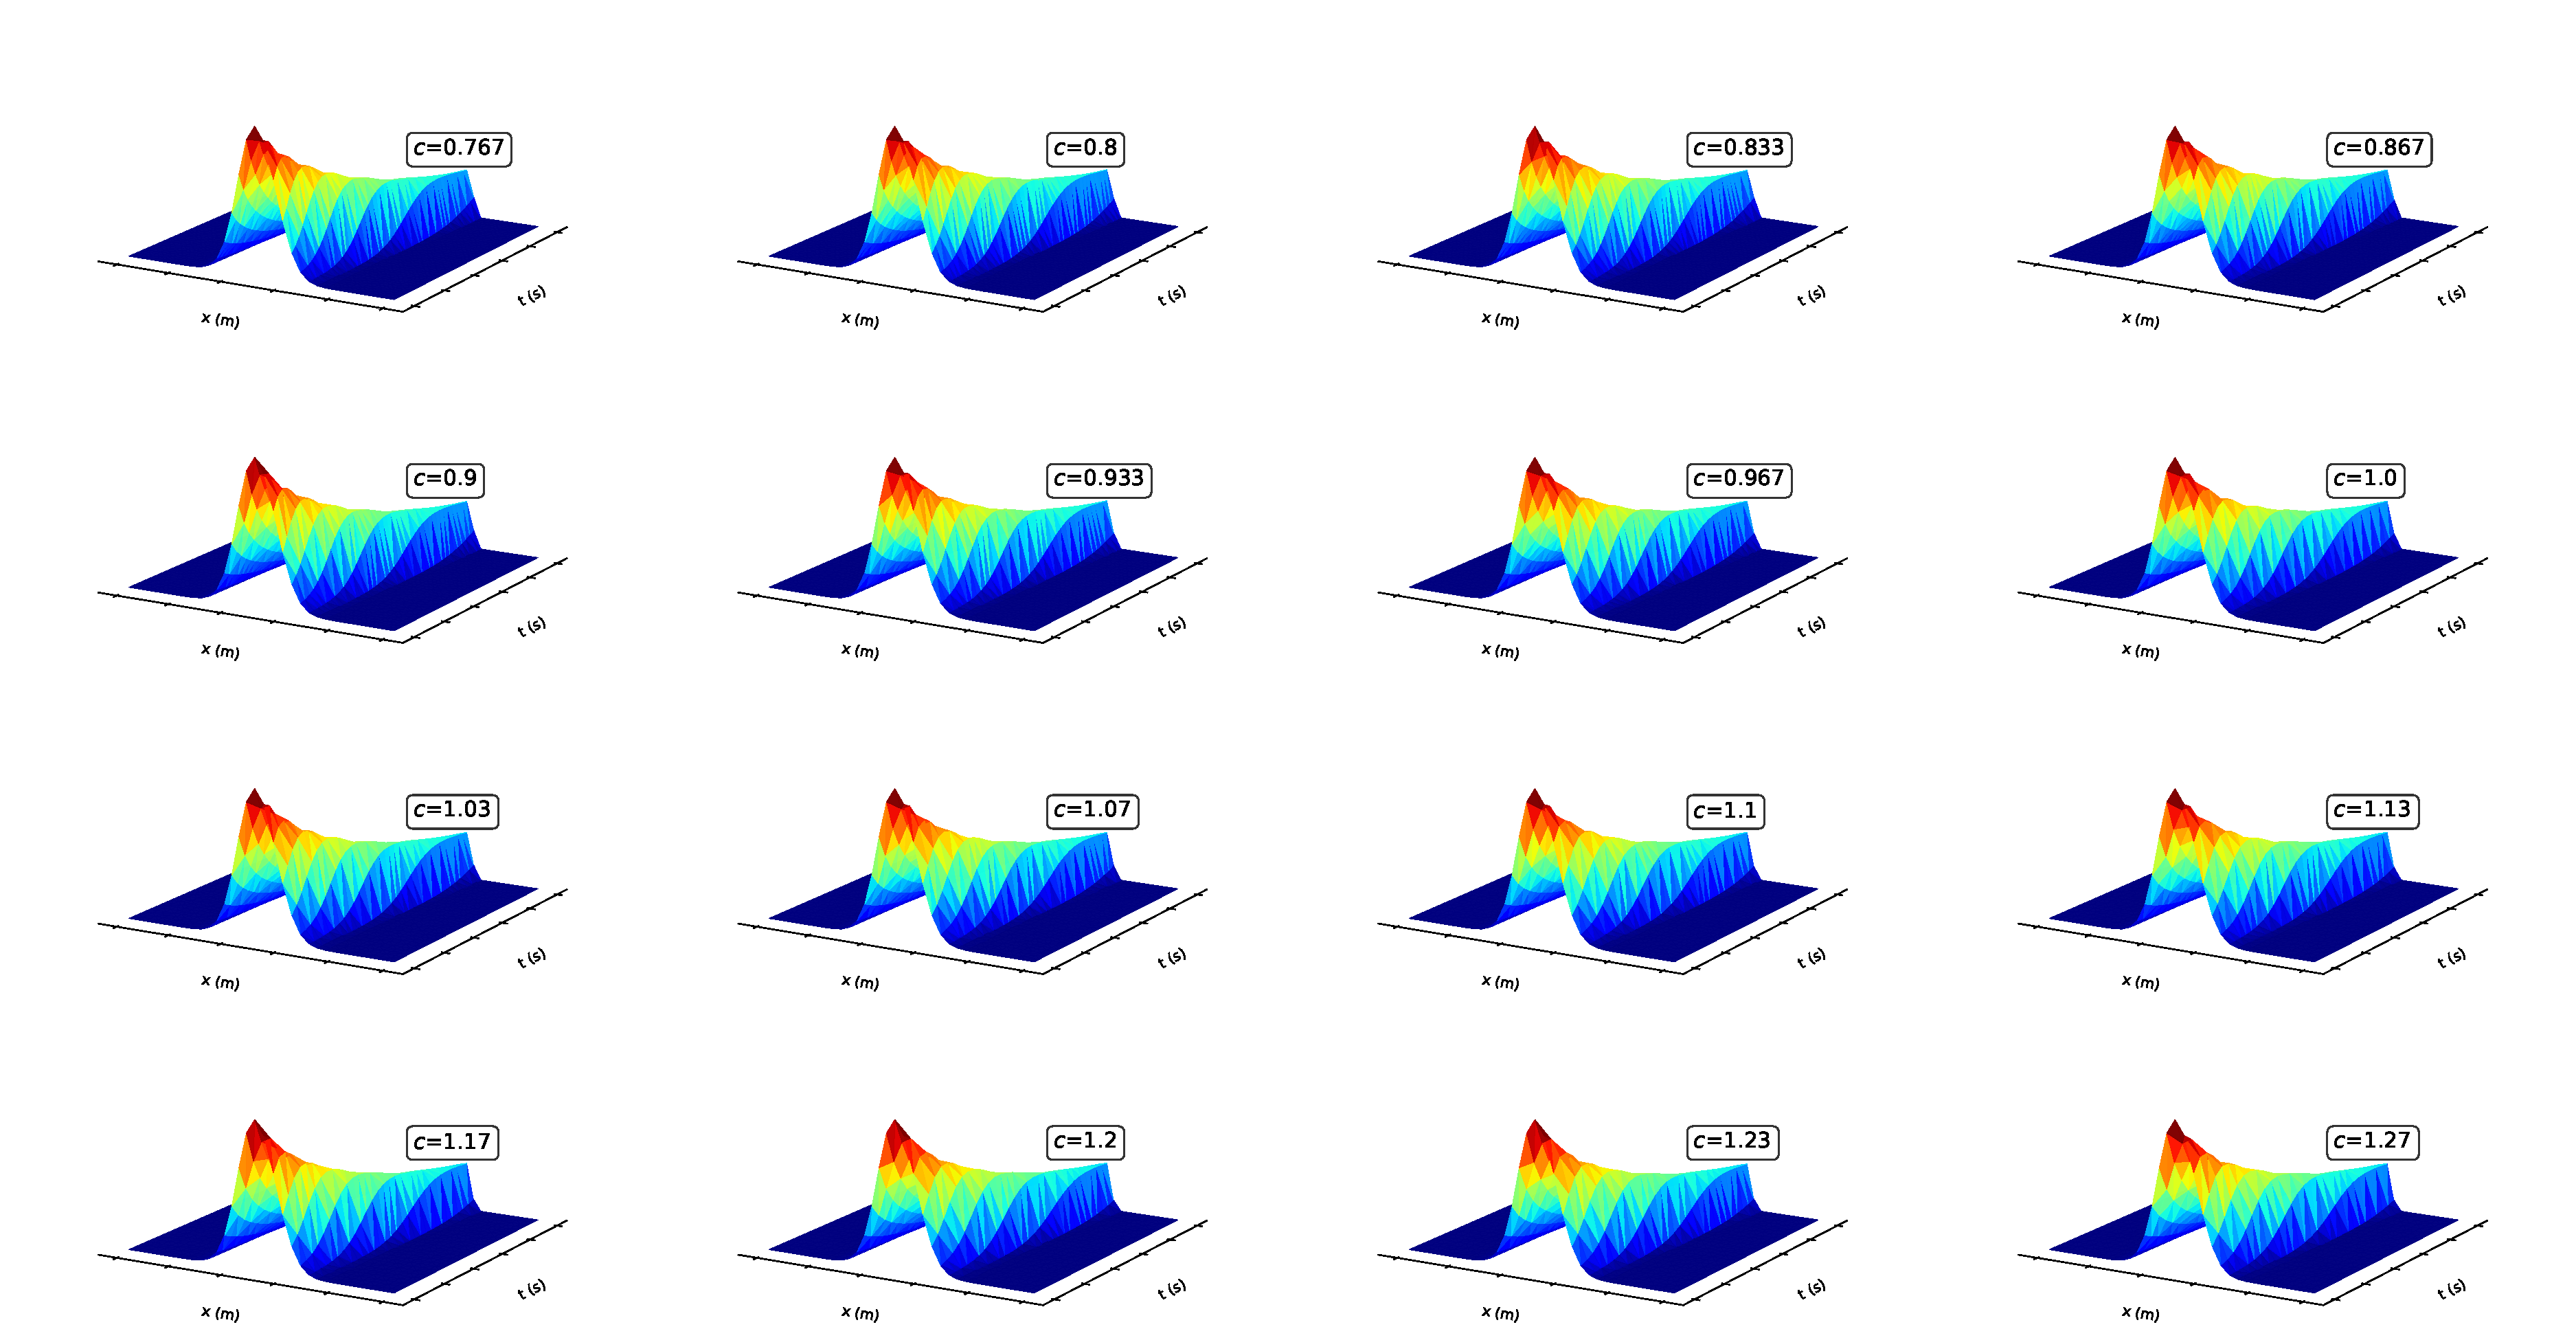
\includegraphics[width=\linewidth]{../BurgersEquation/images/multi_stable.pdf}\\
% \end{frame}

\begin{frame}
  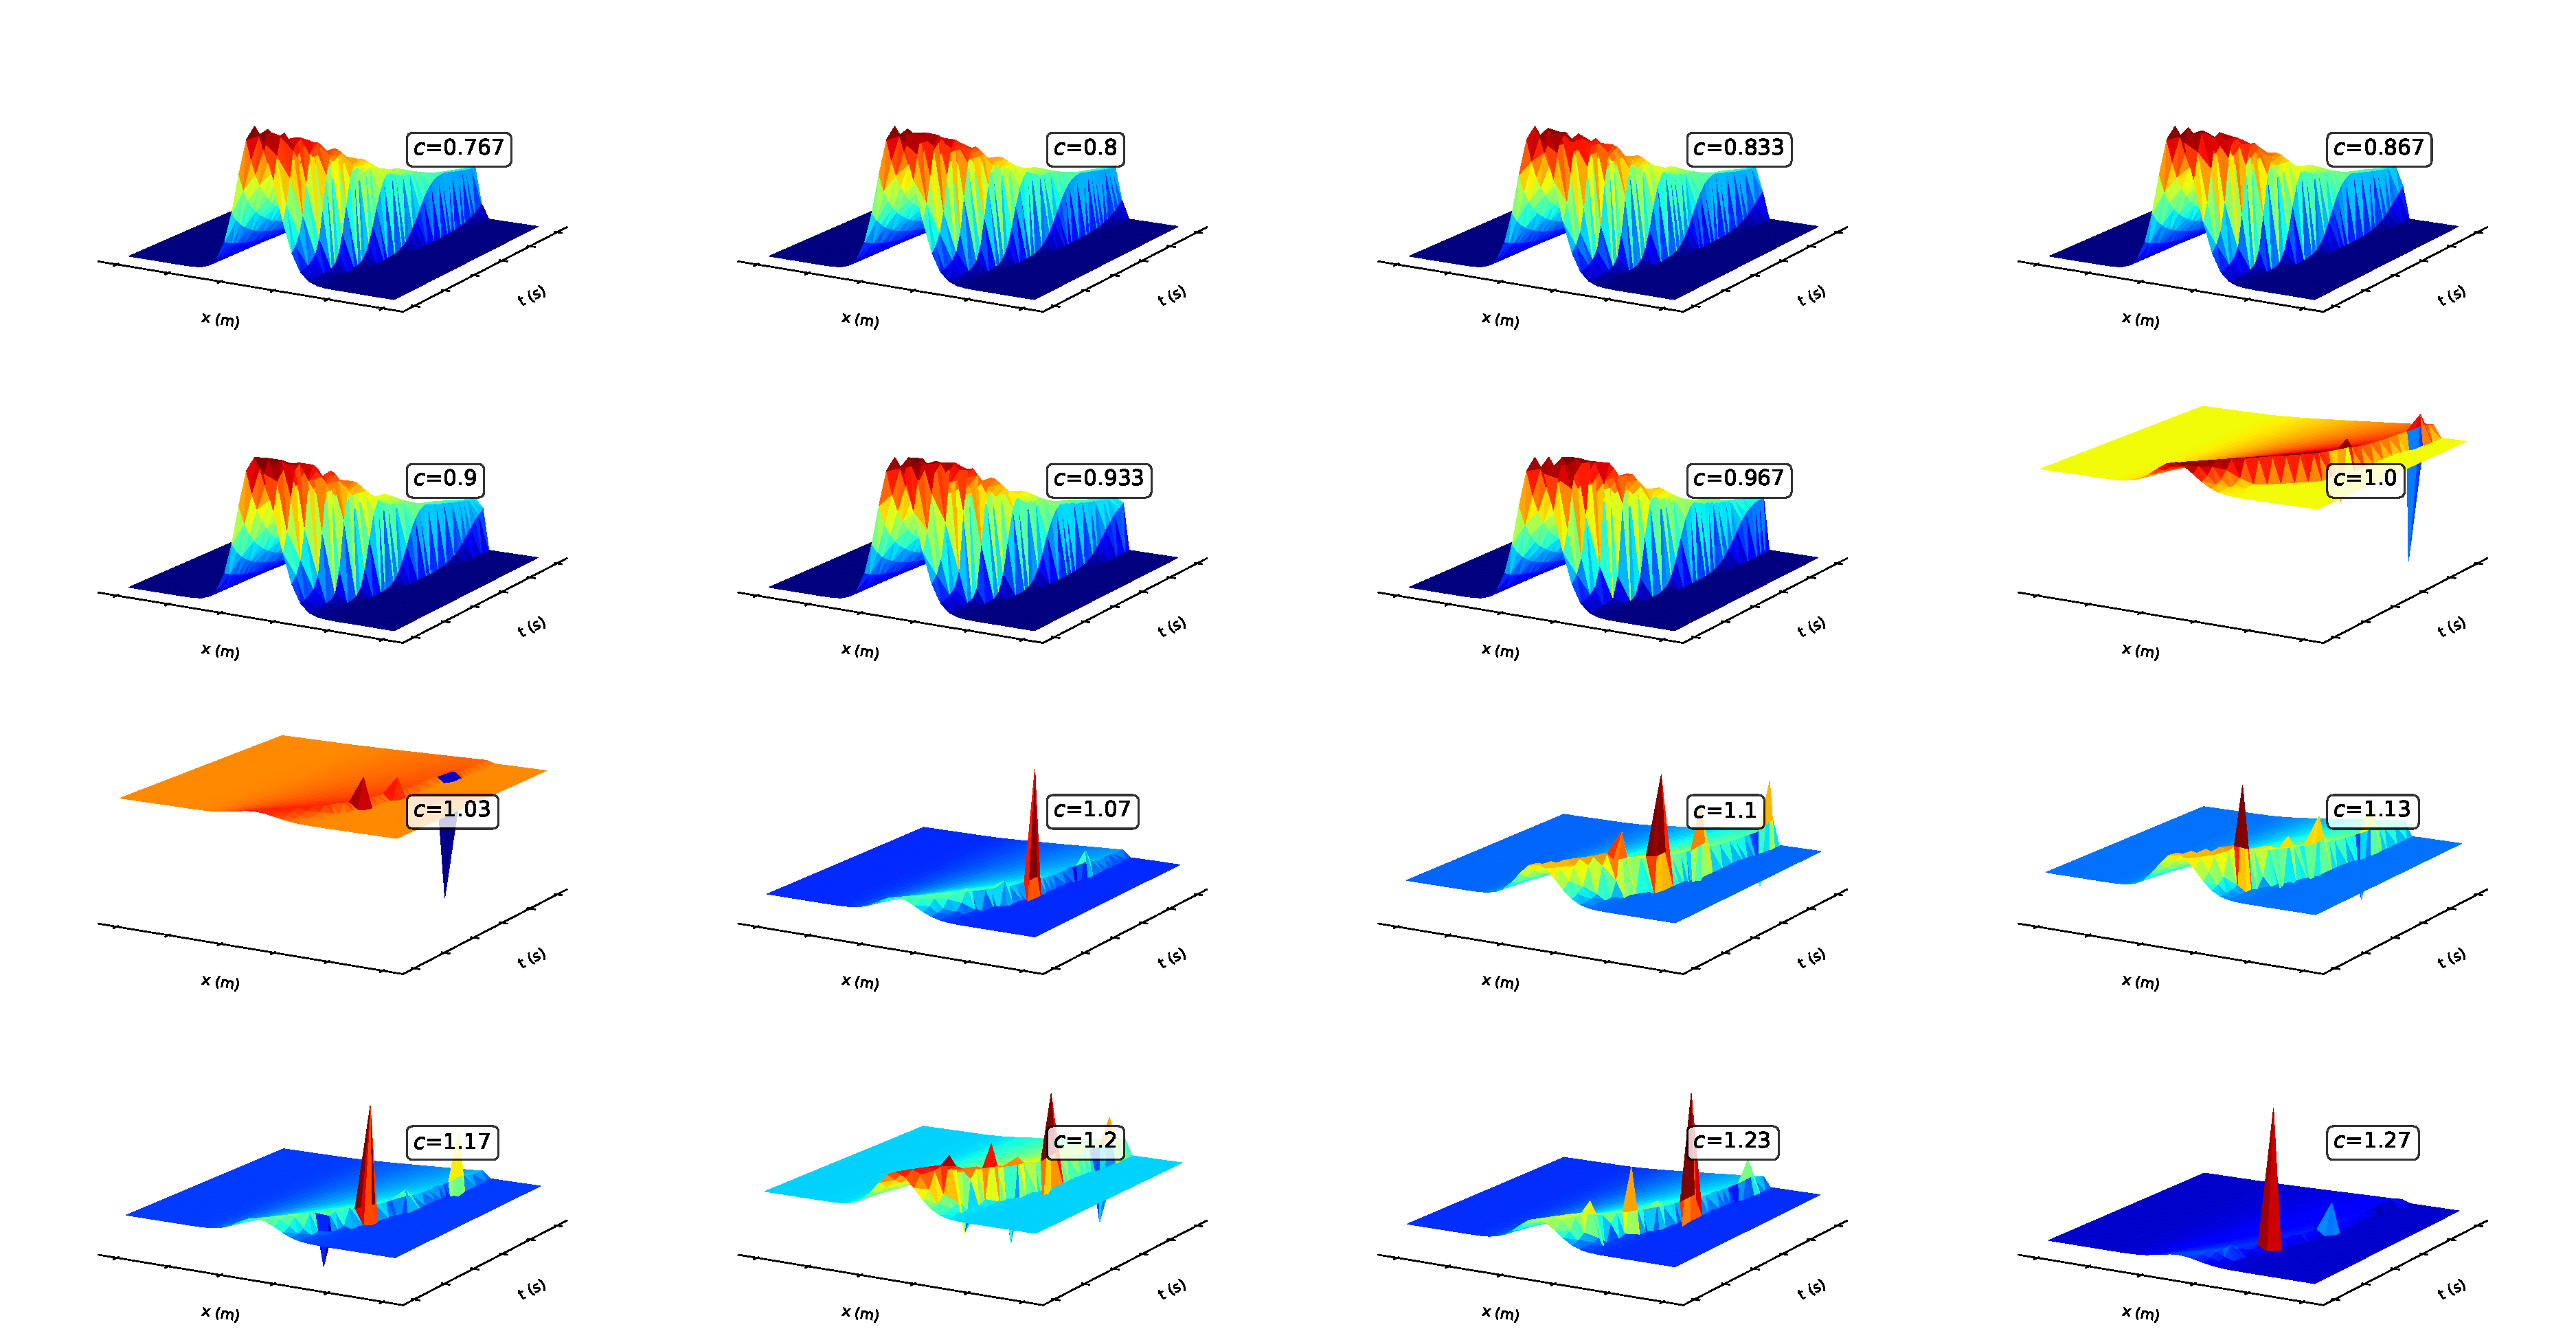
\includegraphics[width=\linewidth]{../BurgersEquation/images/multi_unstable.pdf}\\
\end{frame}


% 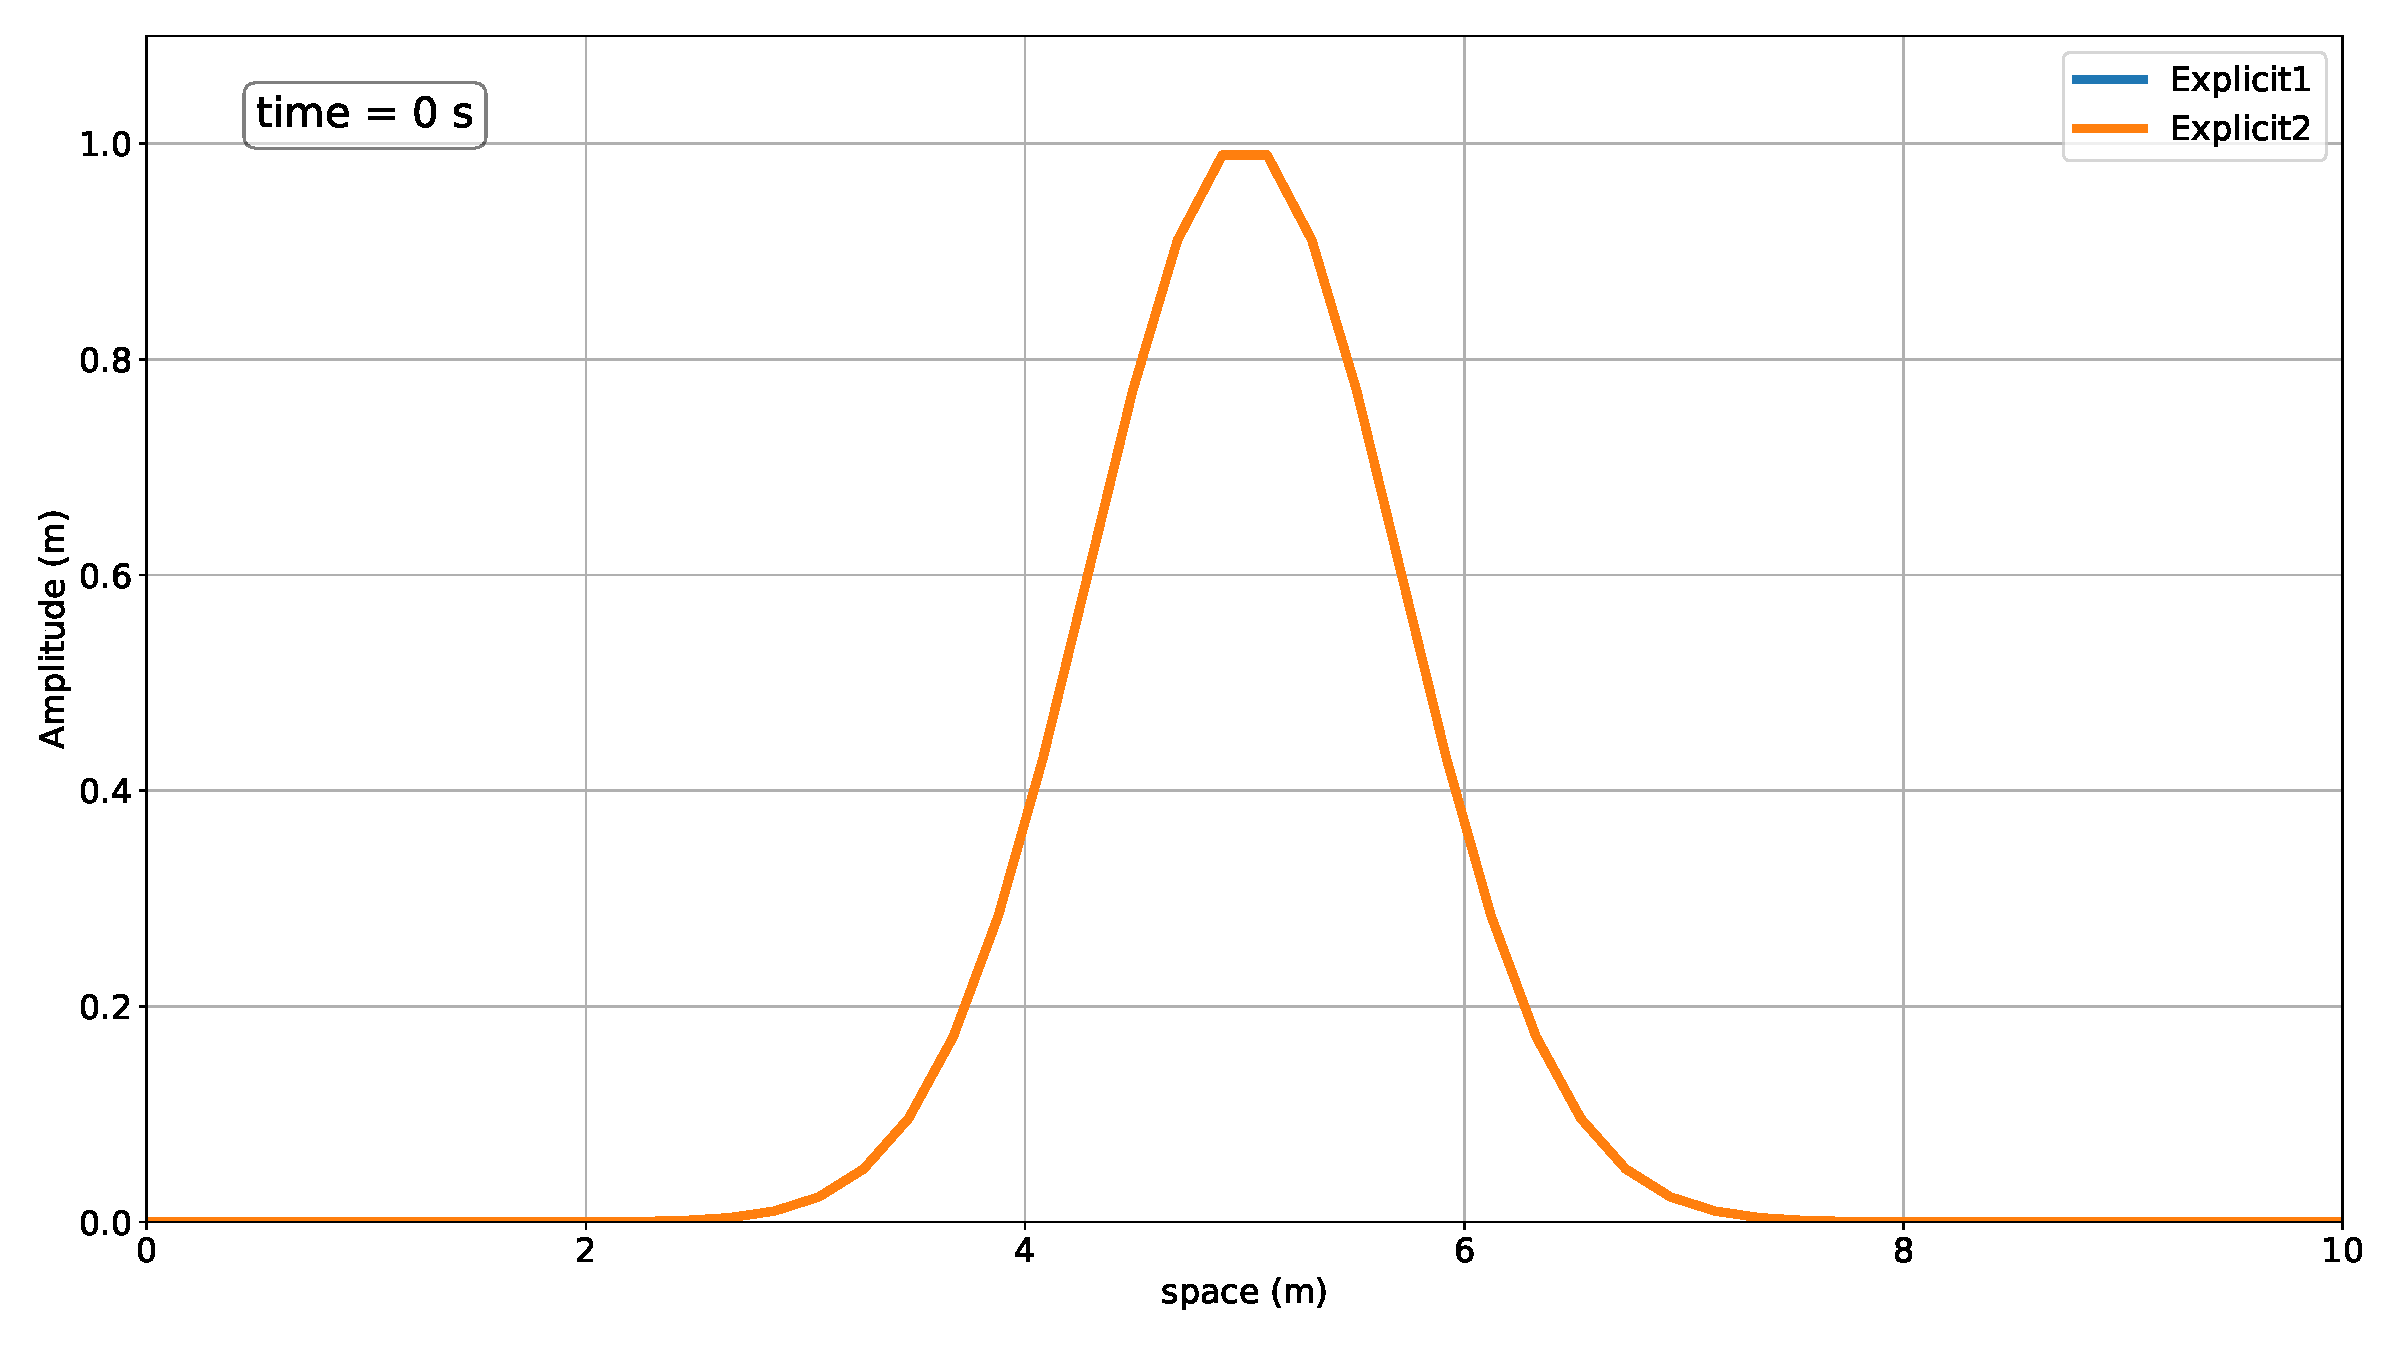
\includegraphics[width=\linewidth]{../BurgersEquation/images/expl0.pdf}
% 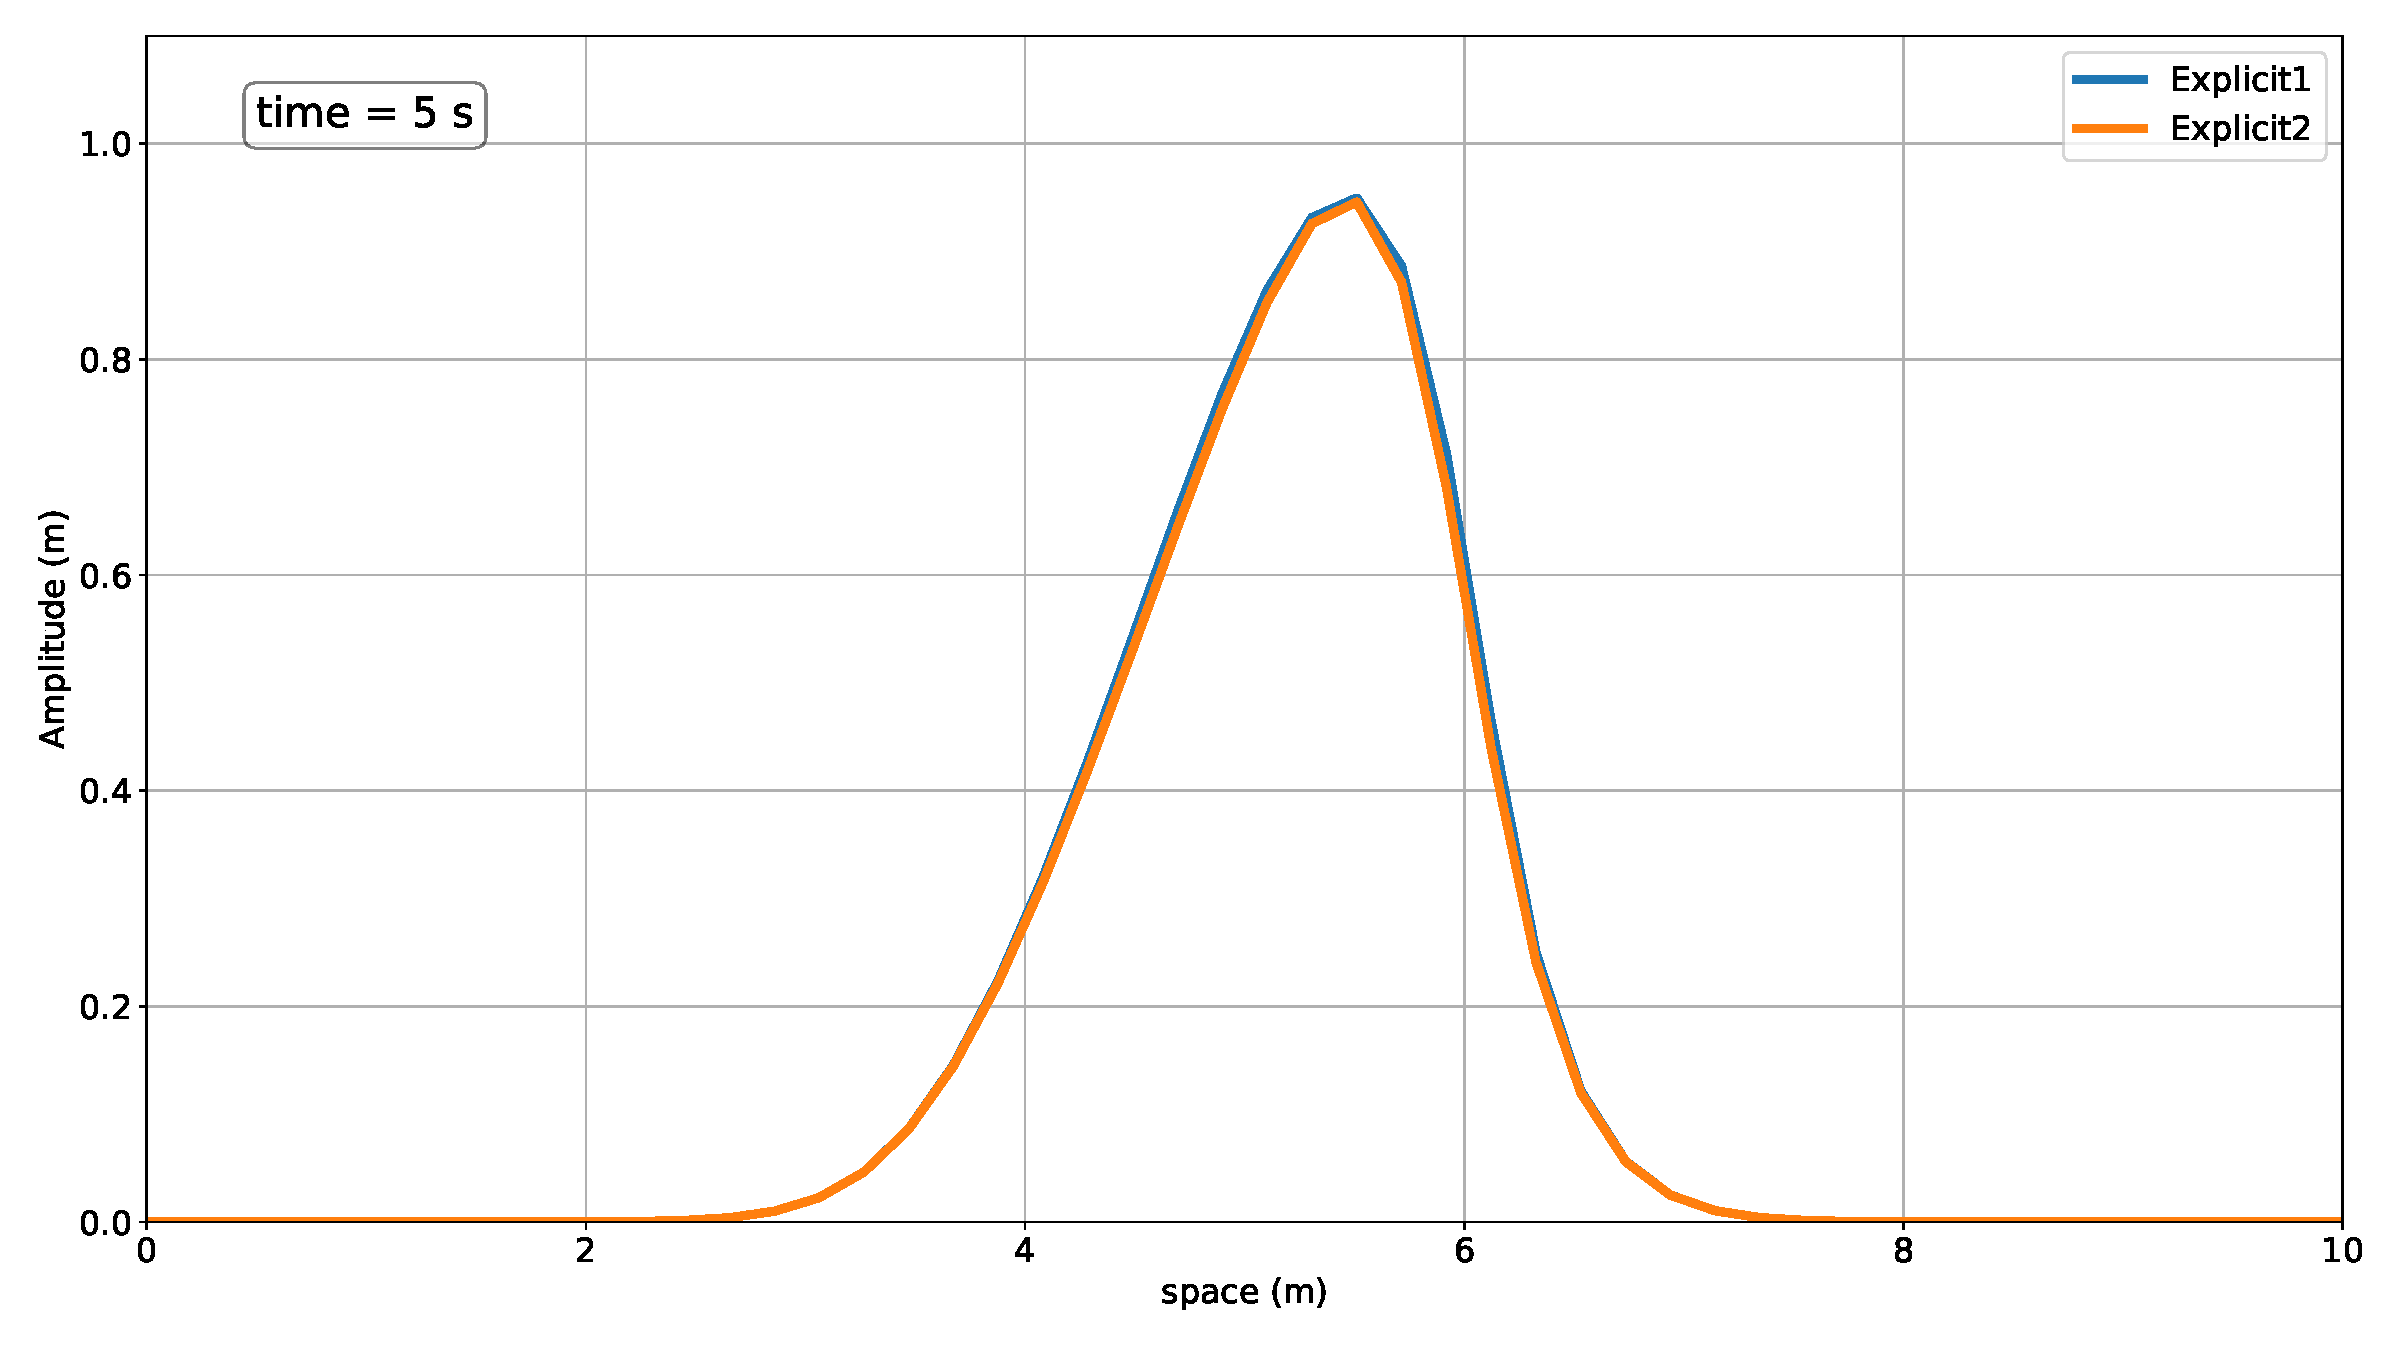
\includegraphics[width=\linewidth]{../BurgersEquation/images/expl1.pdf}
% 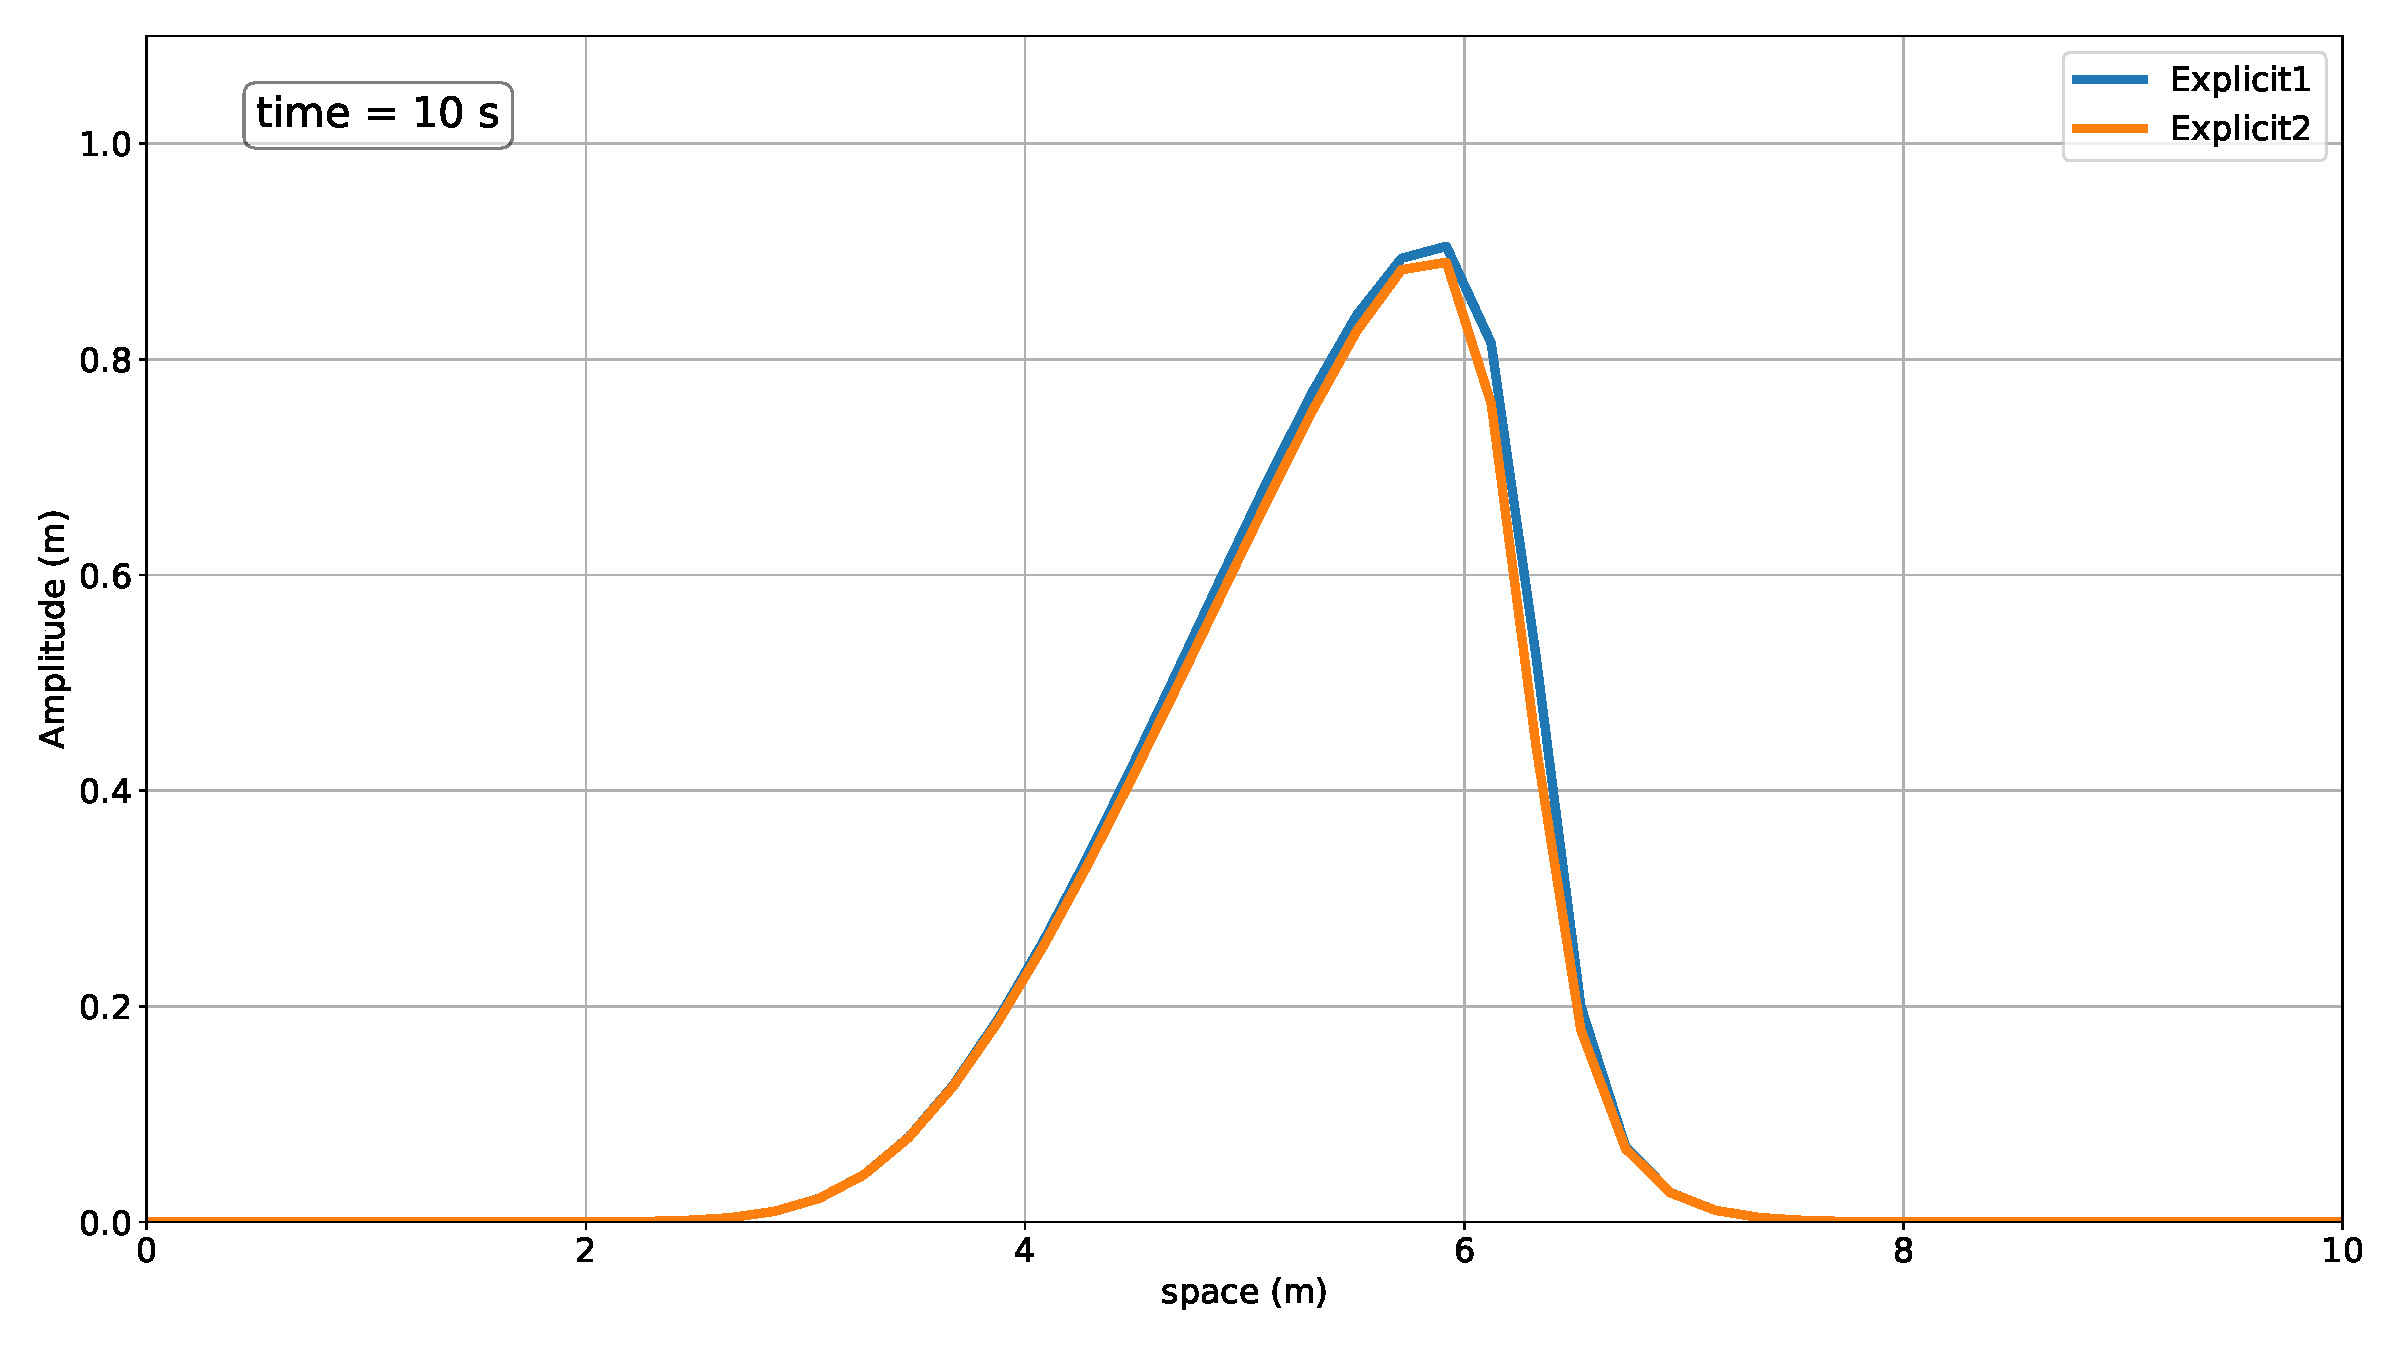
\includegraphics[width=\linewidth]{../BurgersEquation/images/expl2.pdf}
% 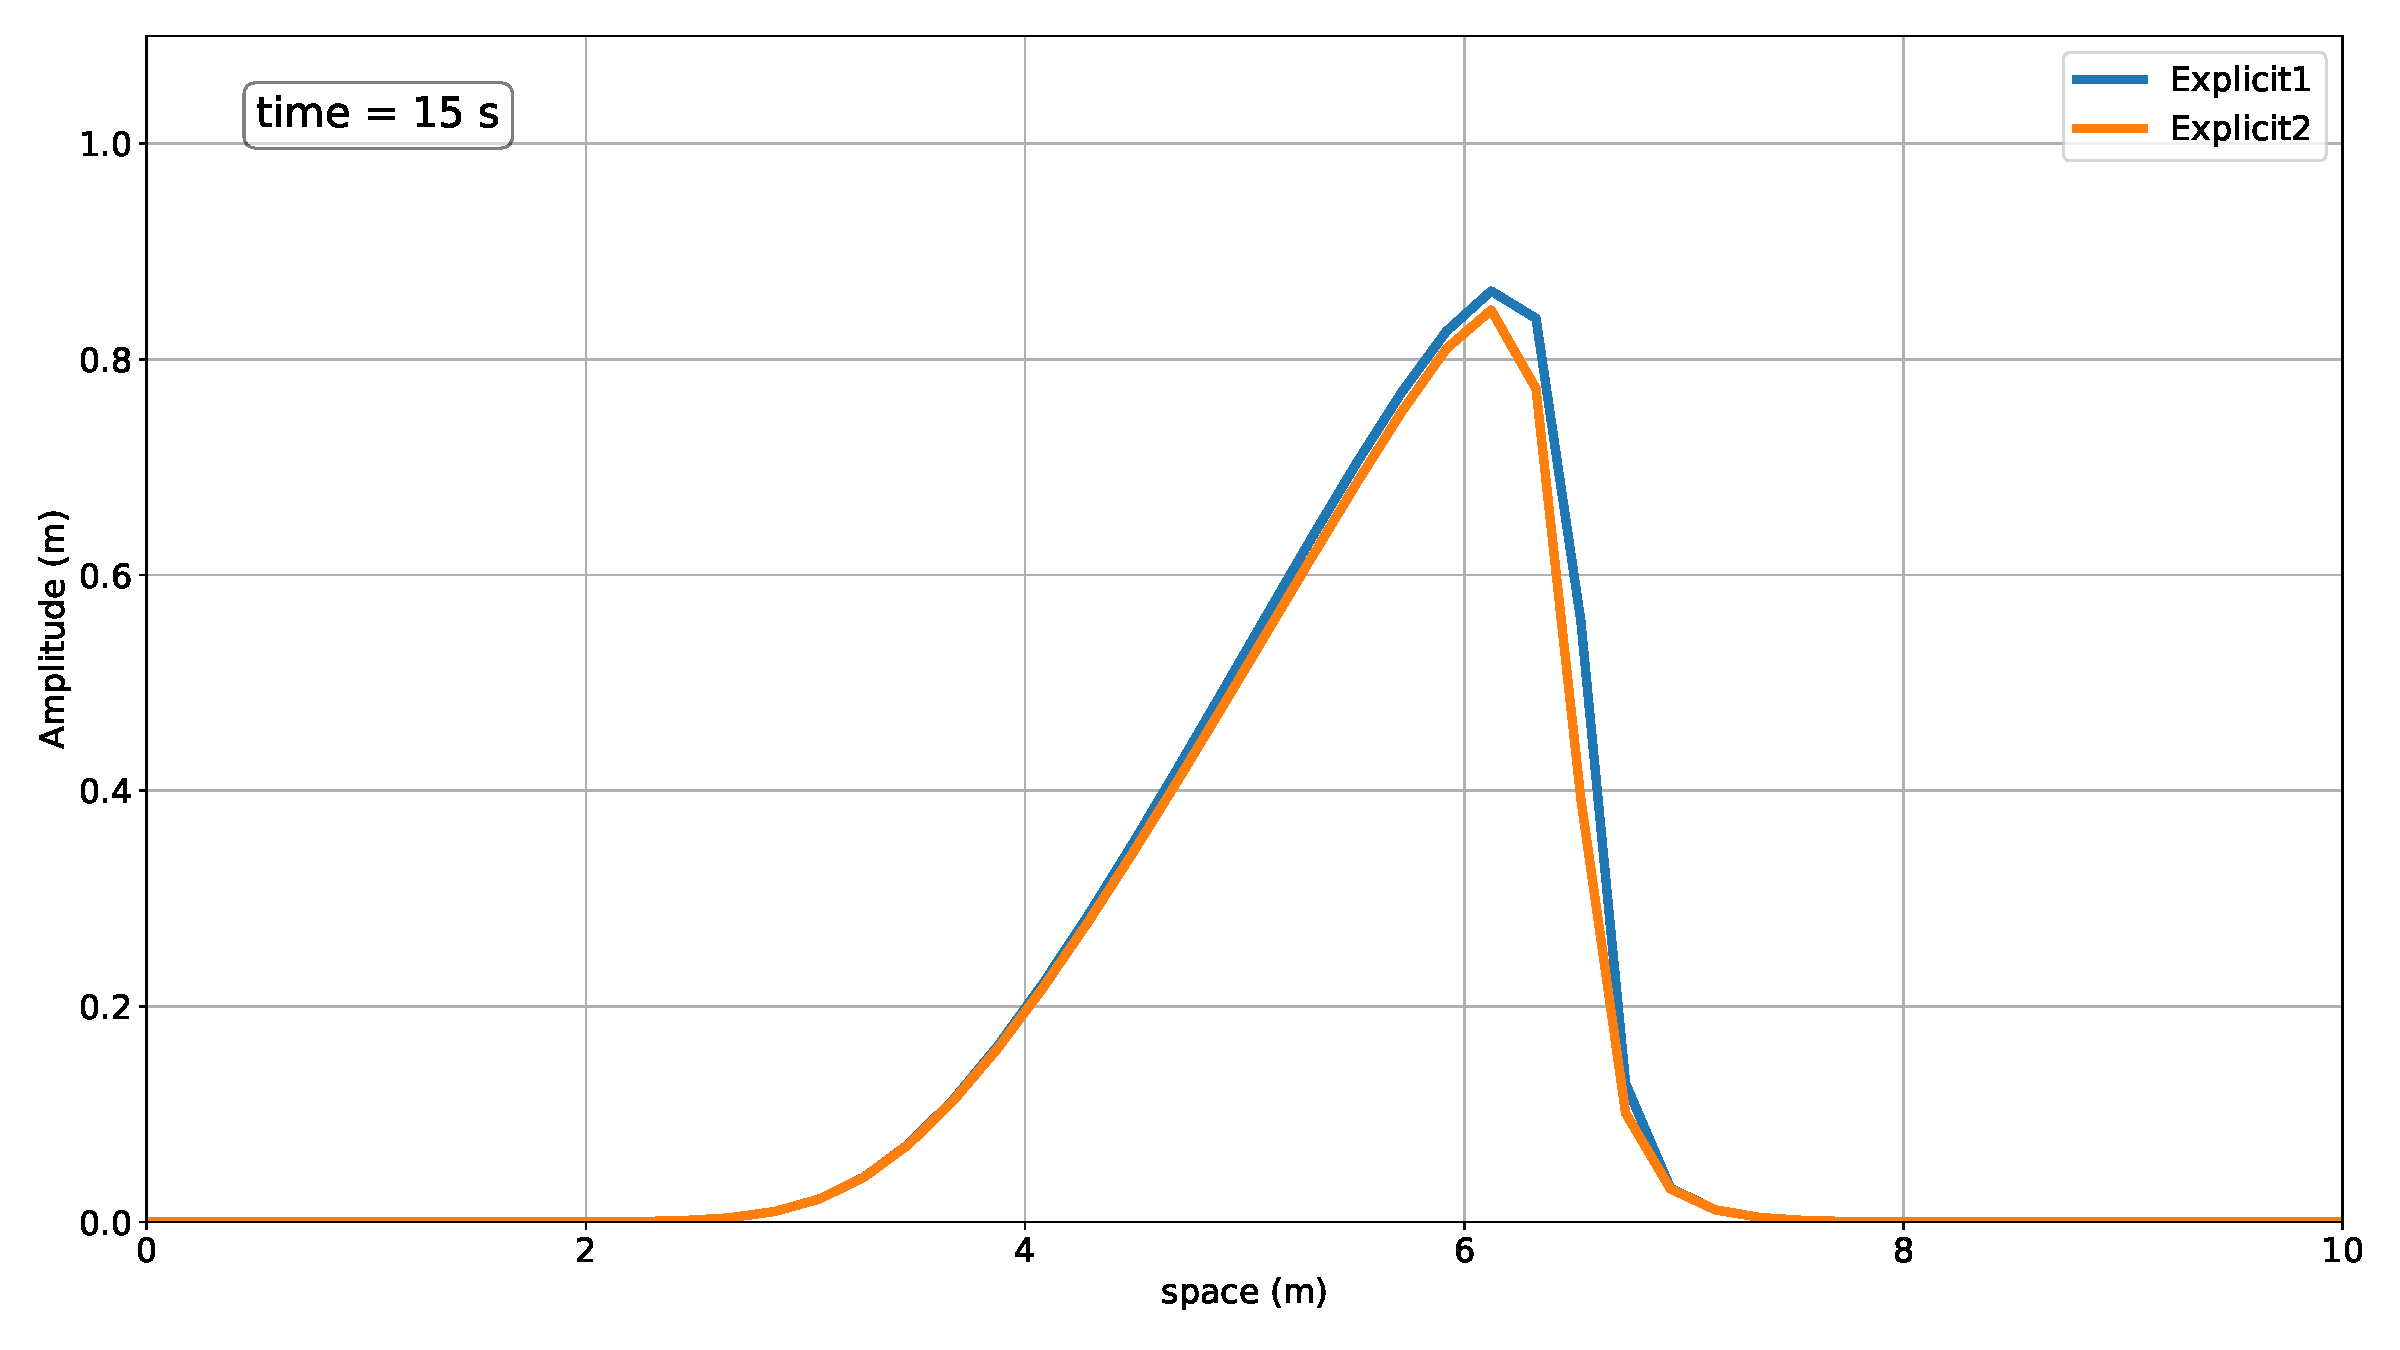
\includegraphics[width=\linewidth]{../BurgersEquation/images/expl3.pdf}
% 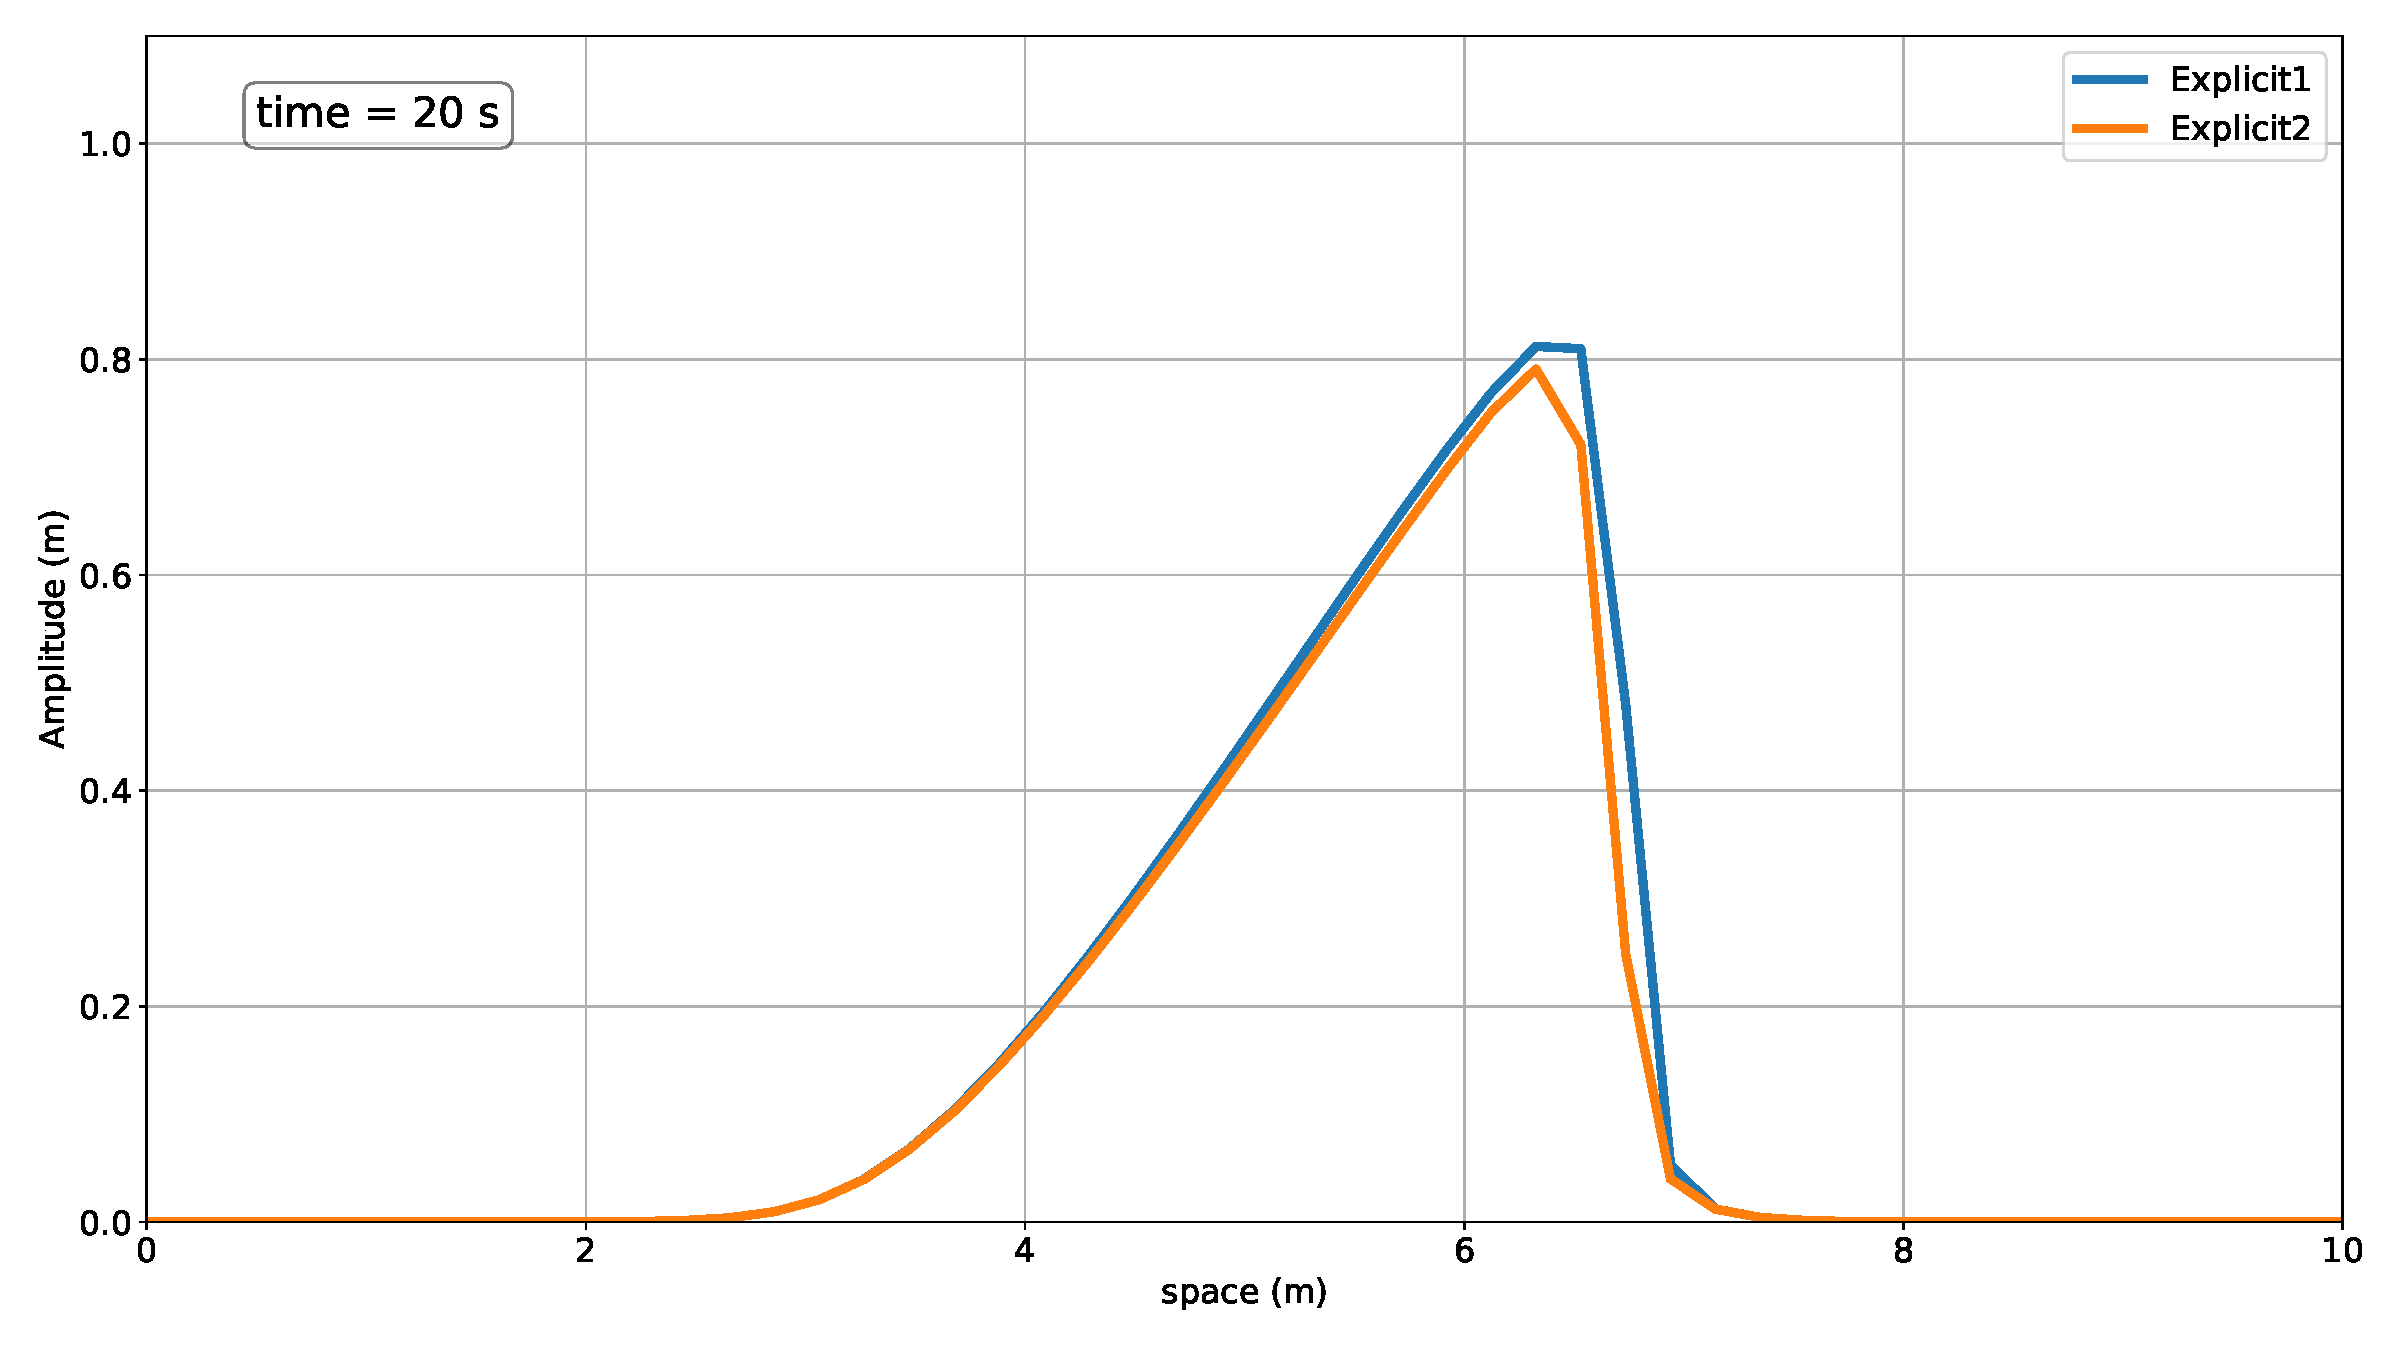
\includegraphics[width=\linewidth]{../BurgersEquation/images/expl4.pdf}
% 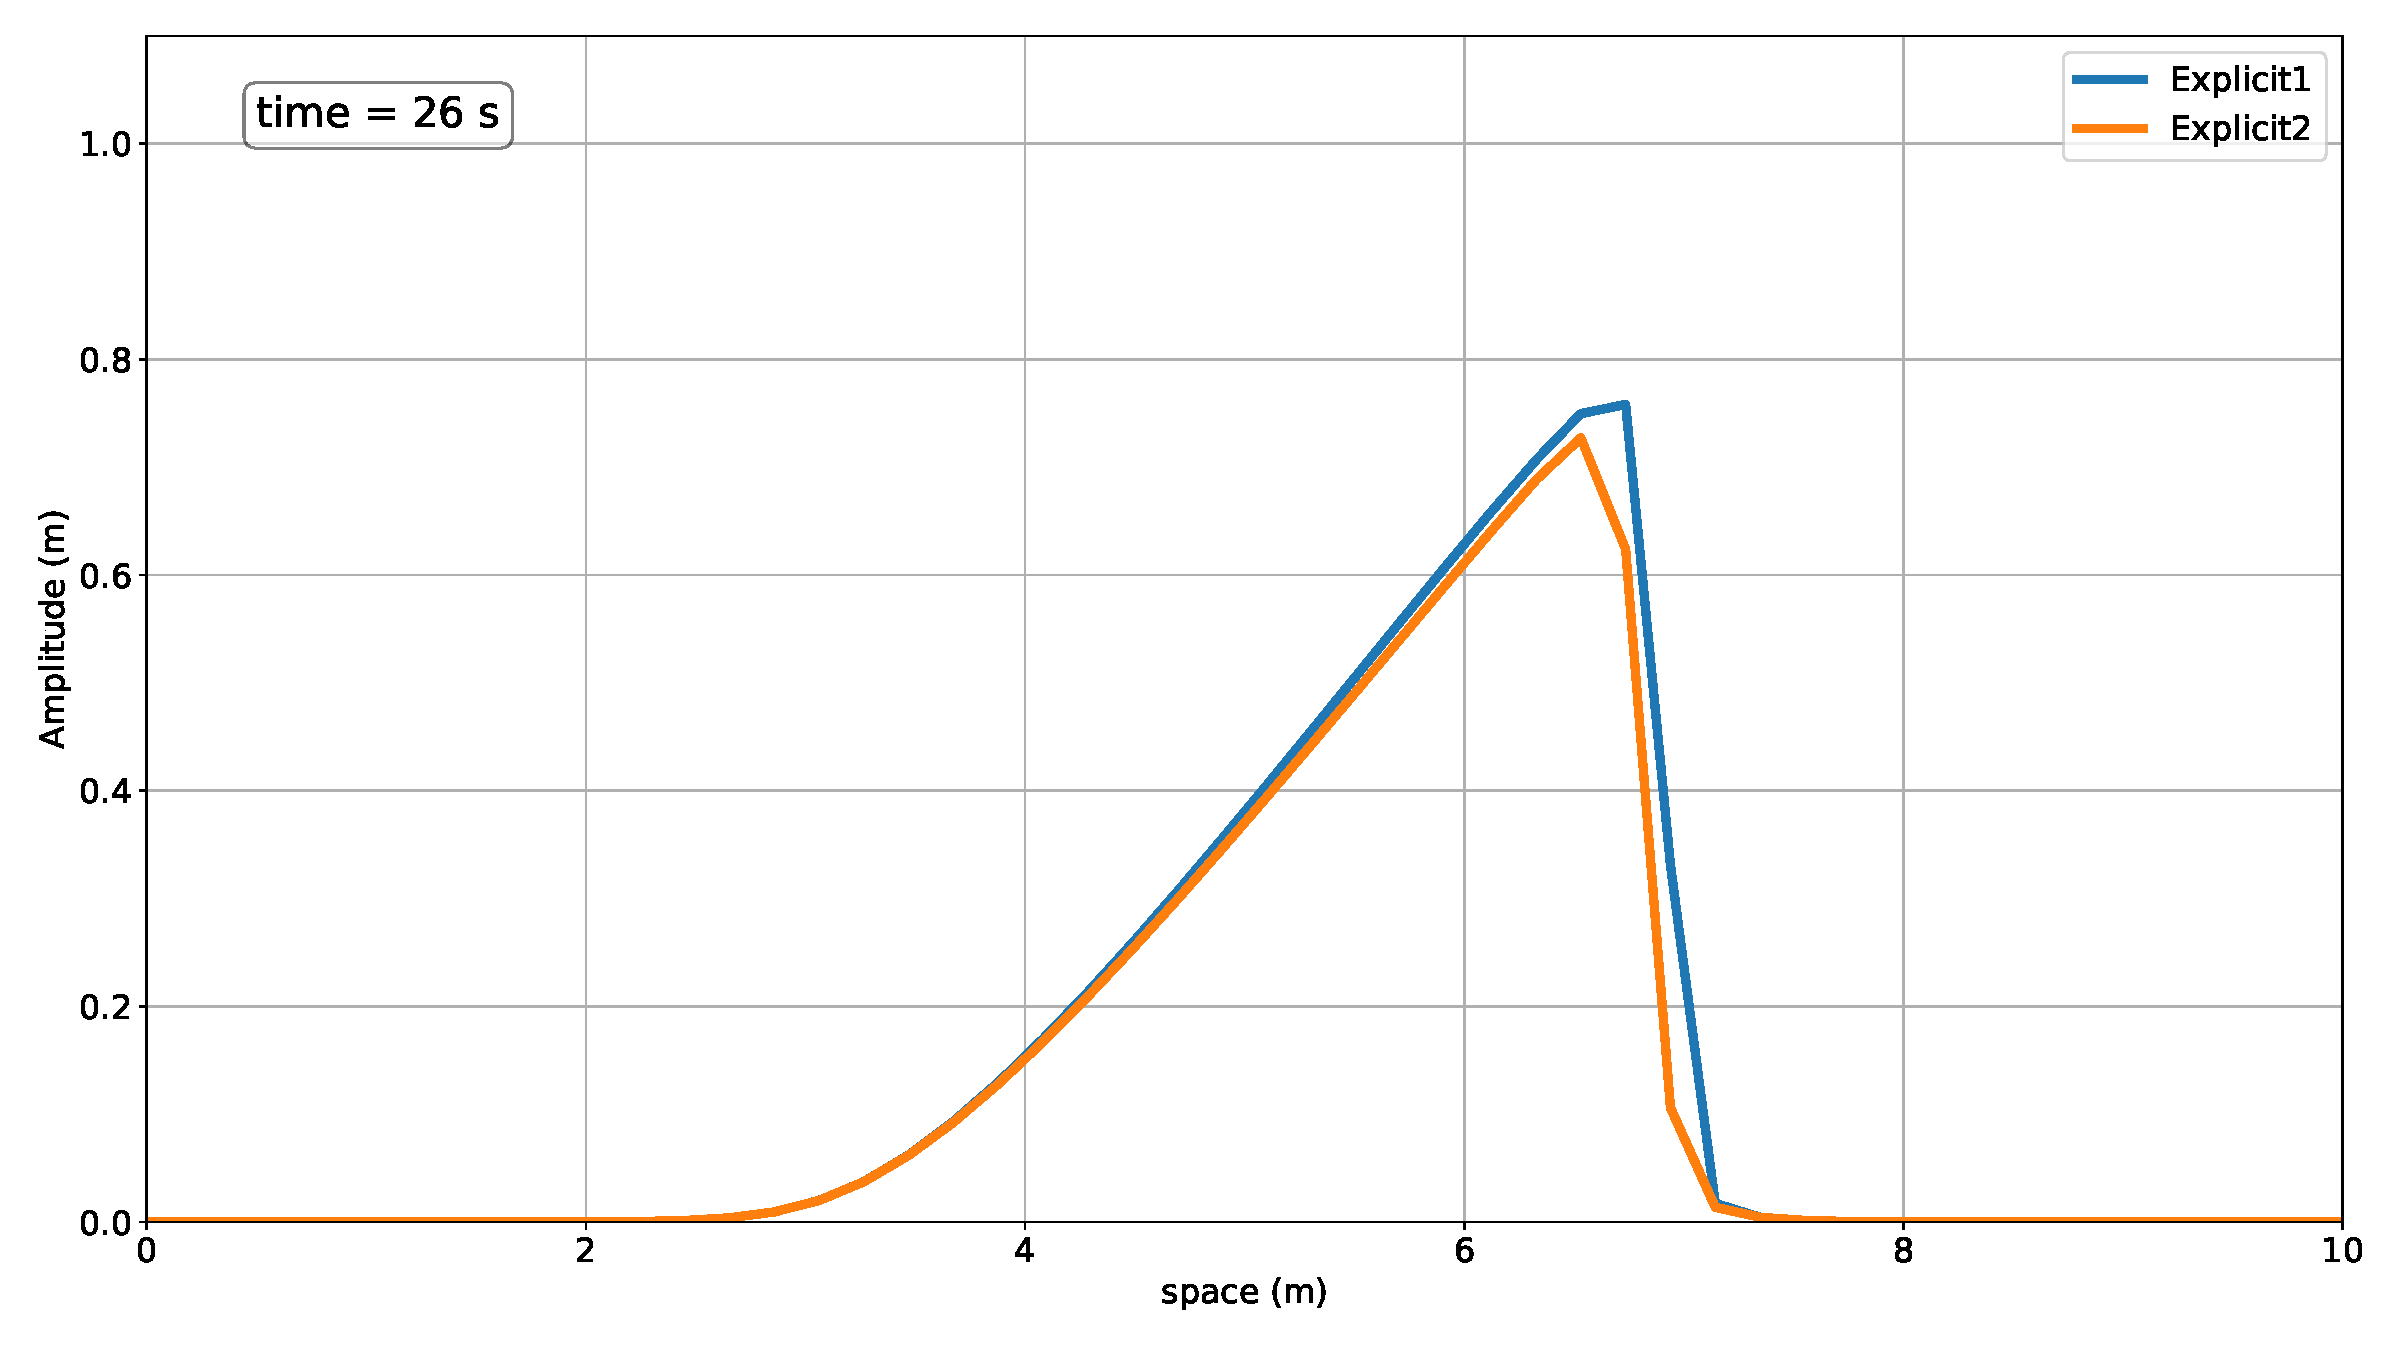
\includegraphics[width=\linewidth]{../BurgersEquation/images/expl5.pdf}
% 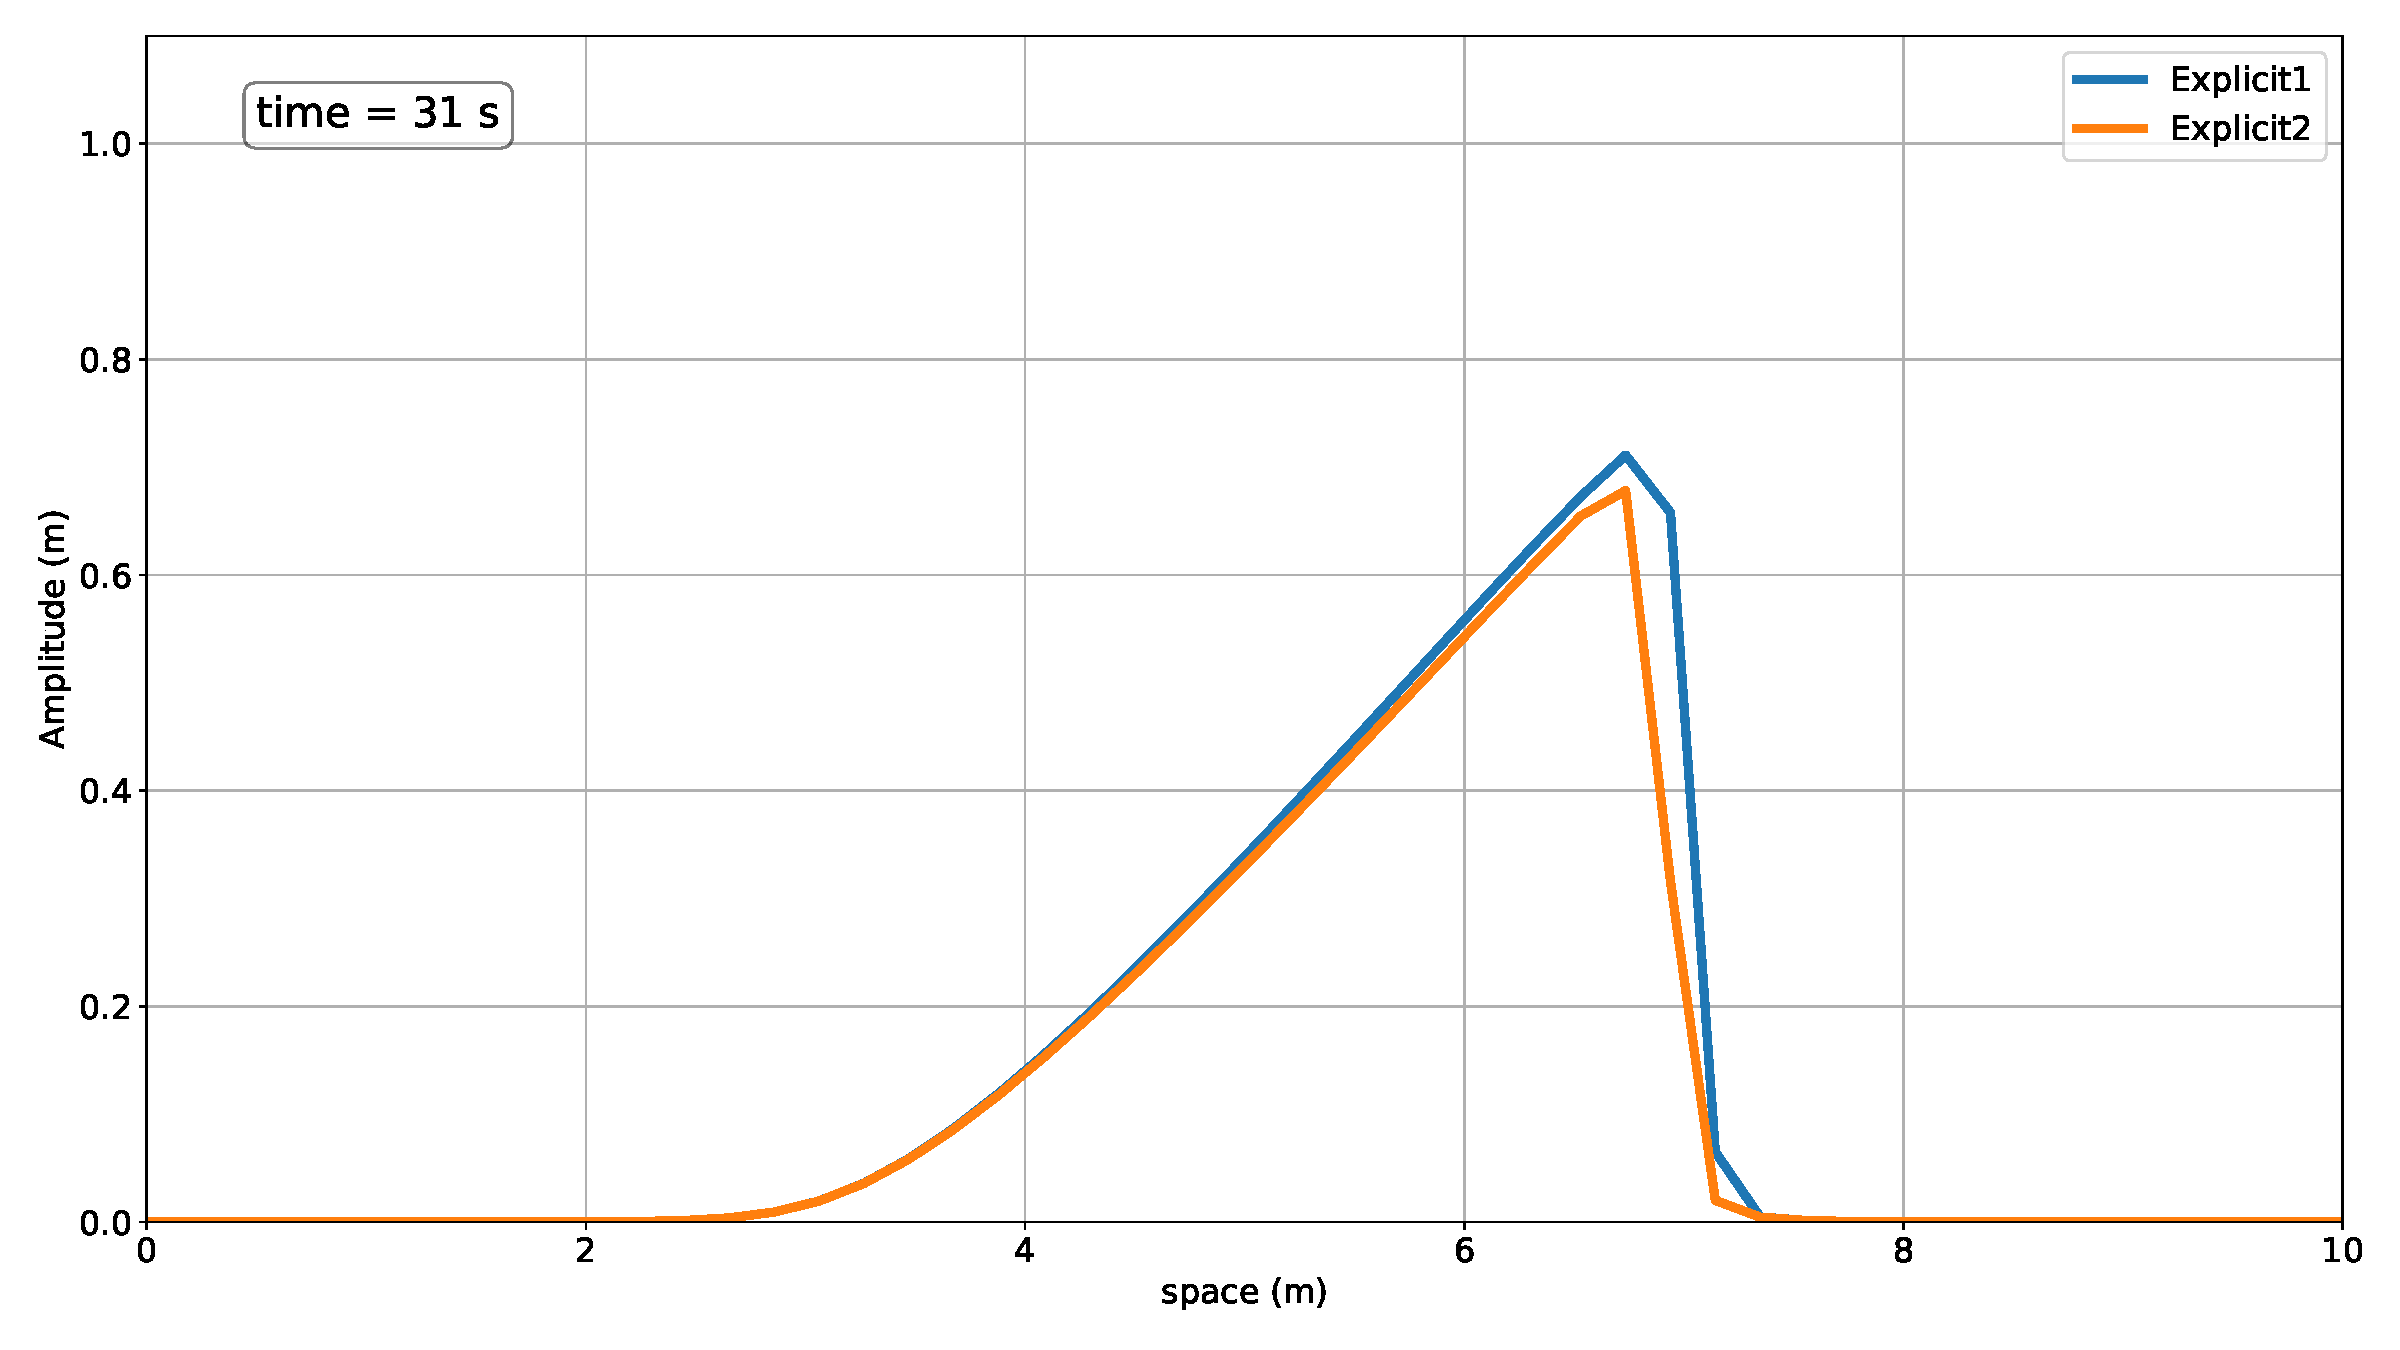
\includegraphics[width=\linewidth]{../BurgersEquation/images/expl6.pdf}
% 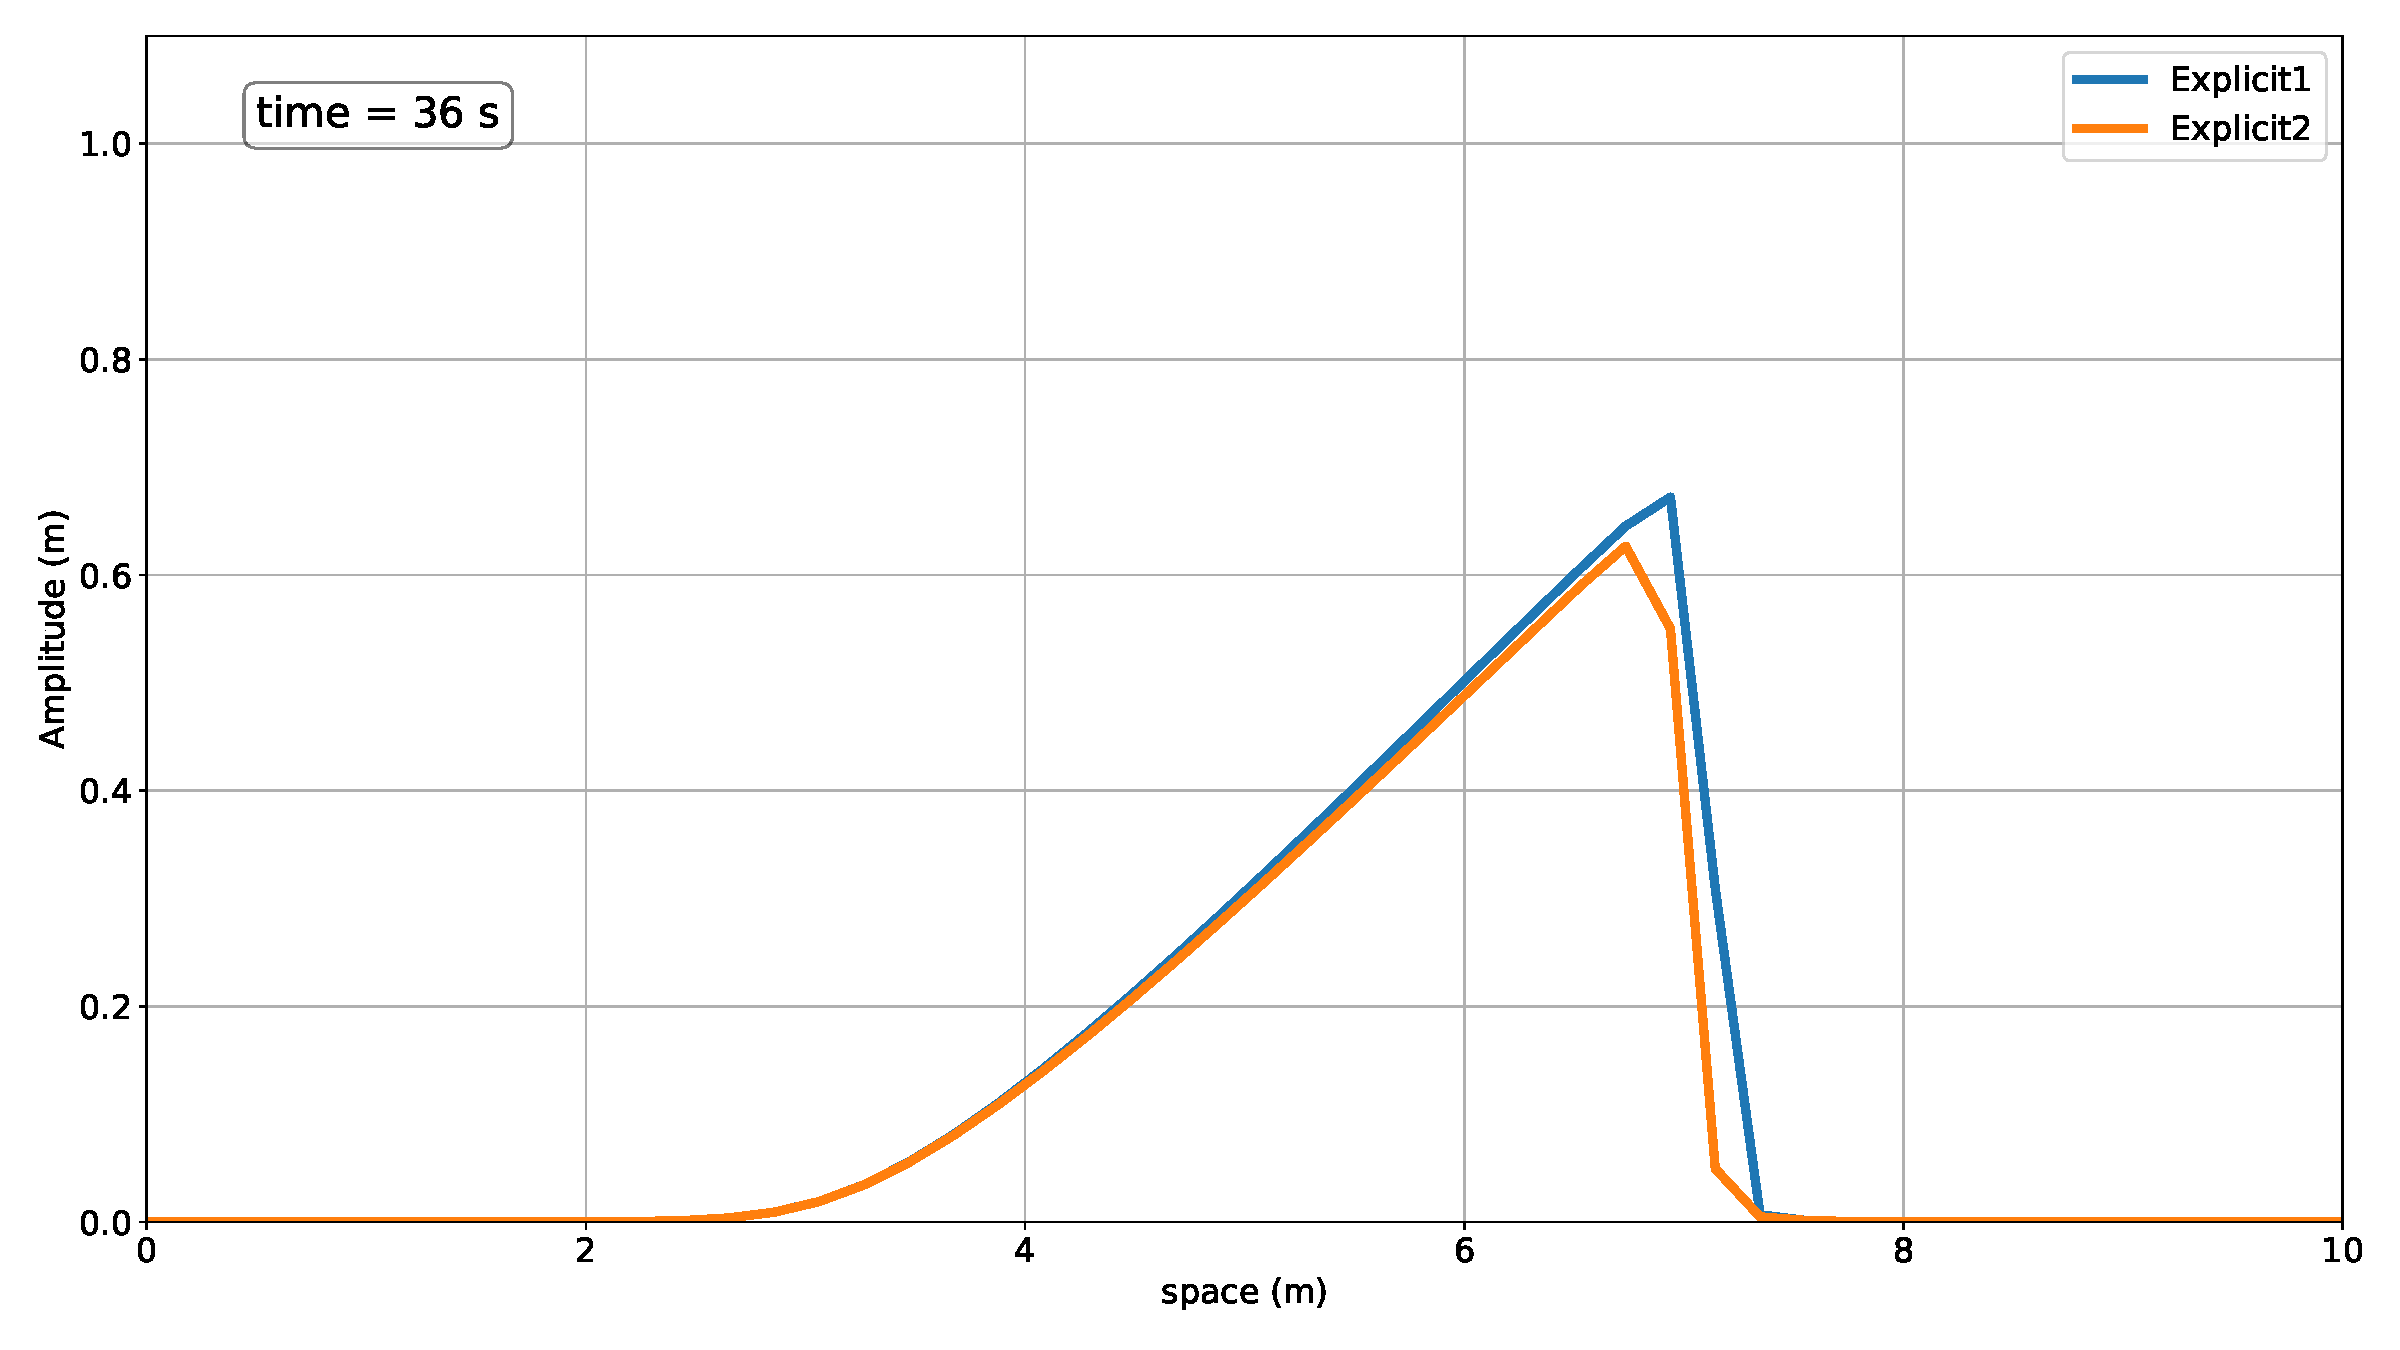
\includegraphics[width=\linewidth]{../BurgersEquation/images/expl7.pdf}
% 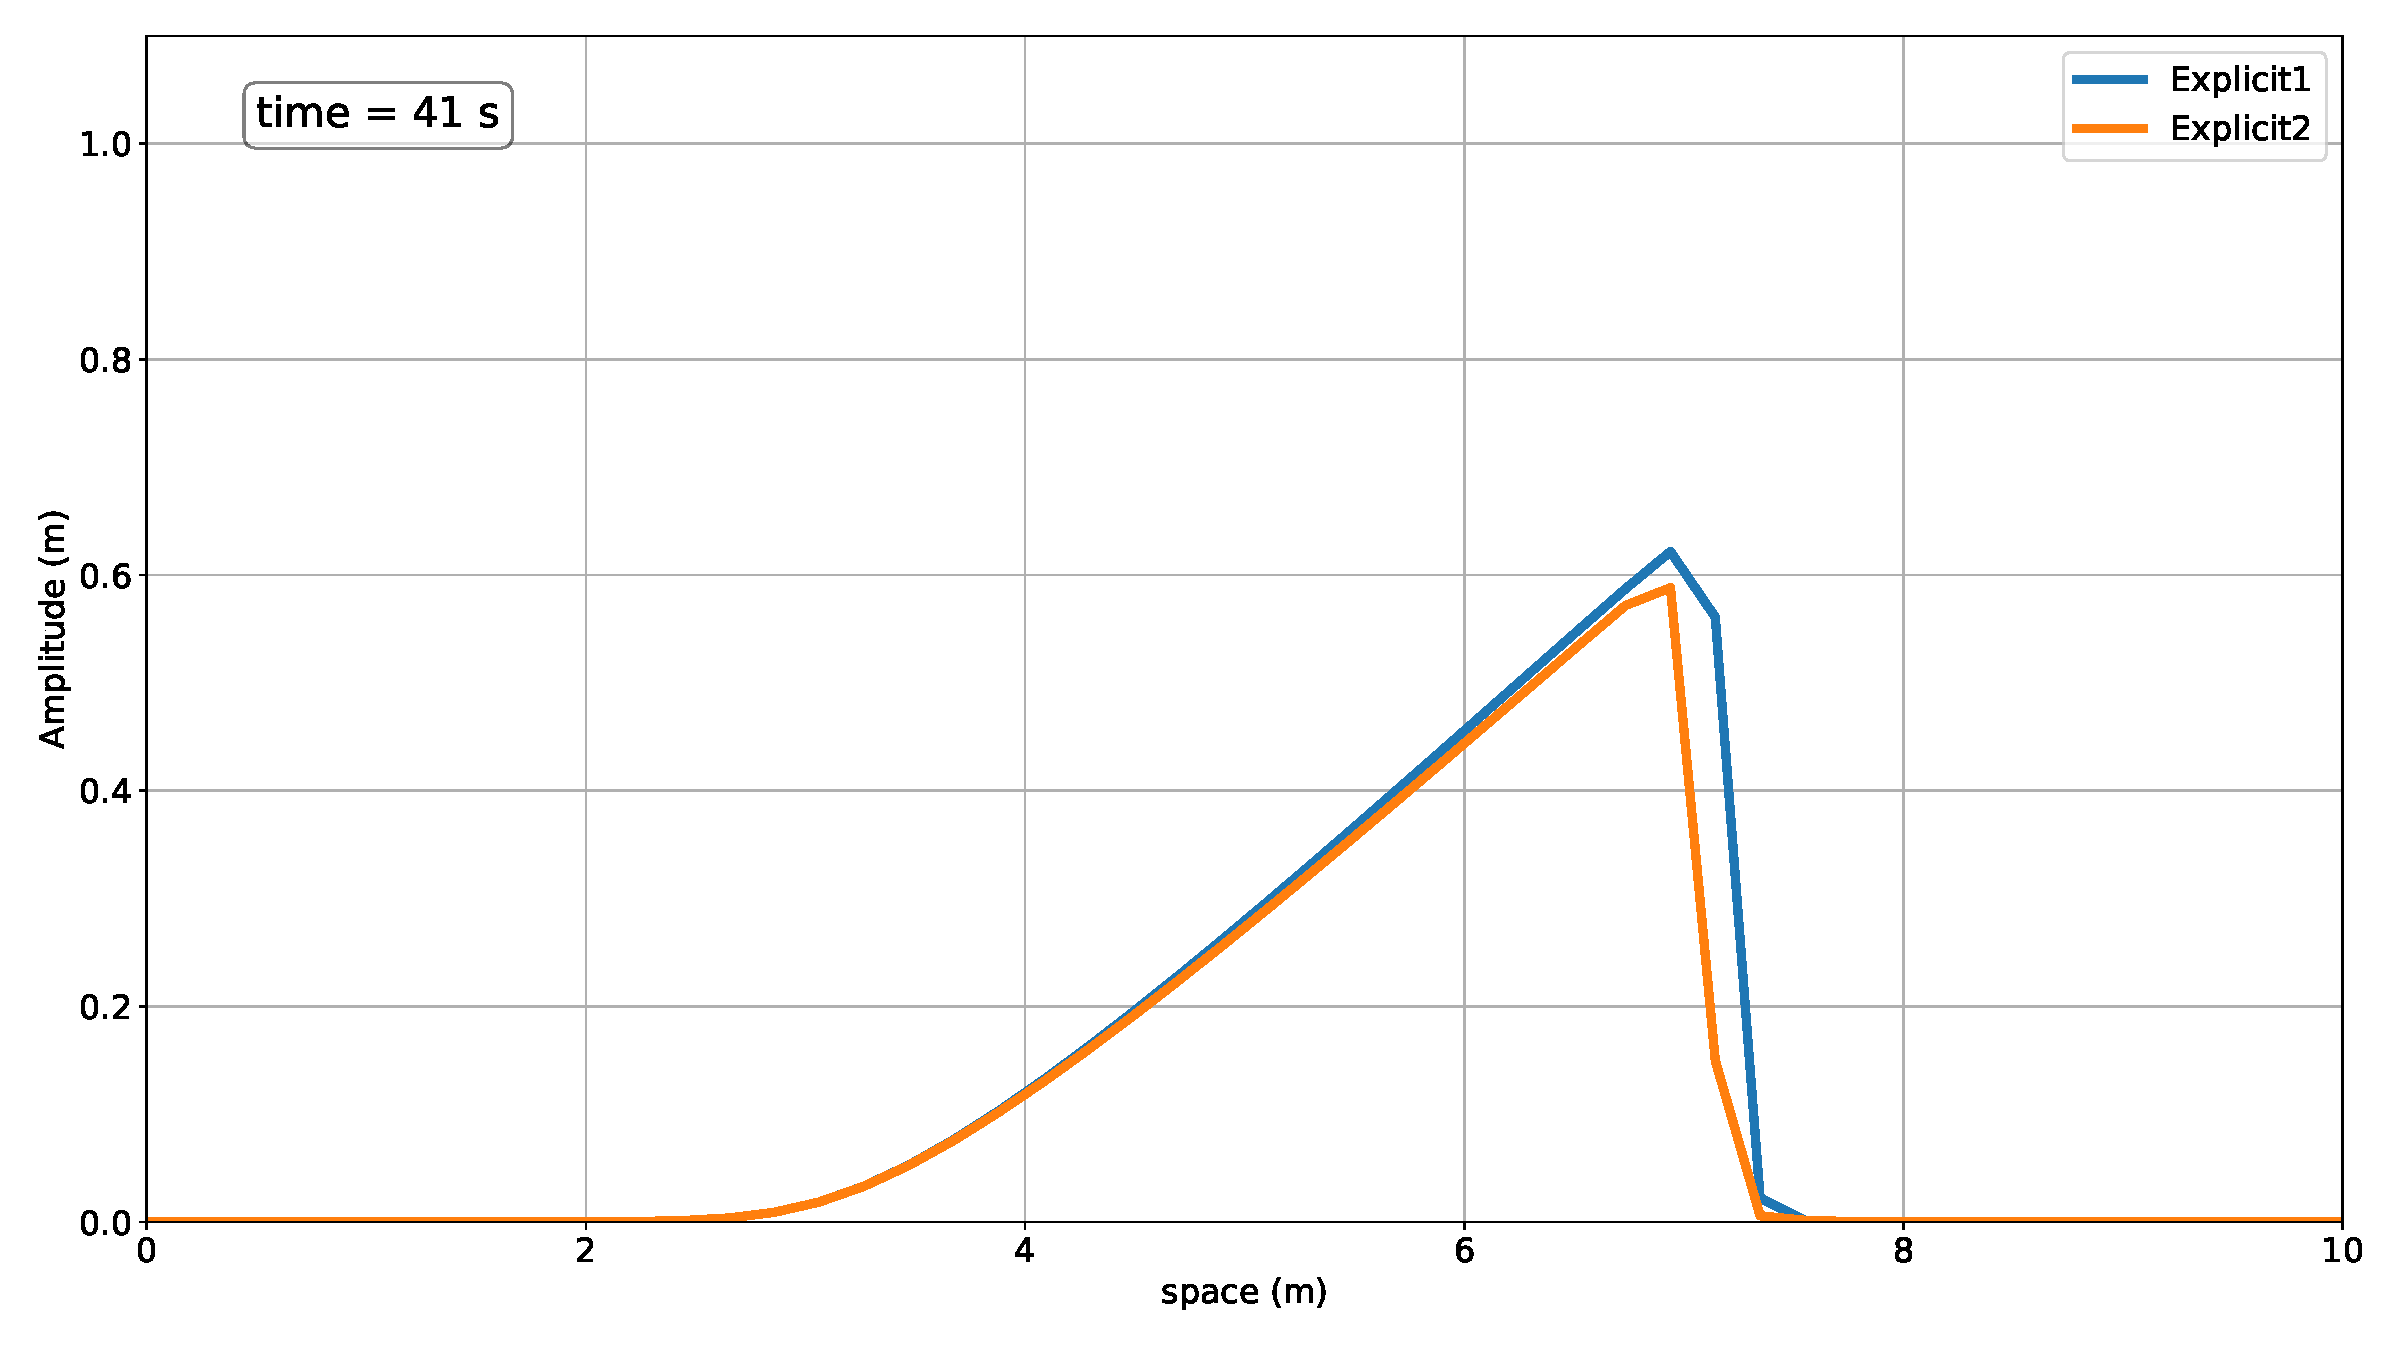
\includegraphics[width=\linewidth]{../BurgersEquation/images/expl8.pdf}
% 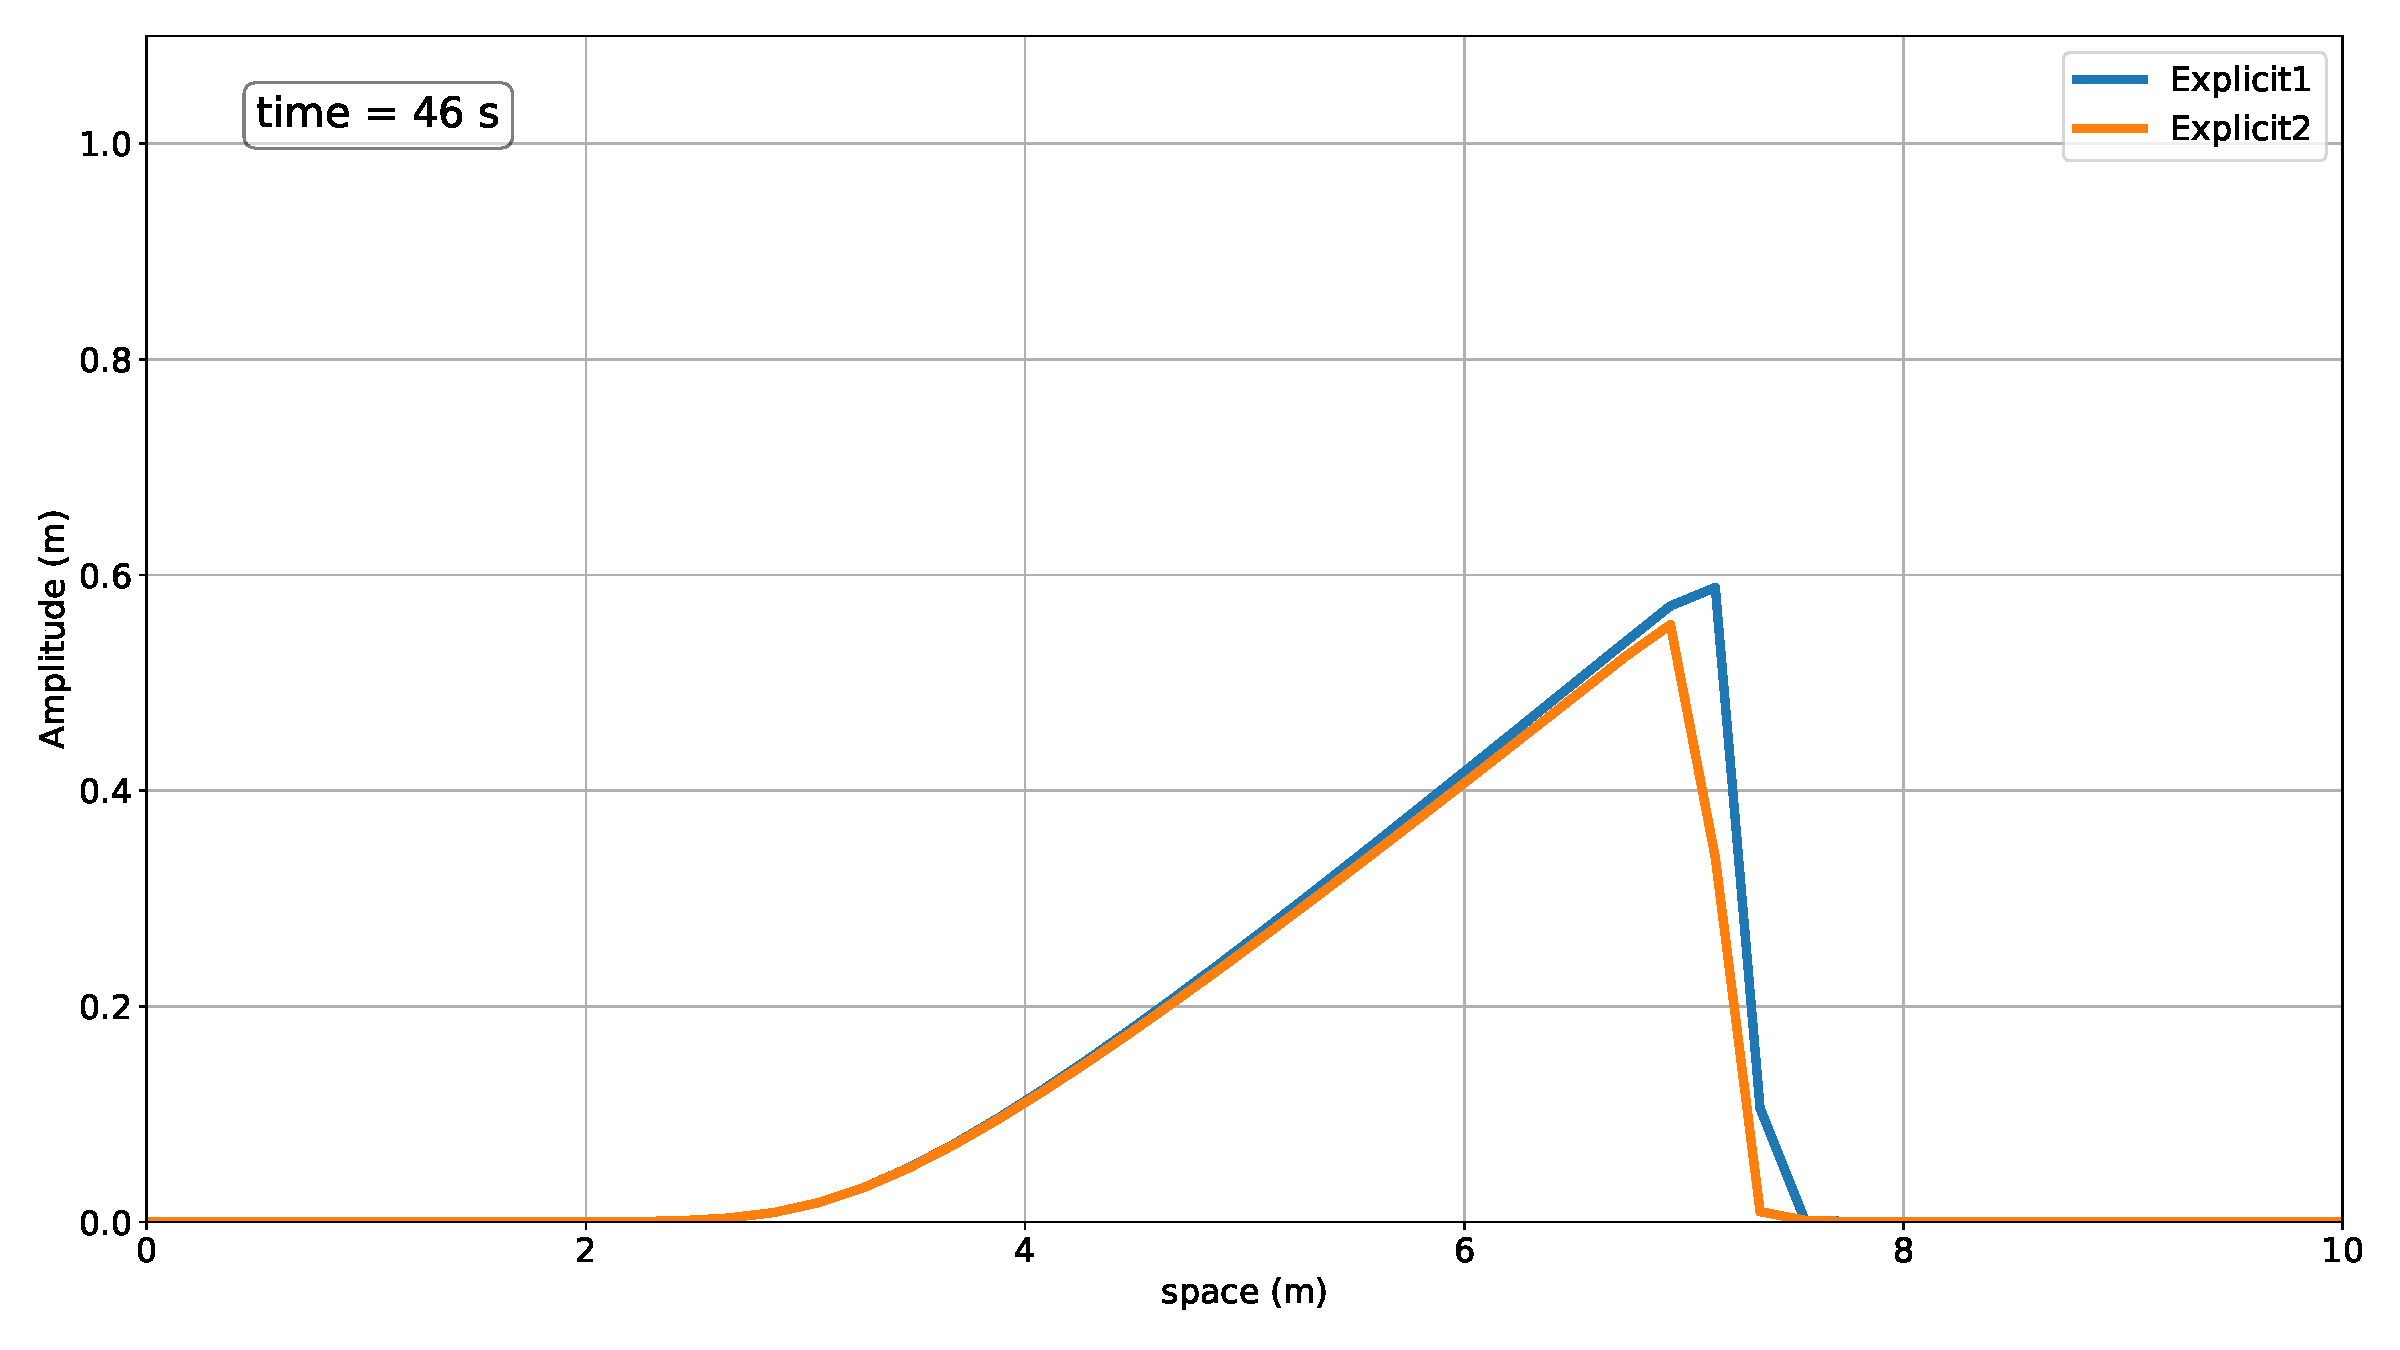
\includegraphics[width=\linewidth]{../BurgersEquation/images/expl9.pdf}
% 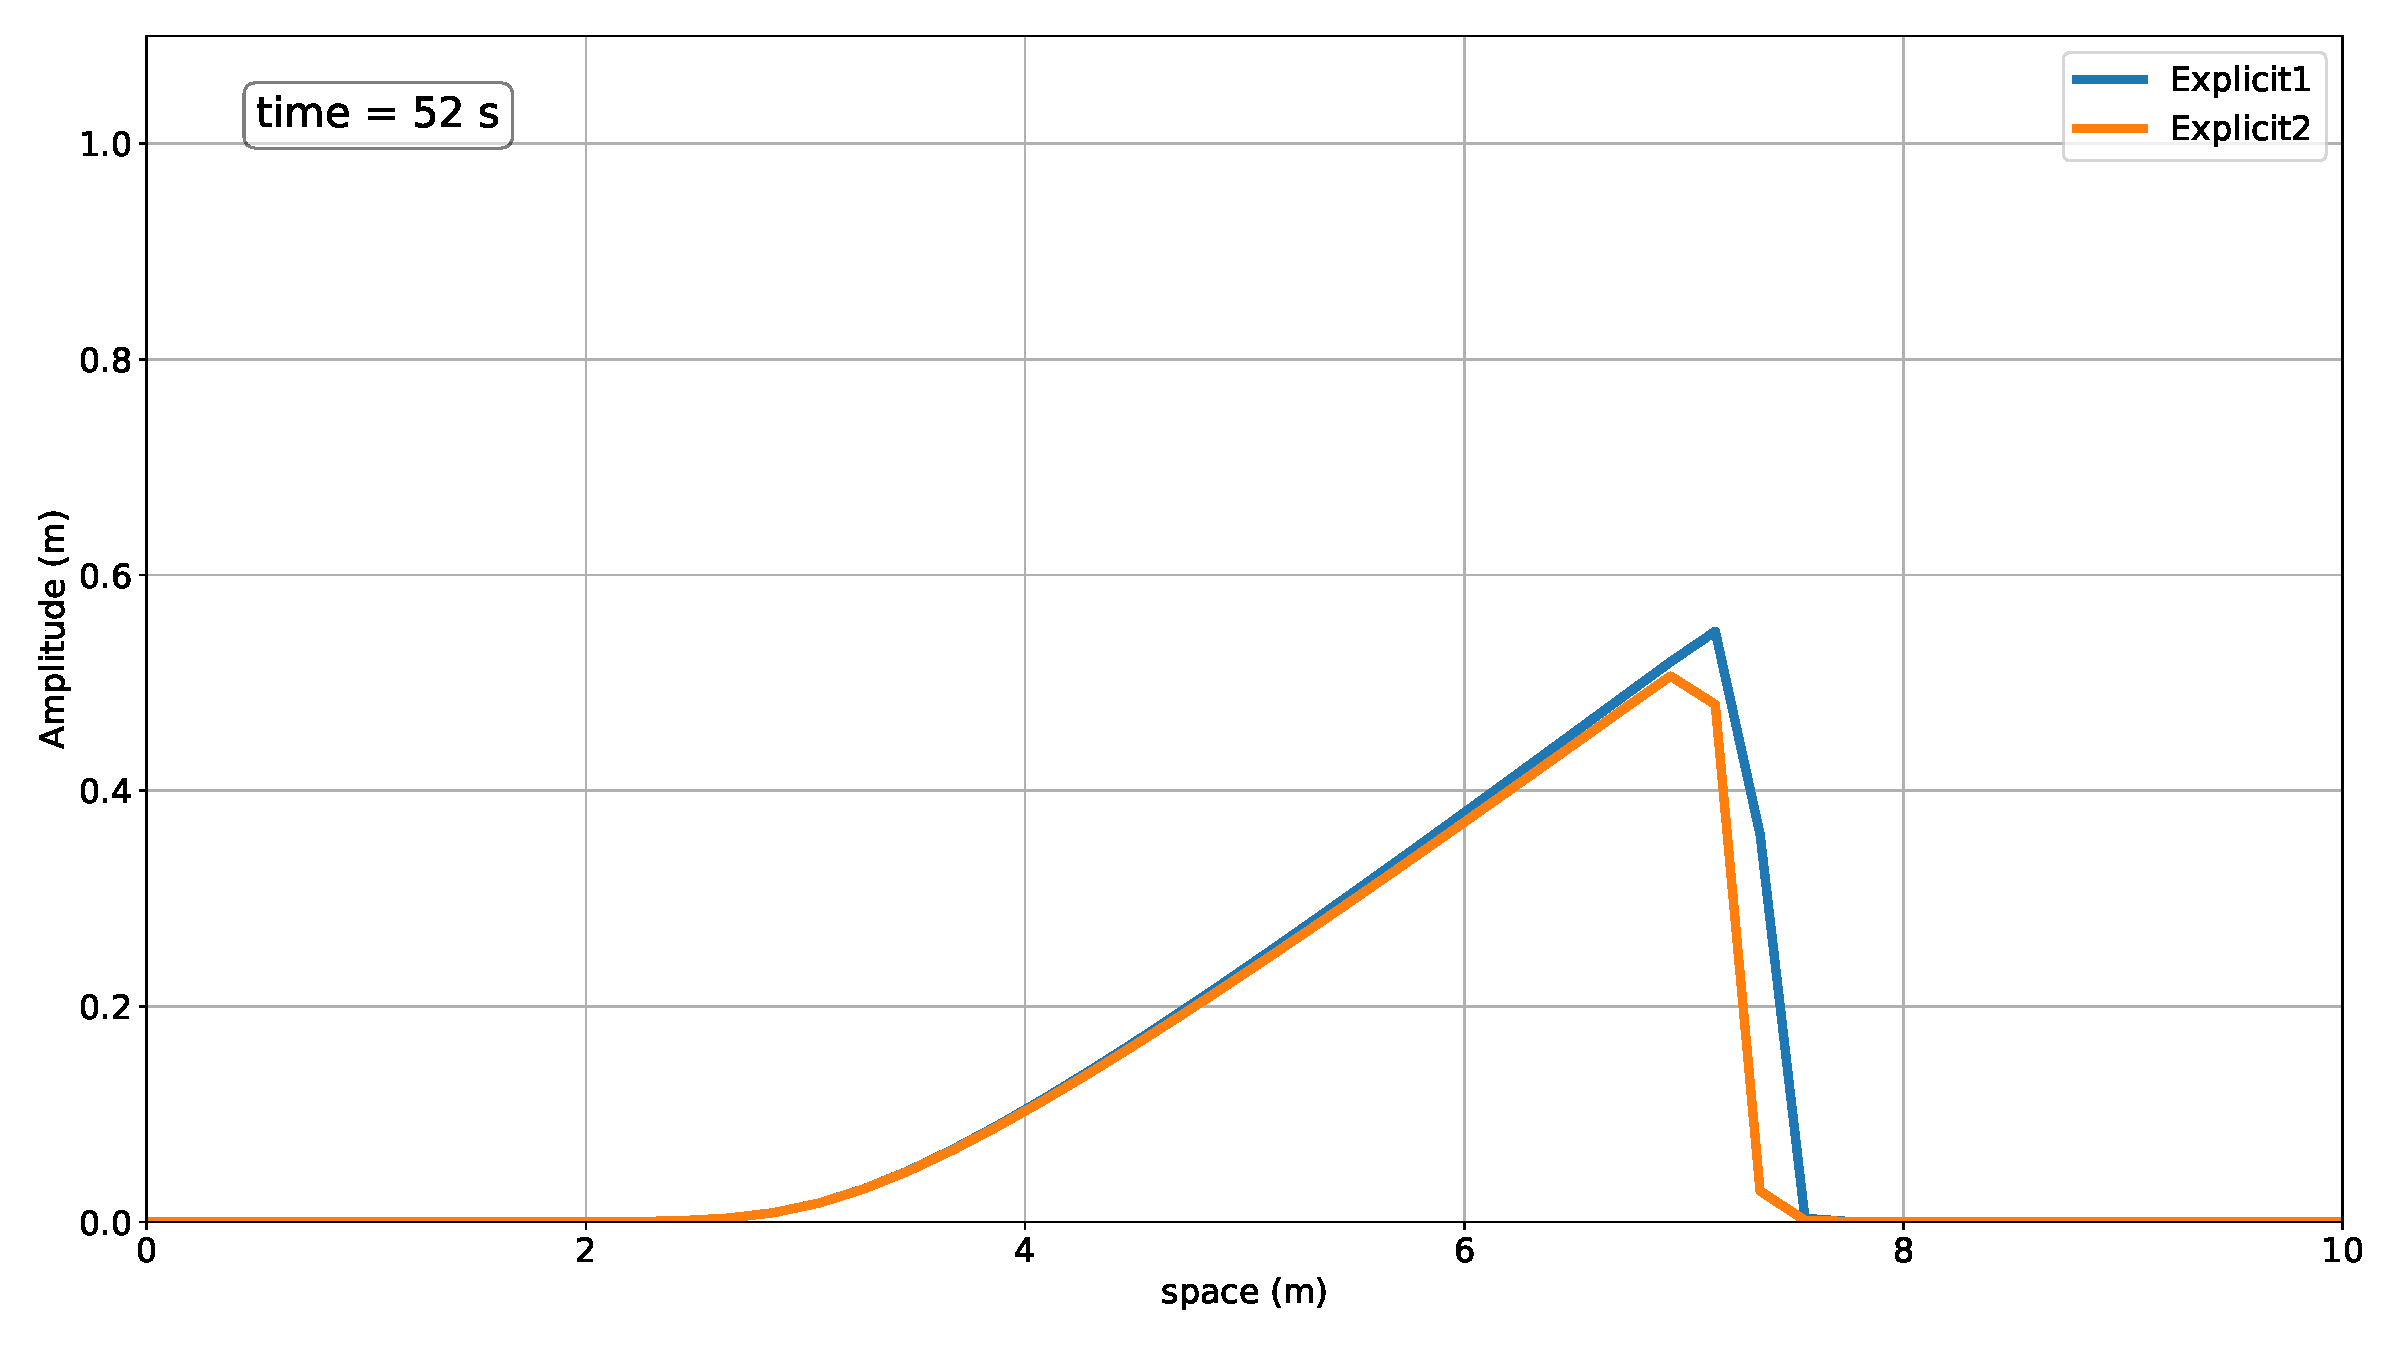
\includegraphics[width=\linewidth]{../BurgersEquation/images/expl10.pdf}
% 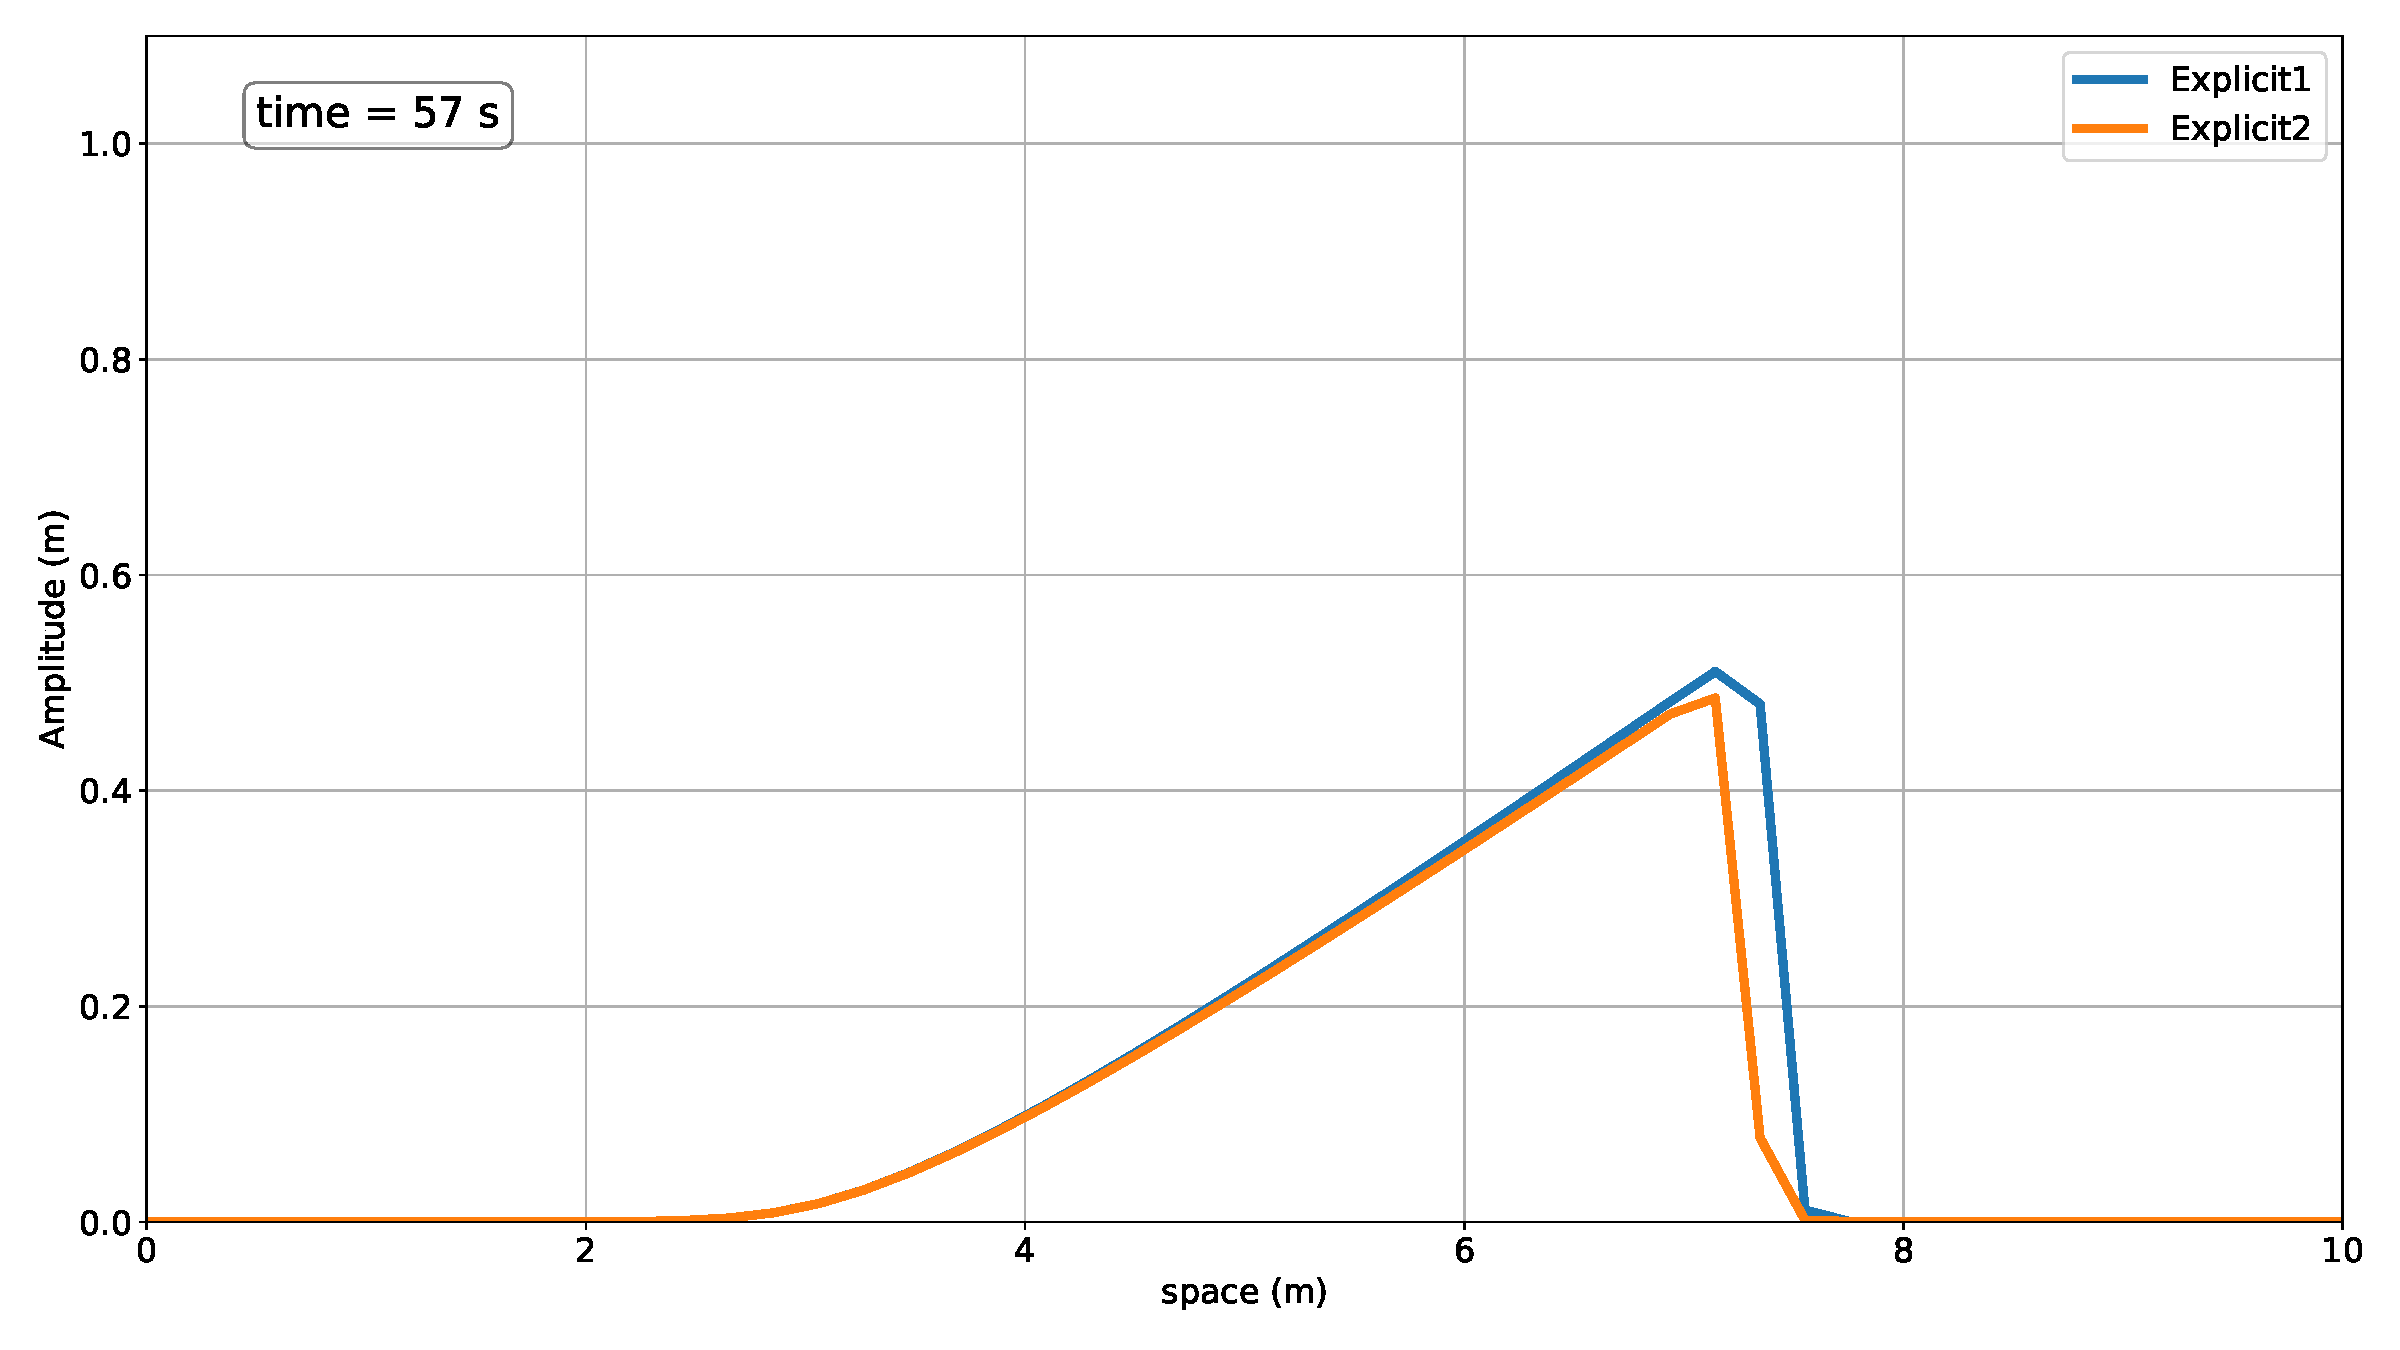
\includegraphics[width=\linewidth]{../BurgersEquation/images/expl11.pdf}
% 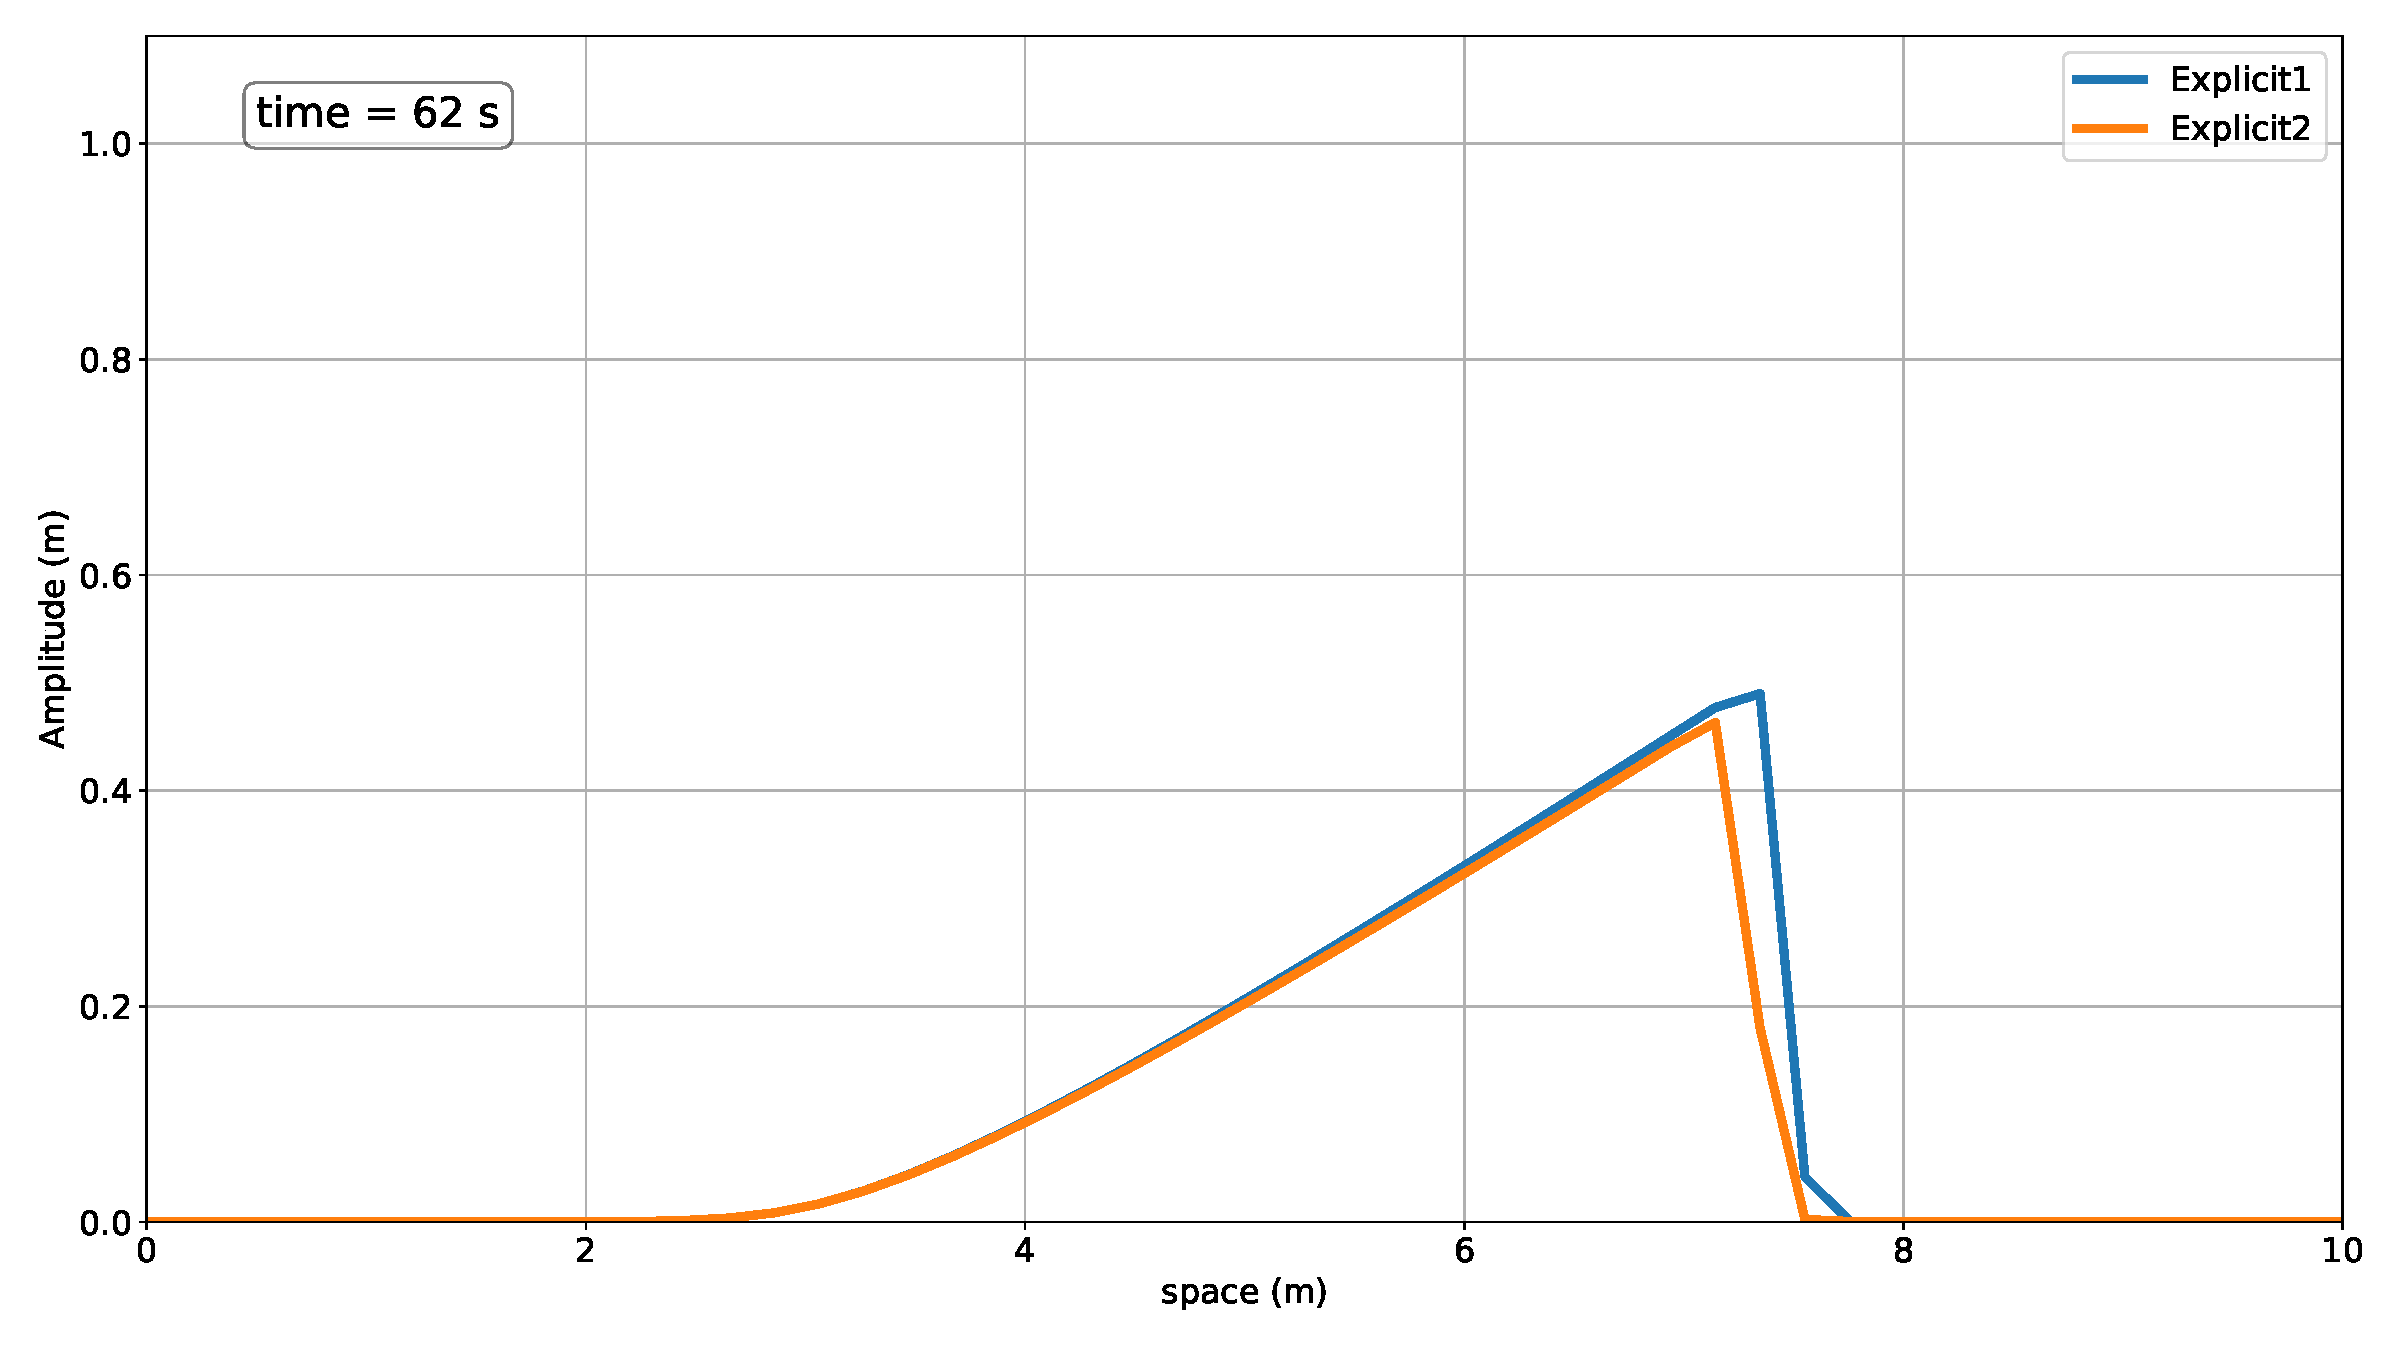
\includegraphics[width=\linewidth]{../BurgersEquation/images/expl12.pdf}
% 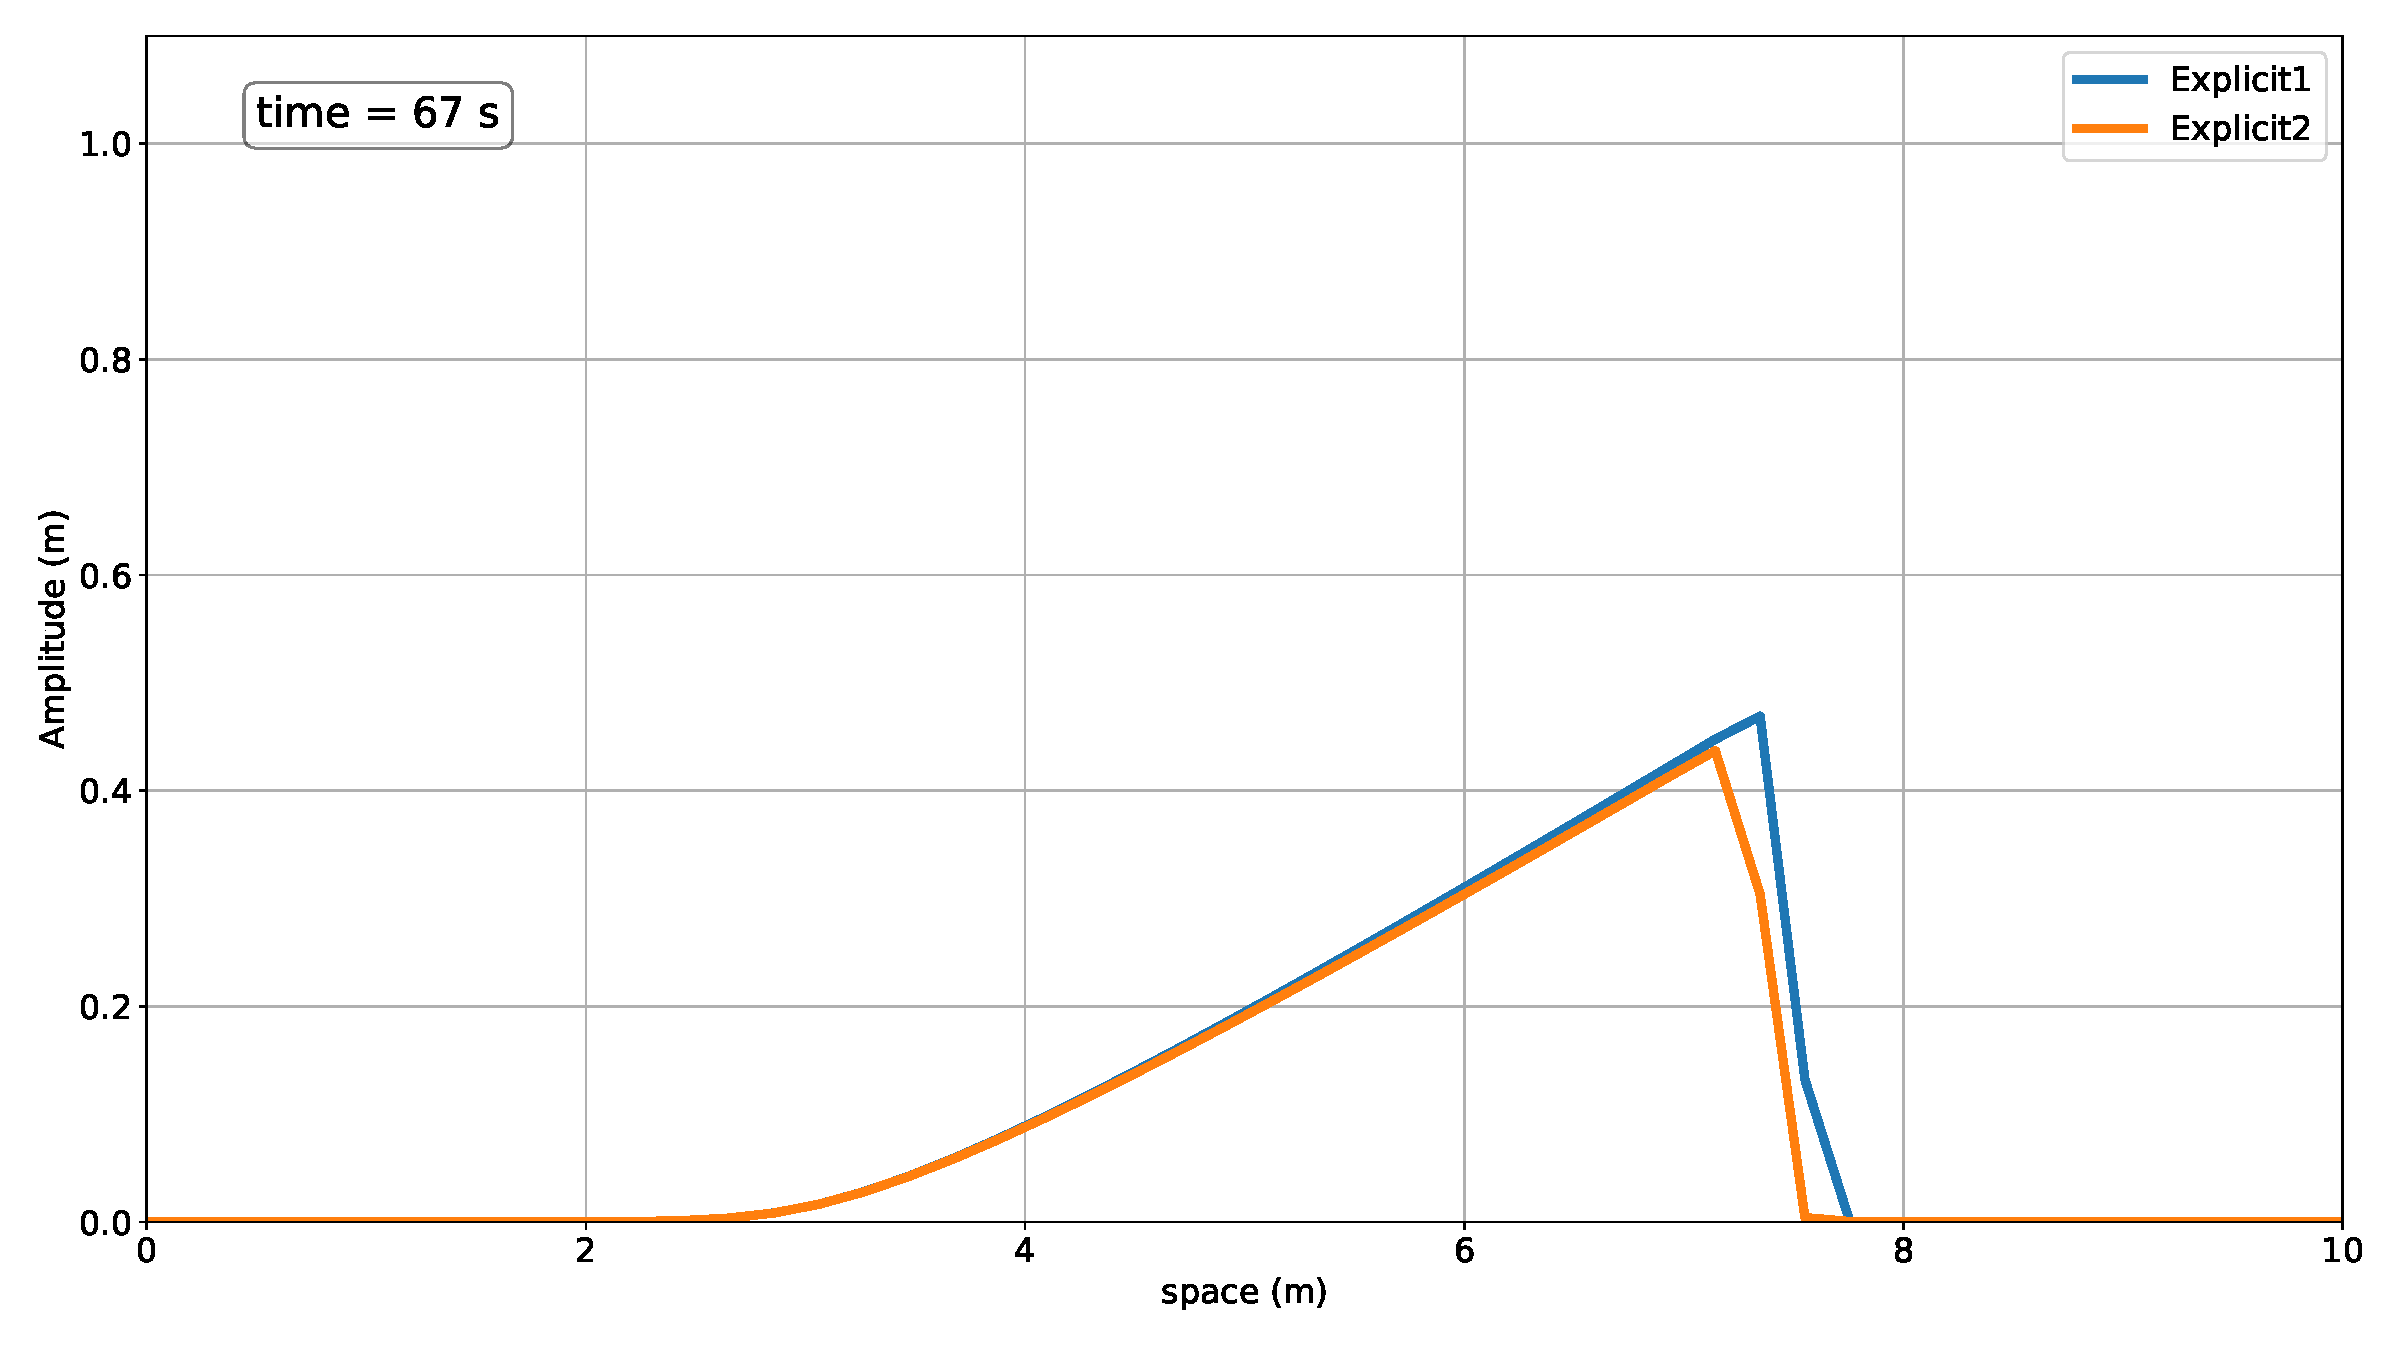
\includegraphics[width=\linewidth]{../BurgersEquation/images/expl13.pdf}
% 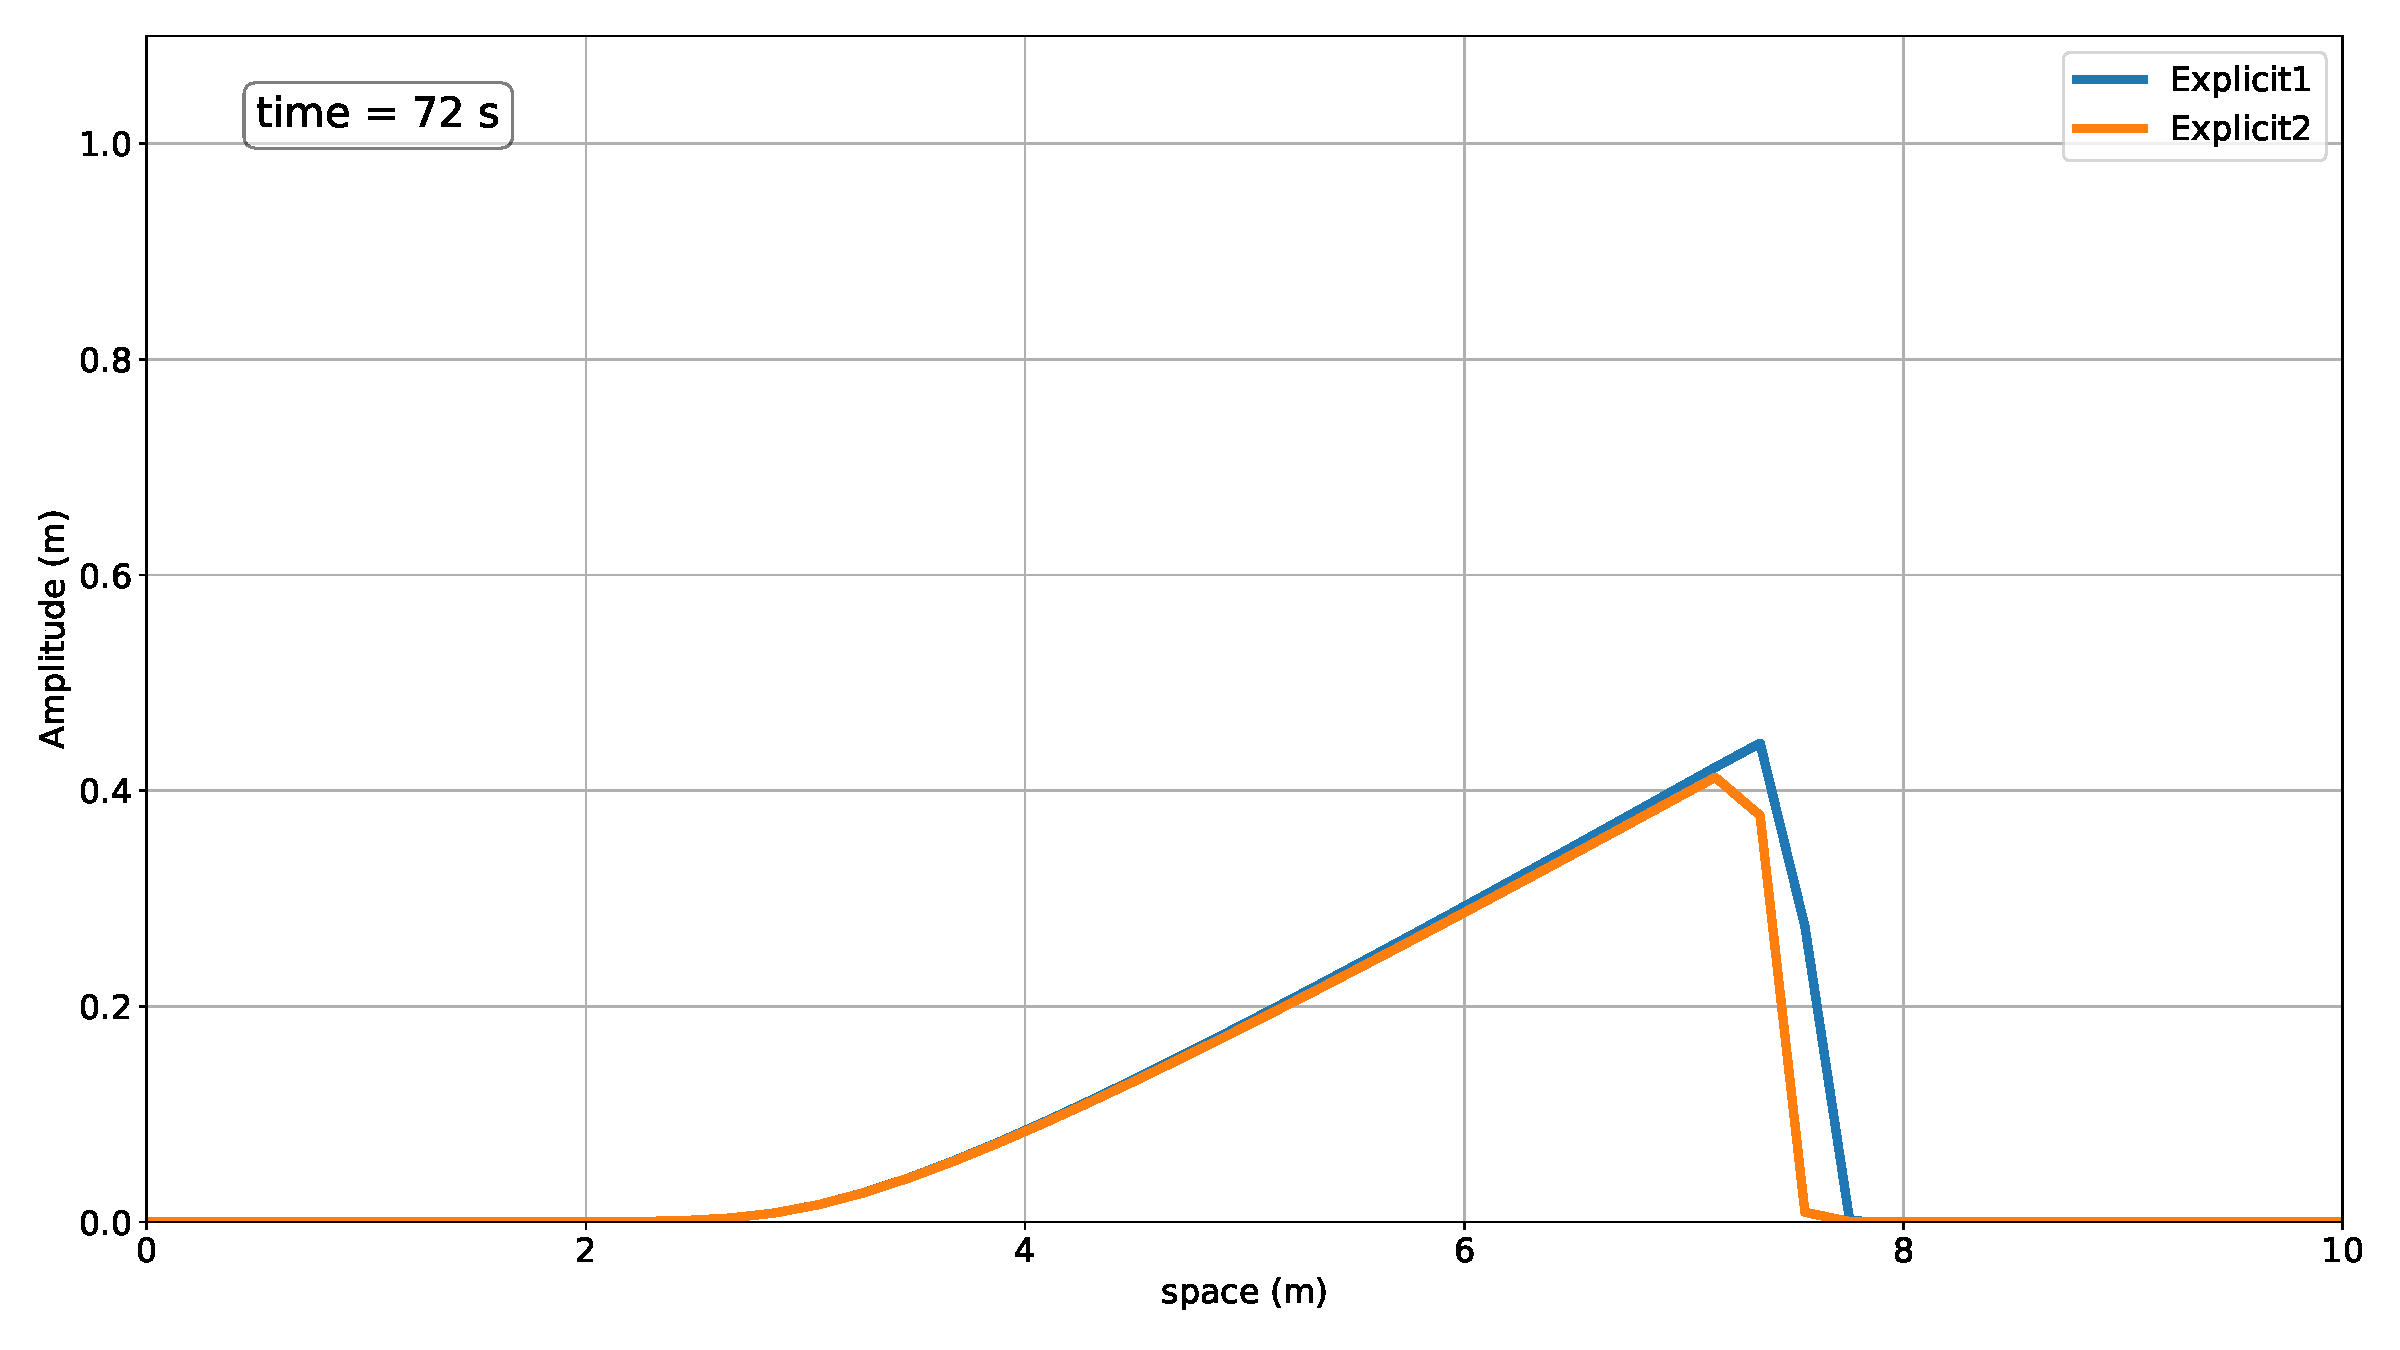
\includegraphics[width=\linewidth]{../BurgersEquation/images/expl14.pdf}
% 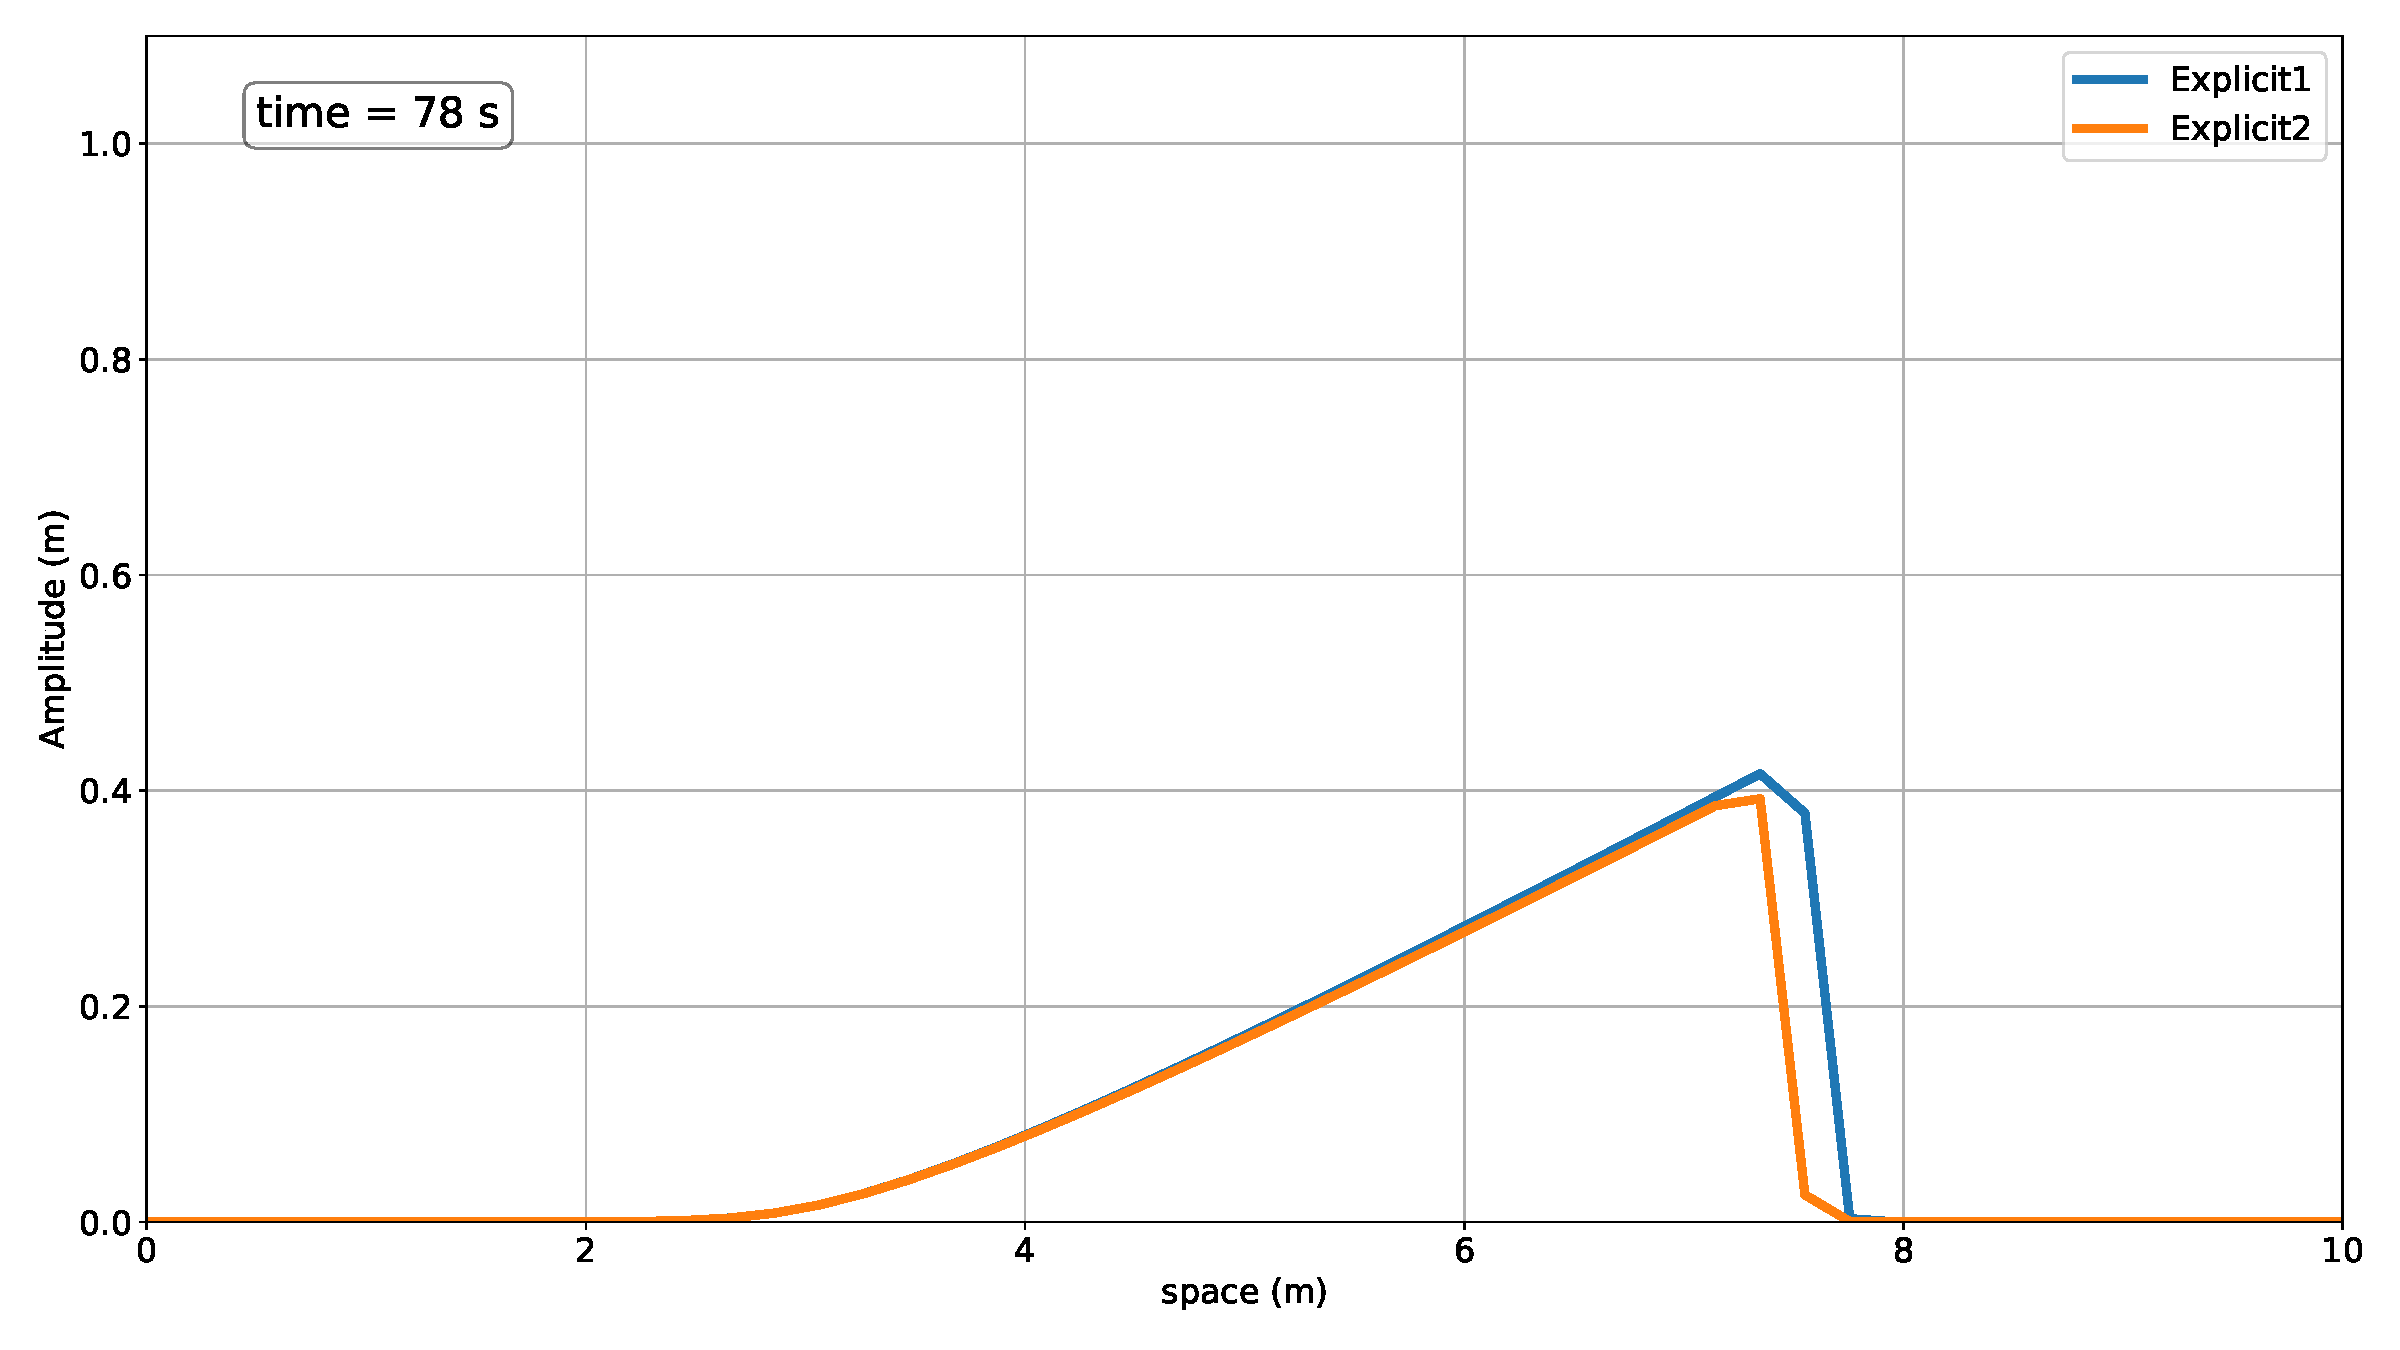
\includegraphics[width=\linewidth]{../BurgersEquation/images/expl15.pdf}
% 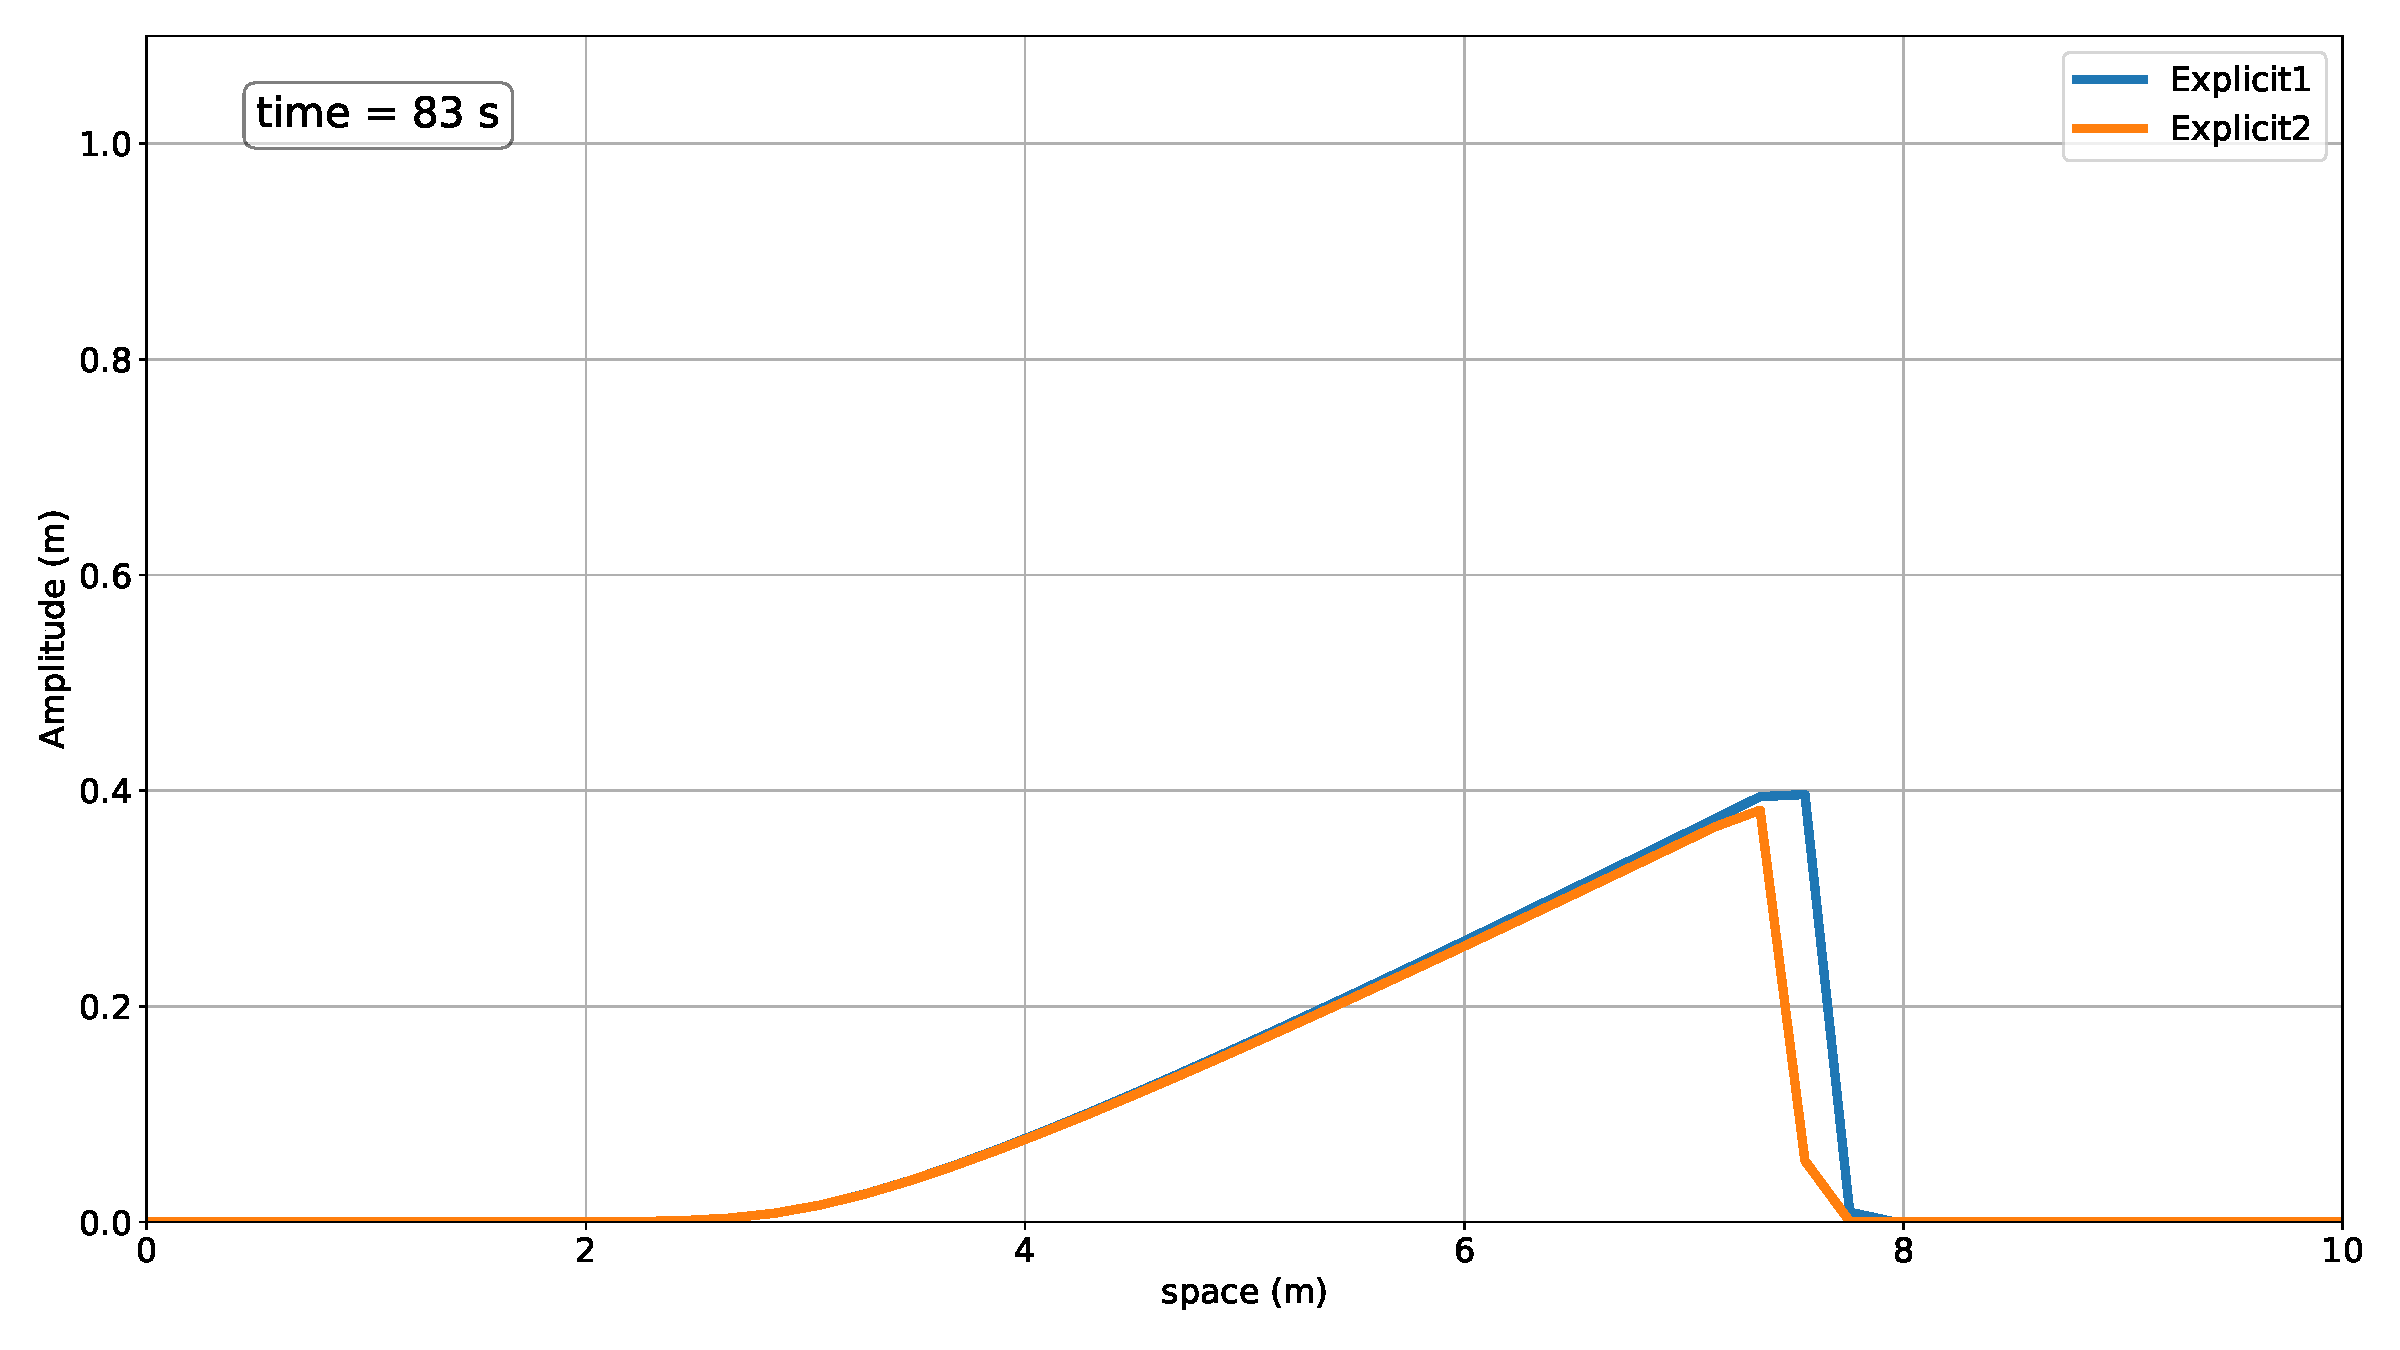
\includegraphics[width=\linewidth]{../BurgersEquation/images/expl16.pdf}
% 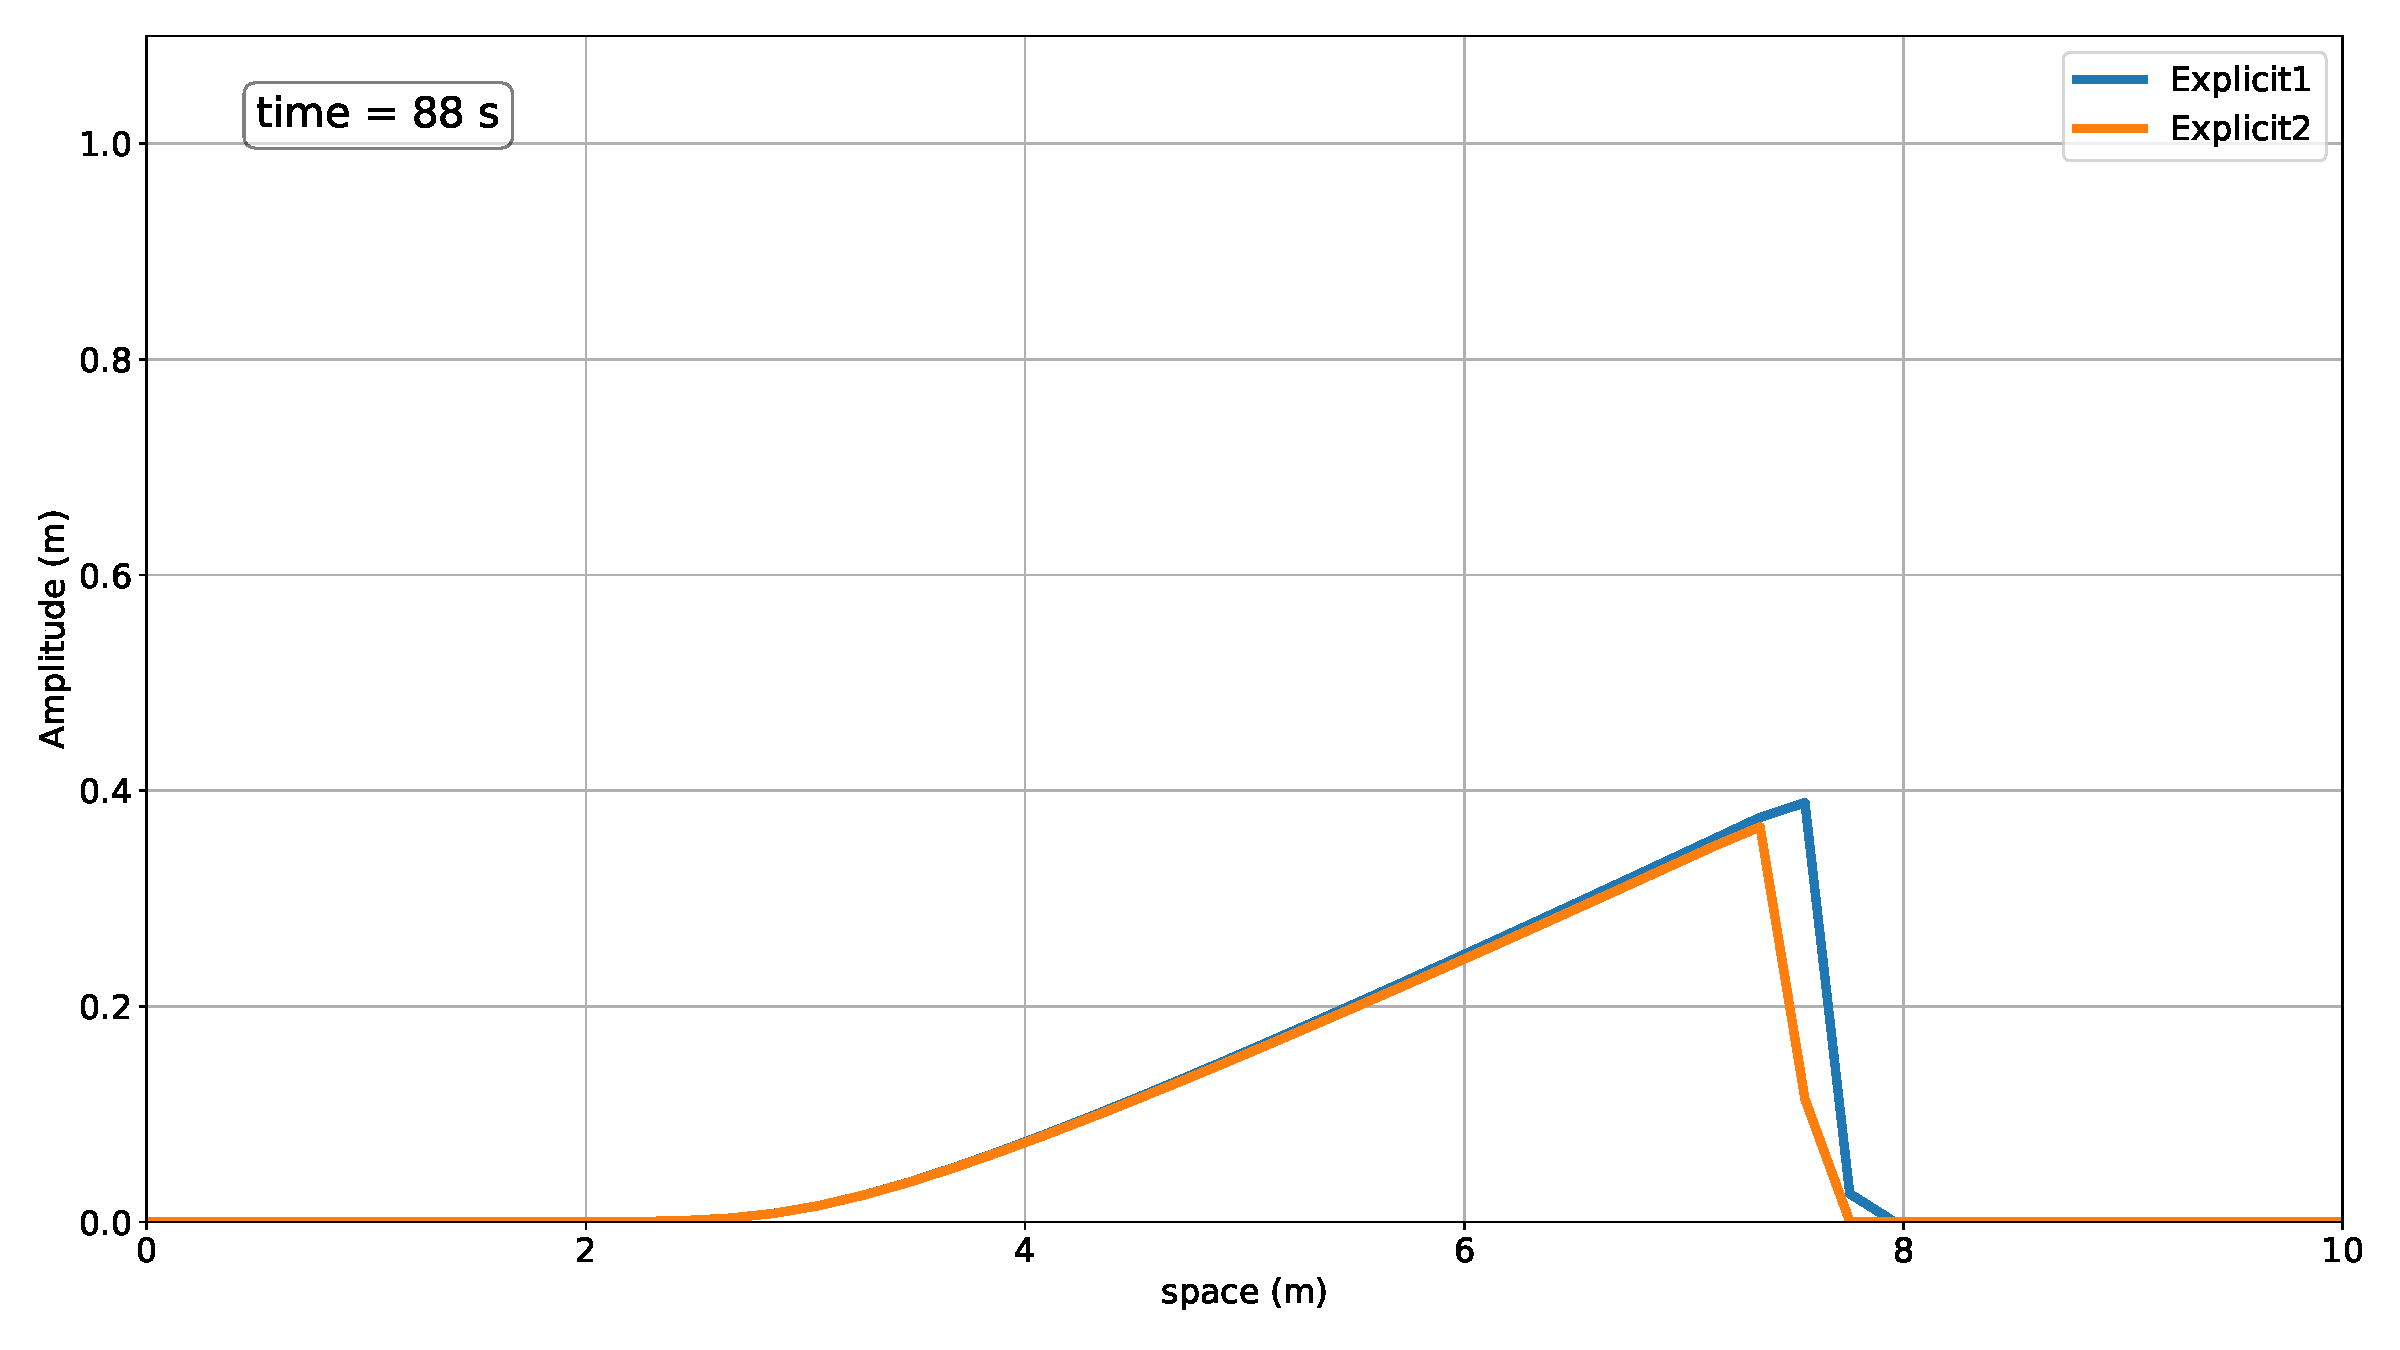
\includegraphics[width=\linewidth]{../BurgersEquation/images/expl17.pdf}
% 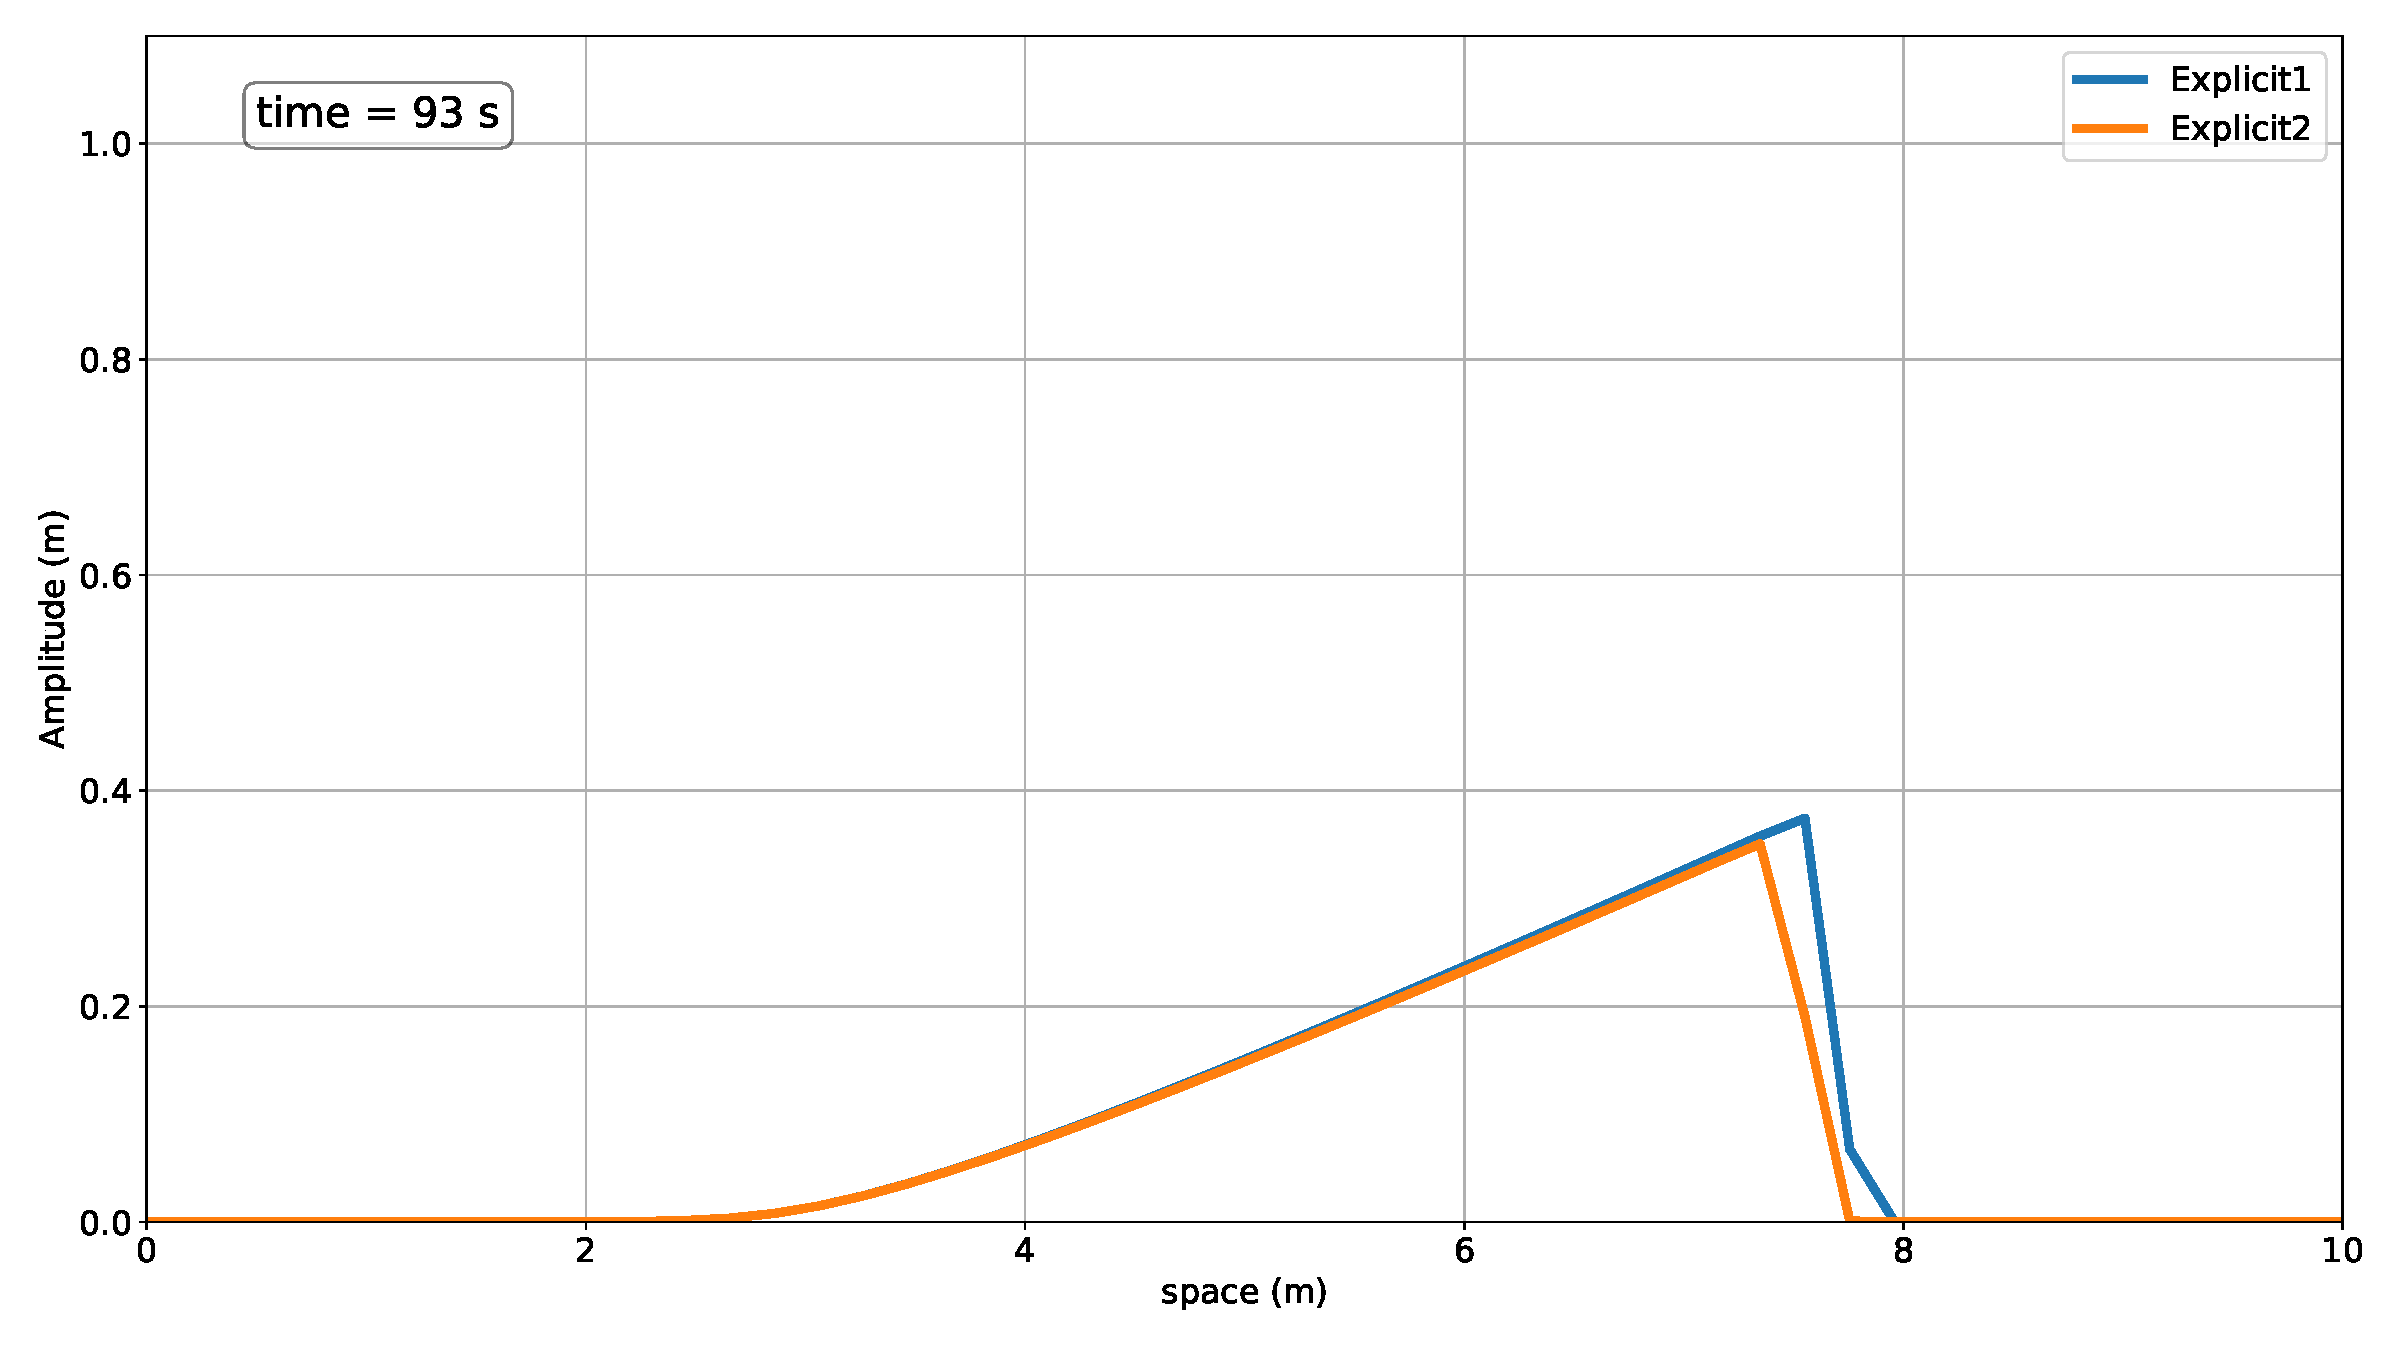
\includegraphics[width=\linewidth]{../BurgersEquation/images/expl18.pdf}
% 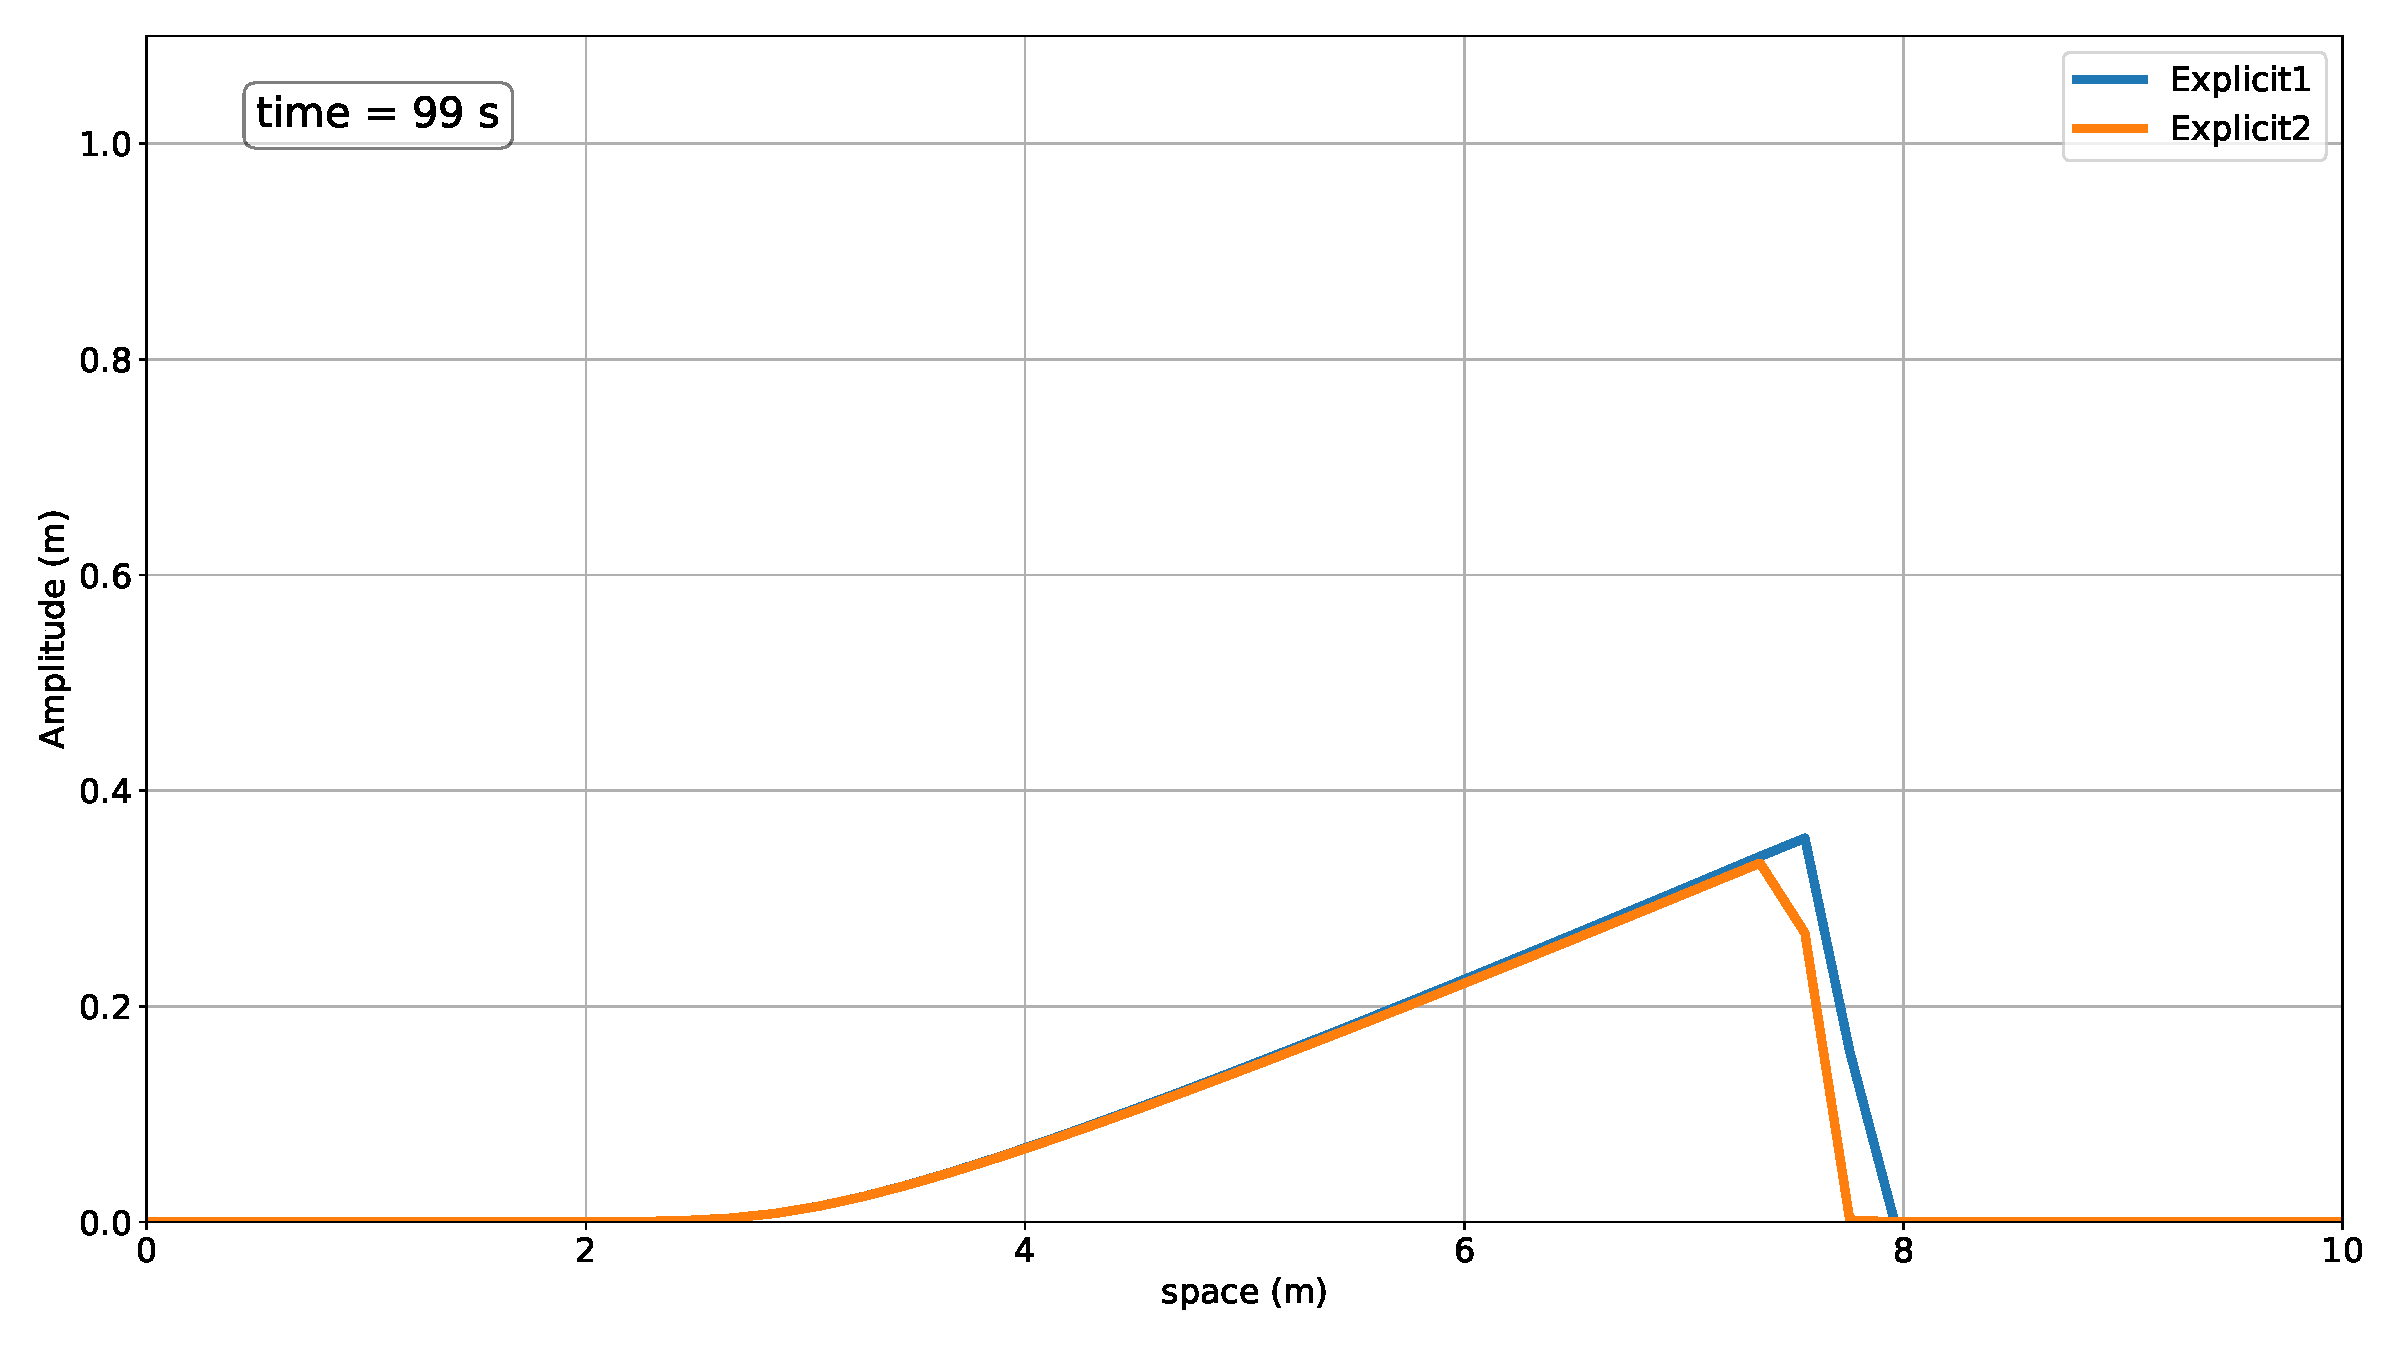
\includegraphics[width=\linewidth]{../BurgersEquation/images/expl19.pdf}





\begin{frame}
  \begin{columns}
    \column{0.5\linewidth}
    Euler forwards

  $$\frac{u_{i}^{n}-u_{i}^{n-1}}{\Delta t}+ u_{i}^{n-1}\, \frac{u_{i+1}^{n-1}-u_{i-1}^{n-1}}{2\,\Delta x}=0$$
  $$ u_{i}^{n} = \frac{u^{n-1}_{i}\, \left(- \Delta{t}\, u^{n-1}_{i+1}\, + \Delta{t}\, u^{n-1}_{i-1}\, + 2 \Delta{x}\,\right)}{2 \Delta{x}\,}$$
    \column{0.5\linewidth}
    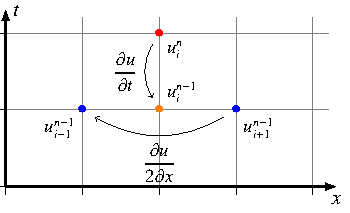
\includegraphics[width=\linewidth]{../BurgersEquation/tikz/linear3/linear3.pdf}\\
  \end{columns}
\end{frame}

\begin{frame}
  \begin{columns}
    \column{0.5\linewidth}
    Euler forwards

  $$\frac{u_{i}^{n}-u_{i}^{n-1}}{\Delta t}+ u_{i}^{n}\, \frac{u_{i+1}^{n-1}-u_{i-1}^{n-1}}{2\,\Delta x}=0$$
  $$ u_{i}^{n} = \frac{2 \Delta{x}\, u^{n-1}_{i}\,}{\Delta{t}\, u^{n-1}_{i+1}\, - \Delta{t}\, u^{n-1}_{i-1}\, + 2 \Delta{x}\,}$$
    \column{0.5\linewidth}
    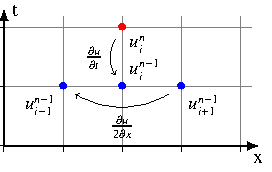
\includegraphics[width=\linewidth]{../BurgersEquation/tikz/linear4/linear4.pdf}\\
  \end{columns}
\end{frame}

% 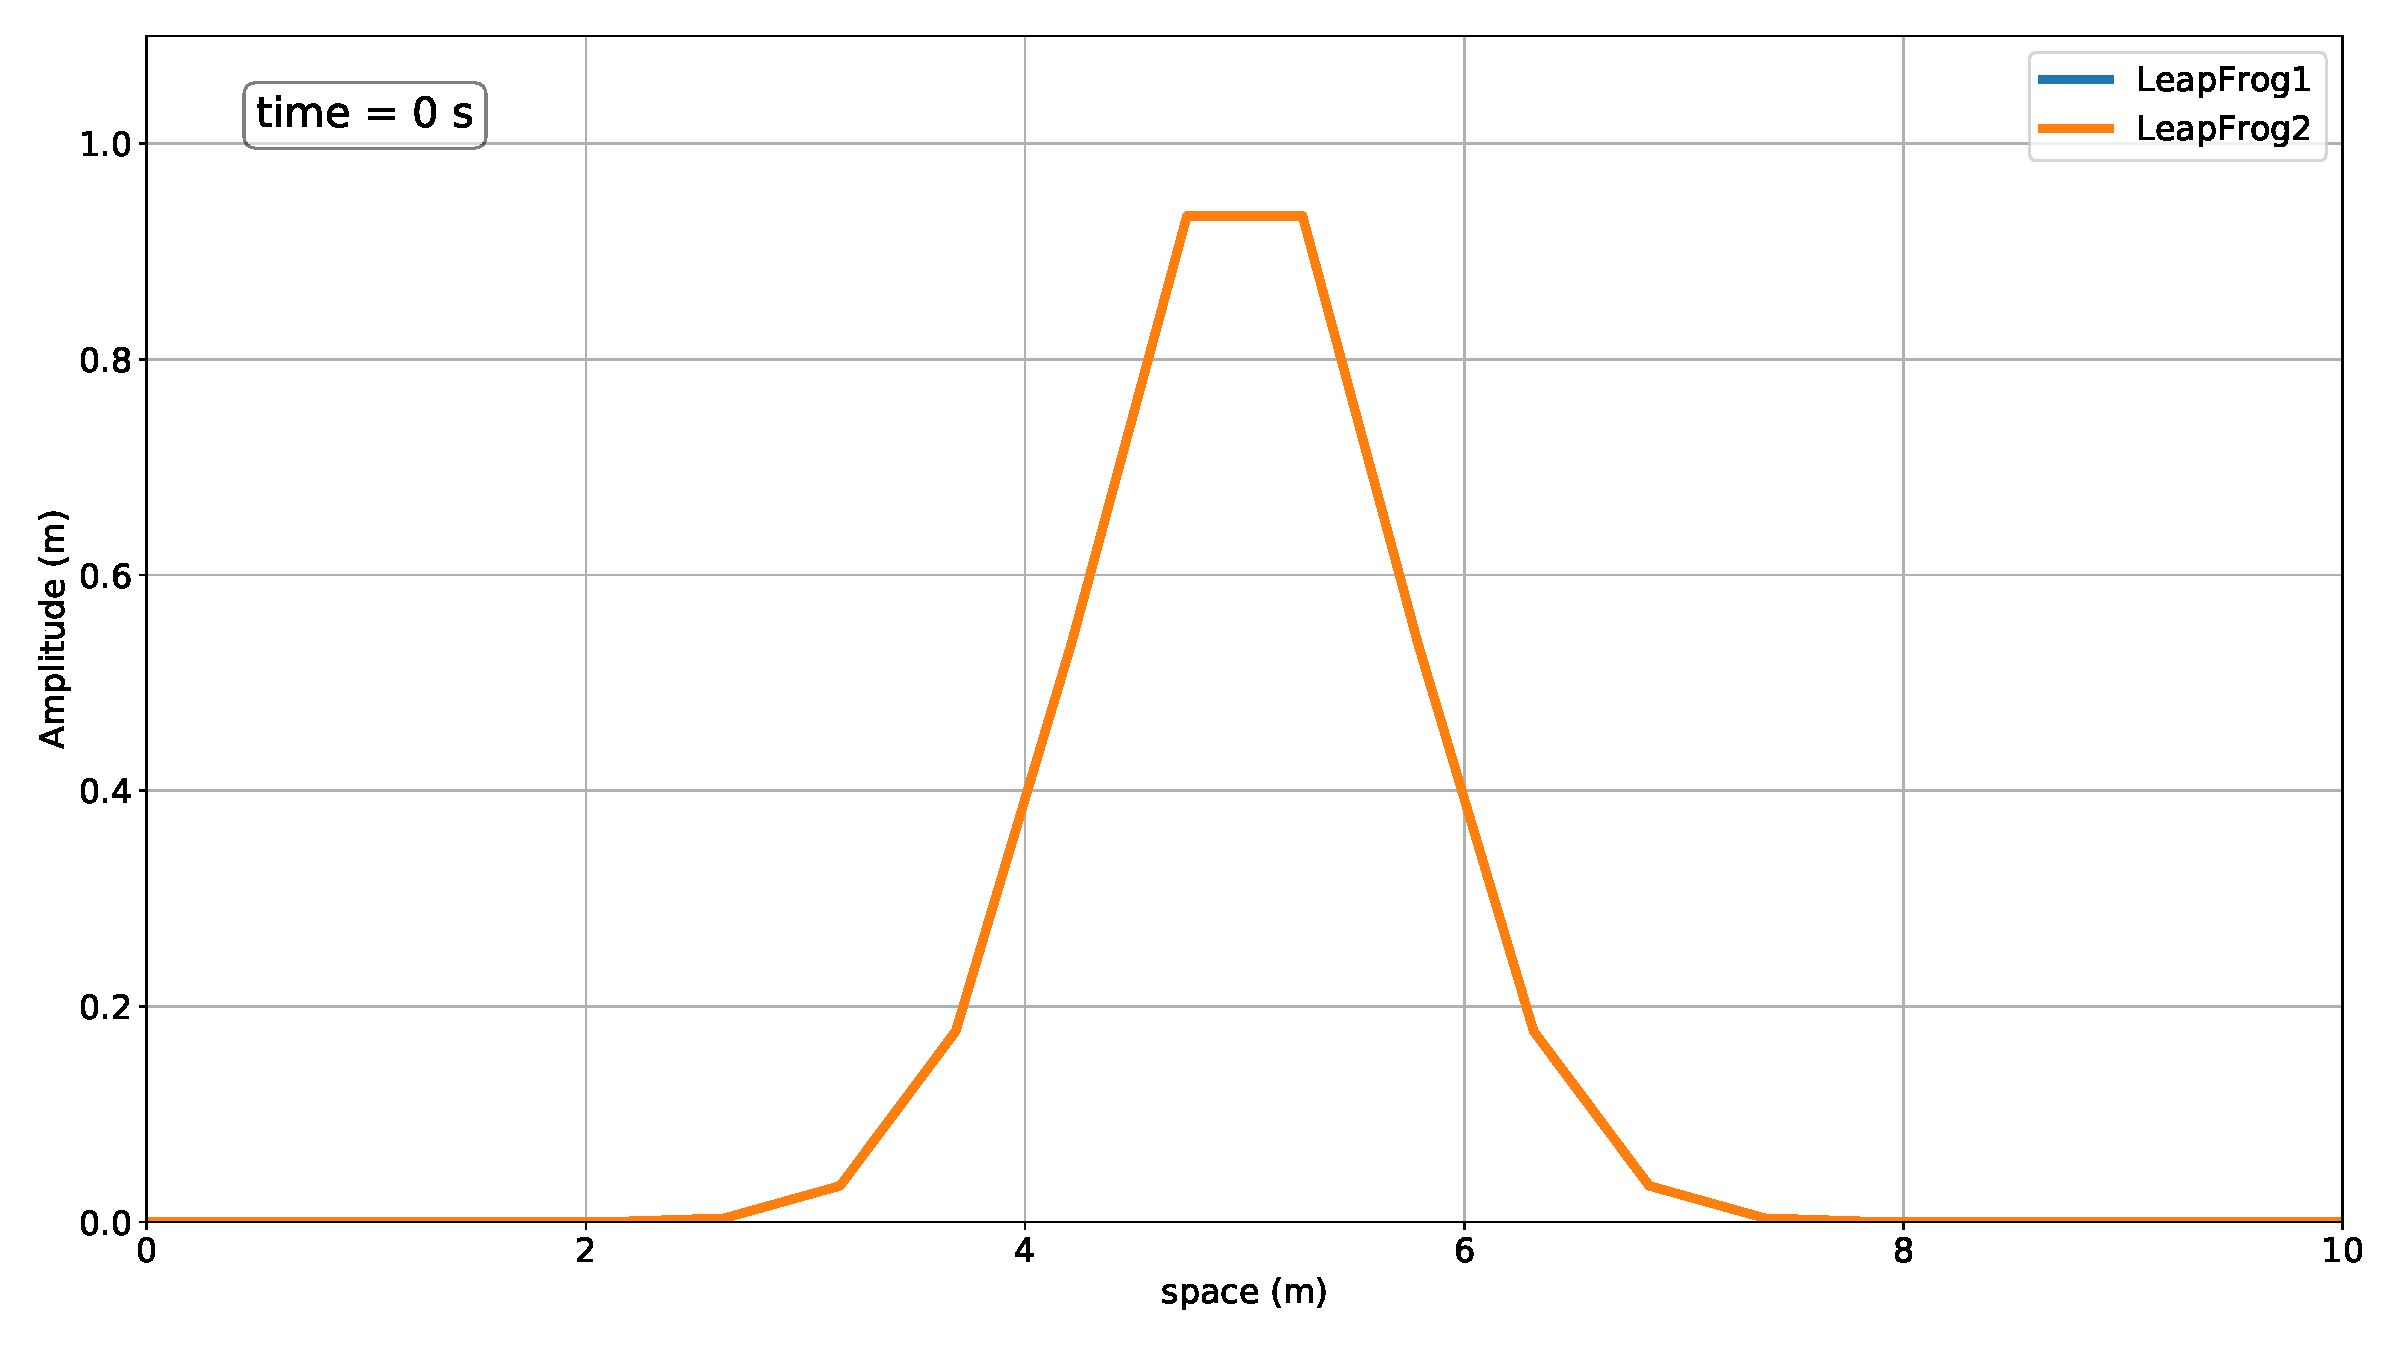
\includegraphics[width=\linewidth]{../BurgersEquation/images/Lin3_Lin40.pdf}
% 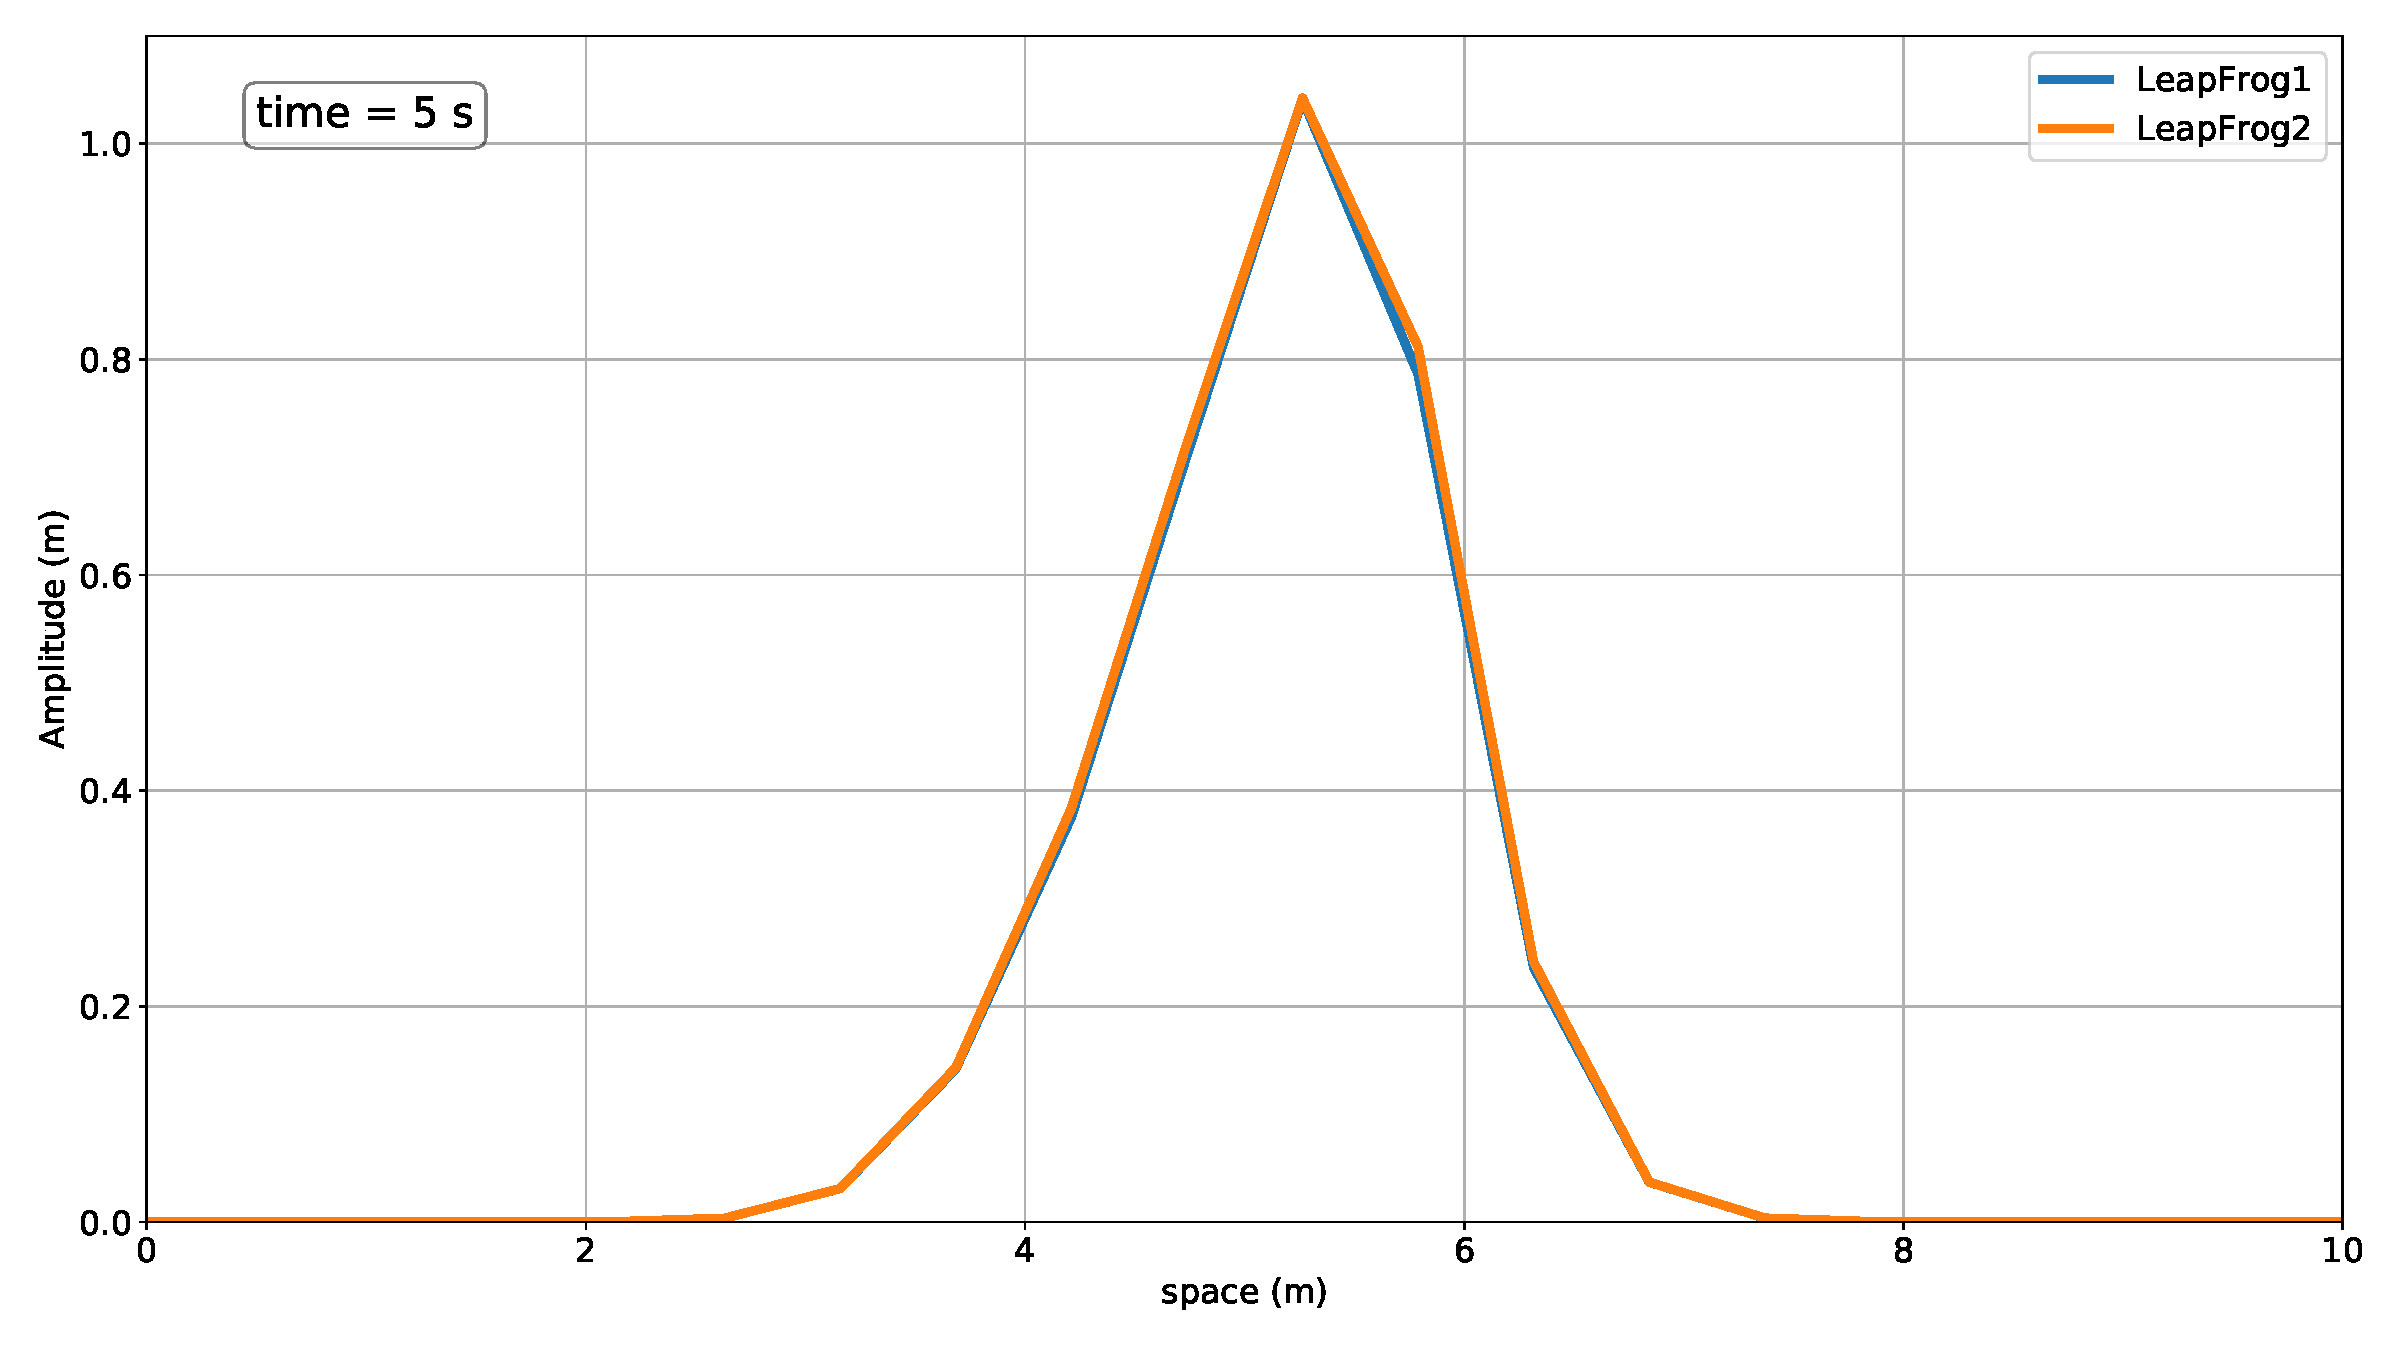
\includegraphics[width=\linewidth]{../BurgersEquation/images/Lin3_Lin41.pdf}
% 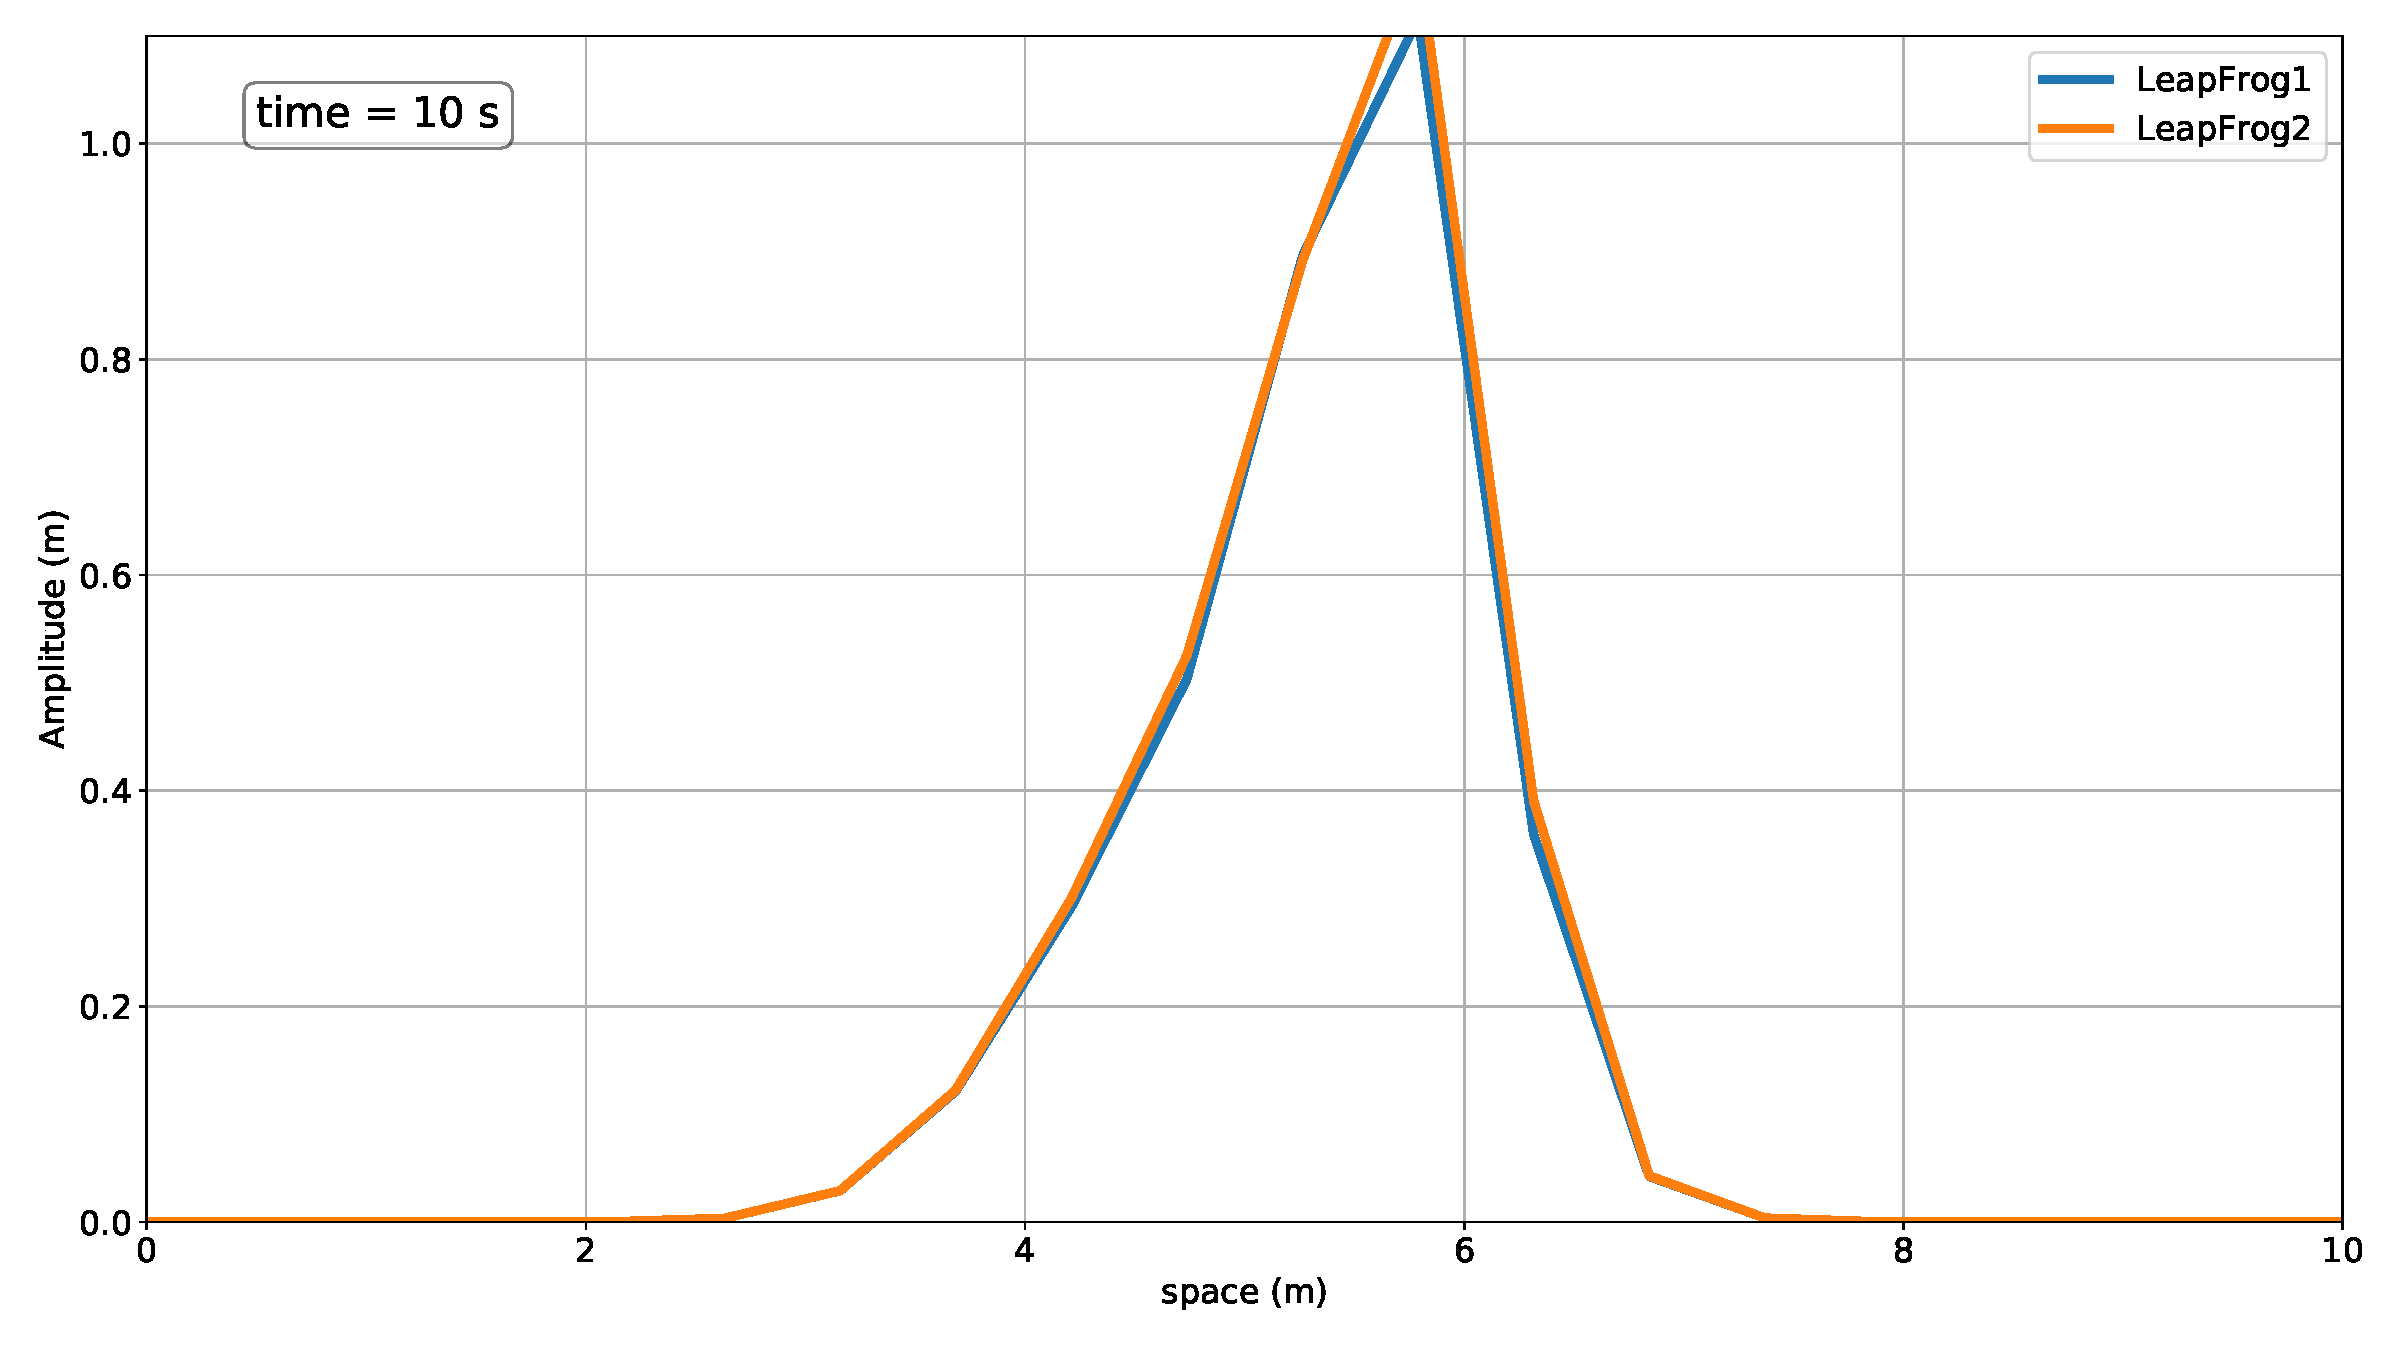
\includegraphics[width=\linewidth]{../BurgersEquation/images/Lin3_Lin42.pdf}
% 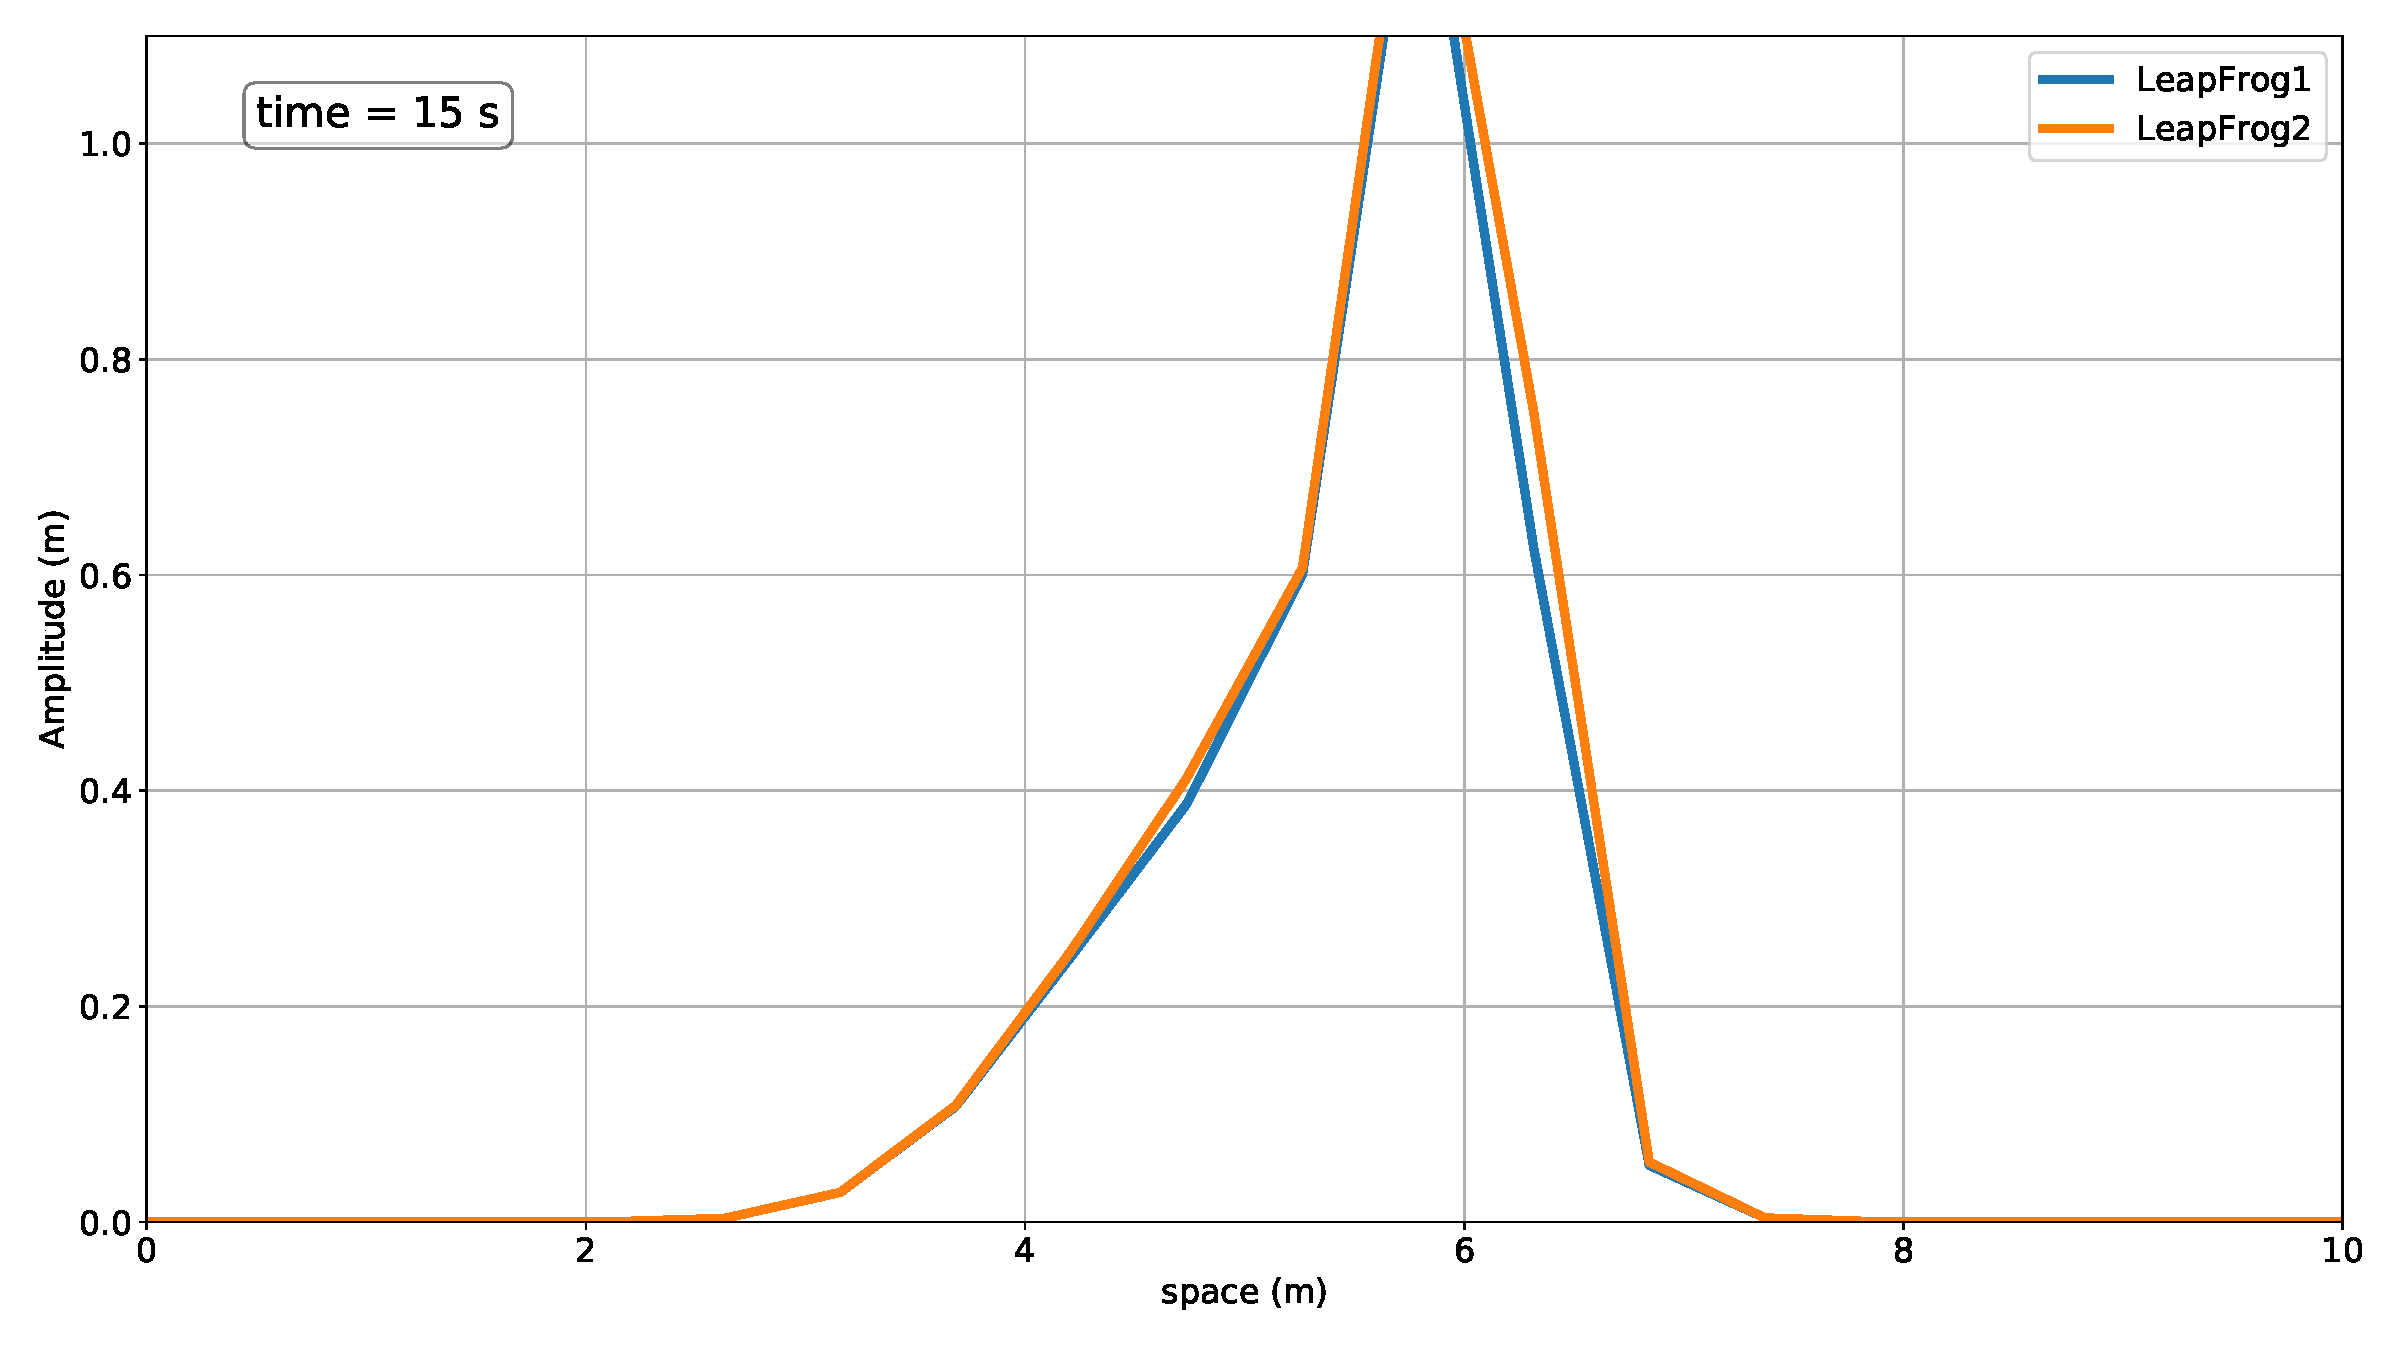
\includegraphics[width=\linewidth]{../BurgersEquation/images/Lin3_Lin43.pdf}
% 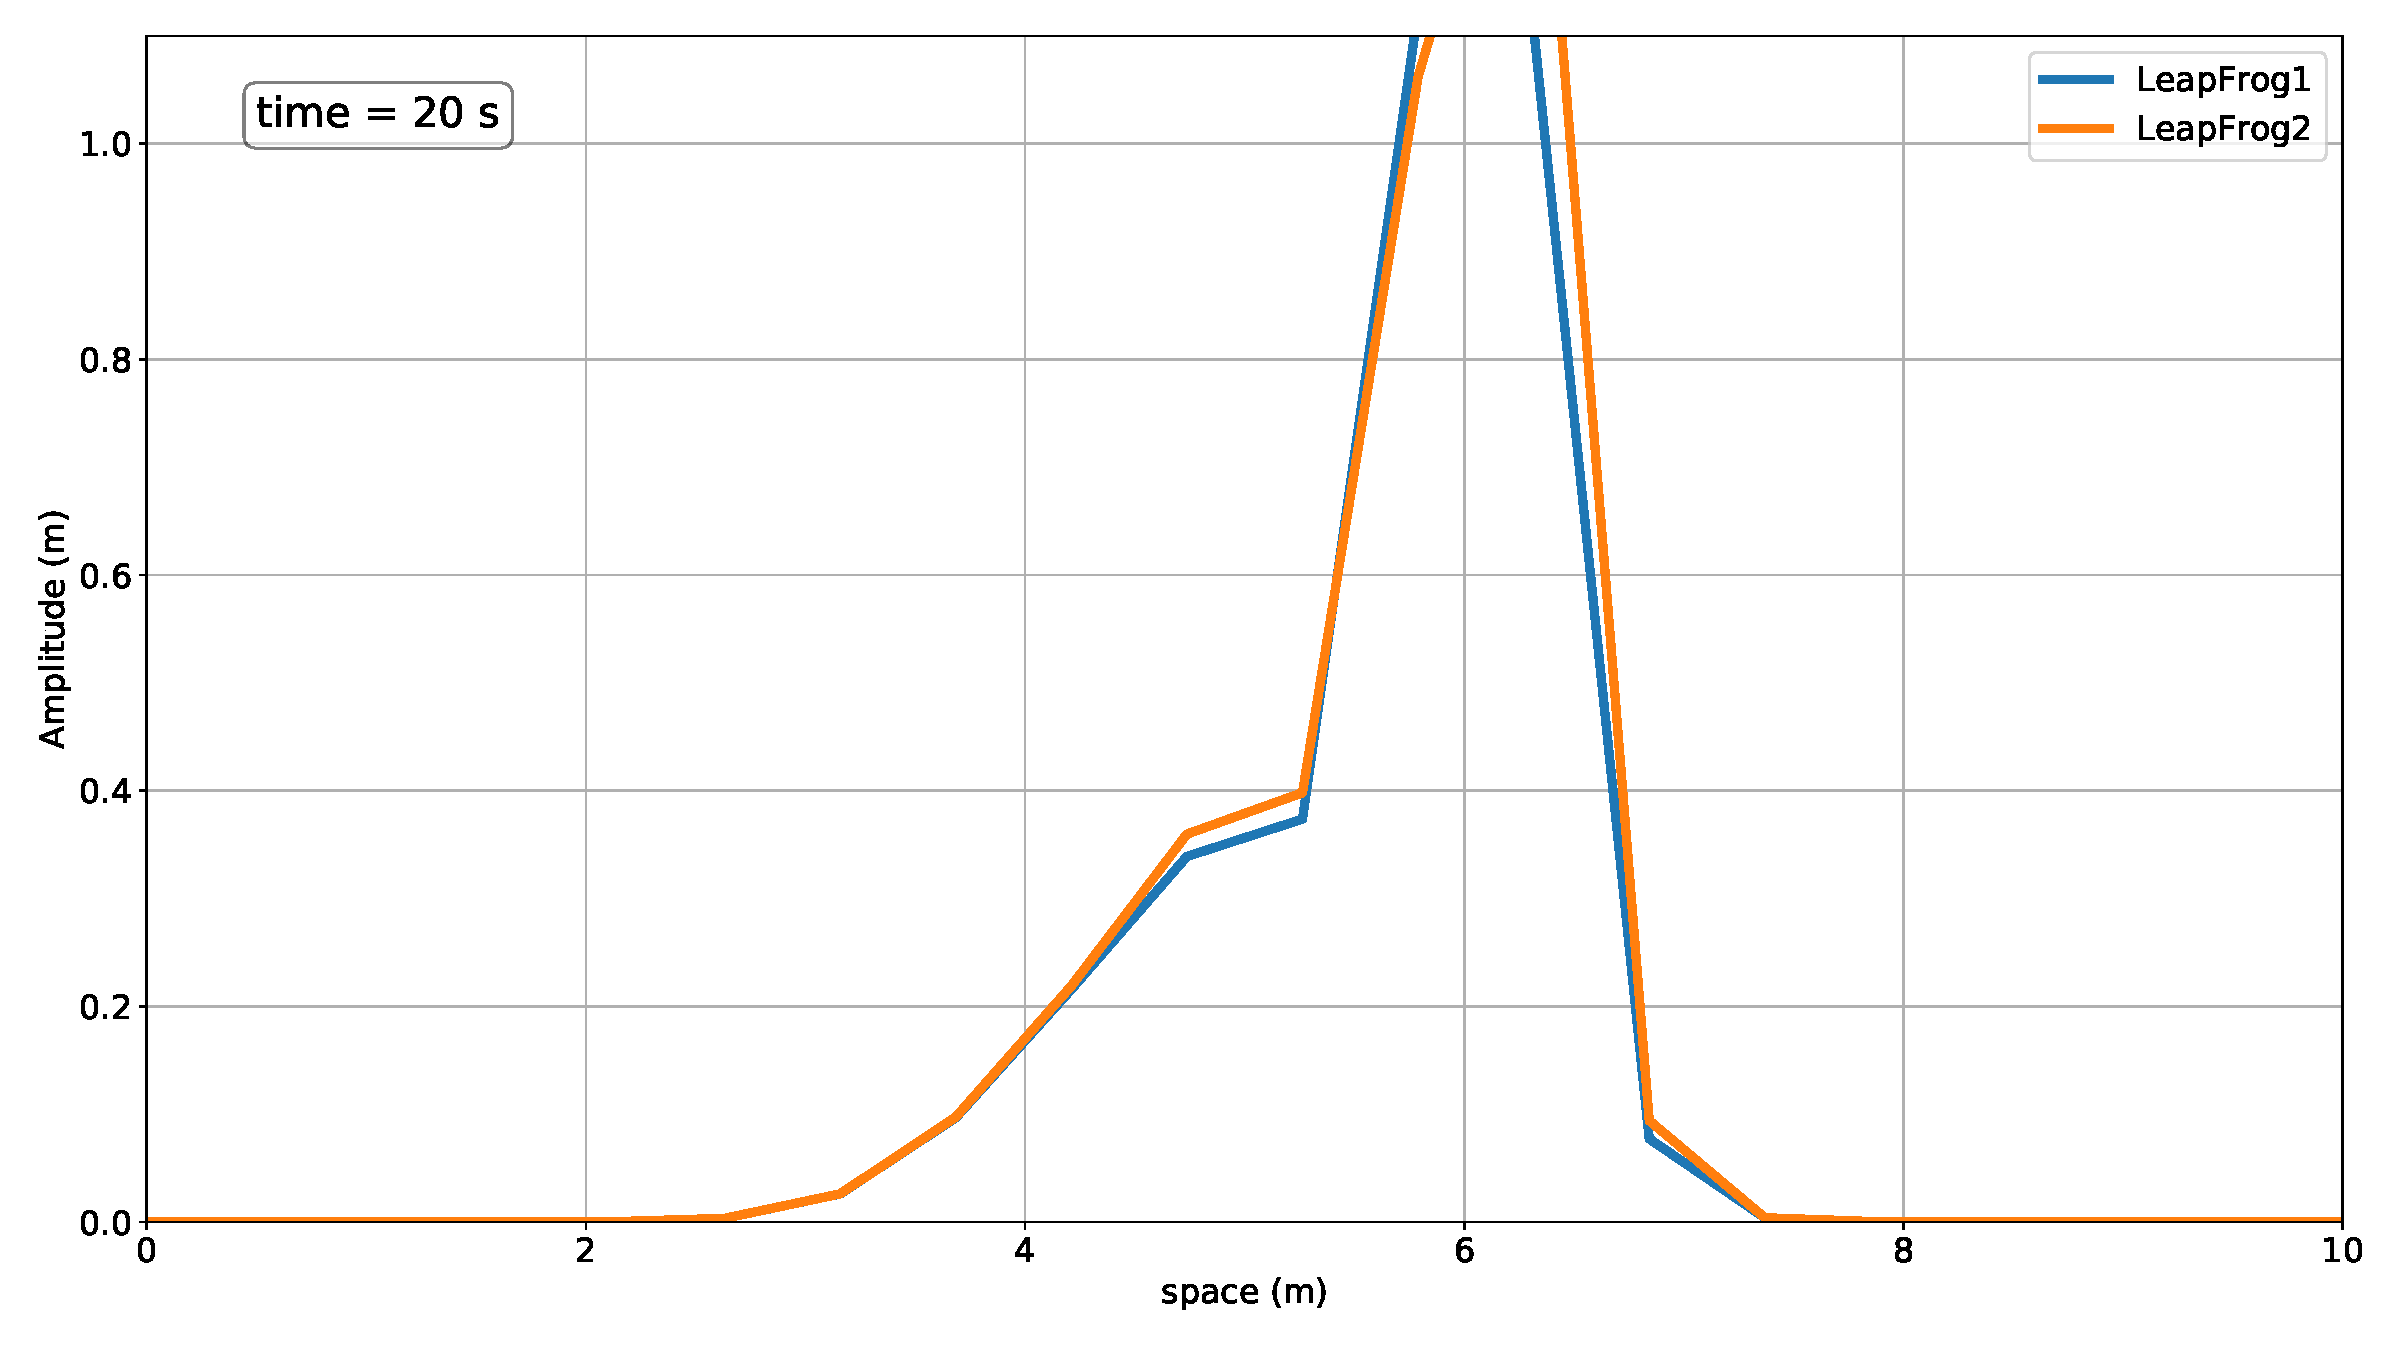
\includegraphics[width=\linewidth]{../BurgersEquation/images/Lin3_Lin44.pdf}
% 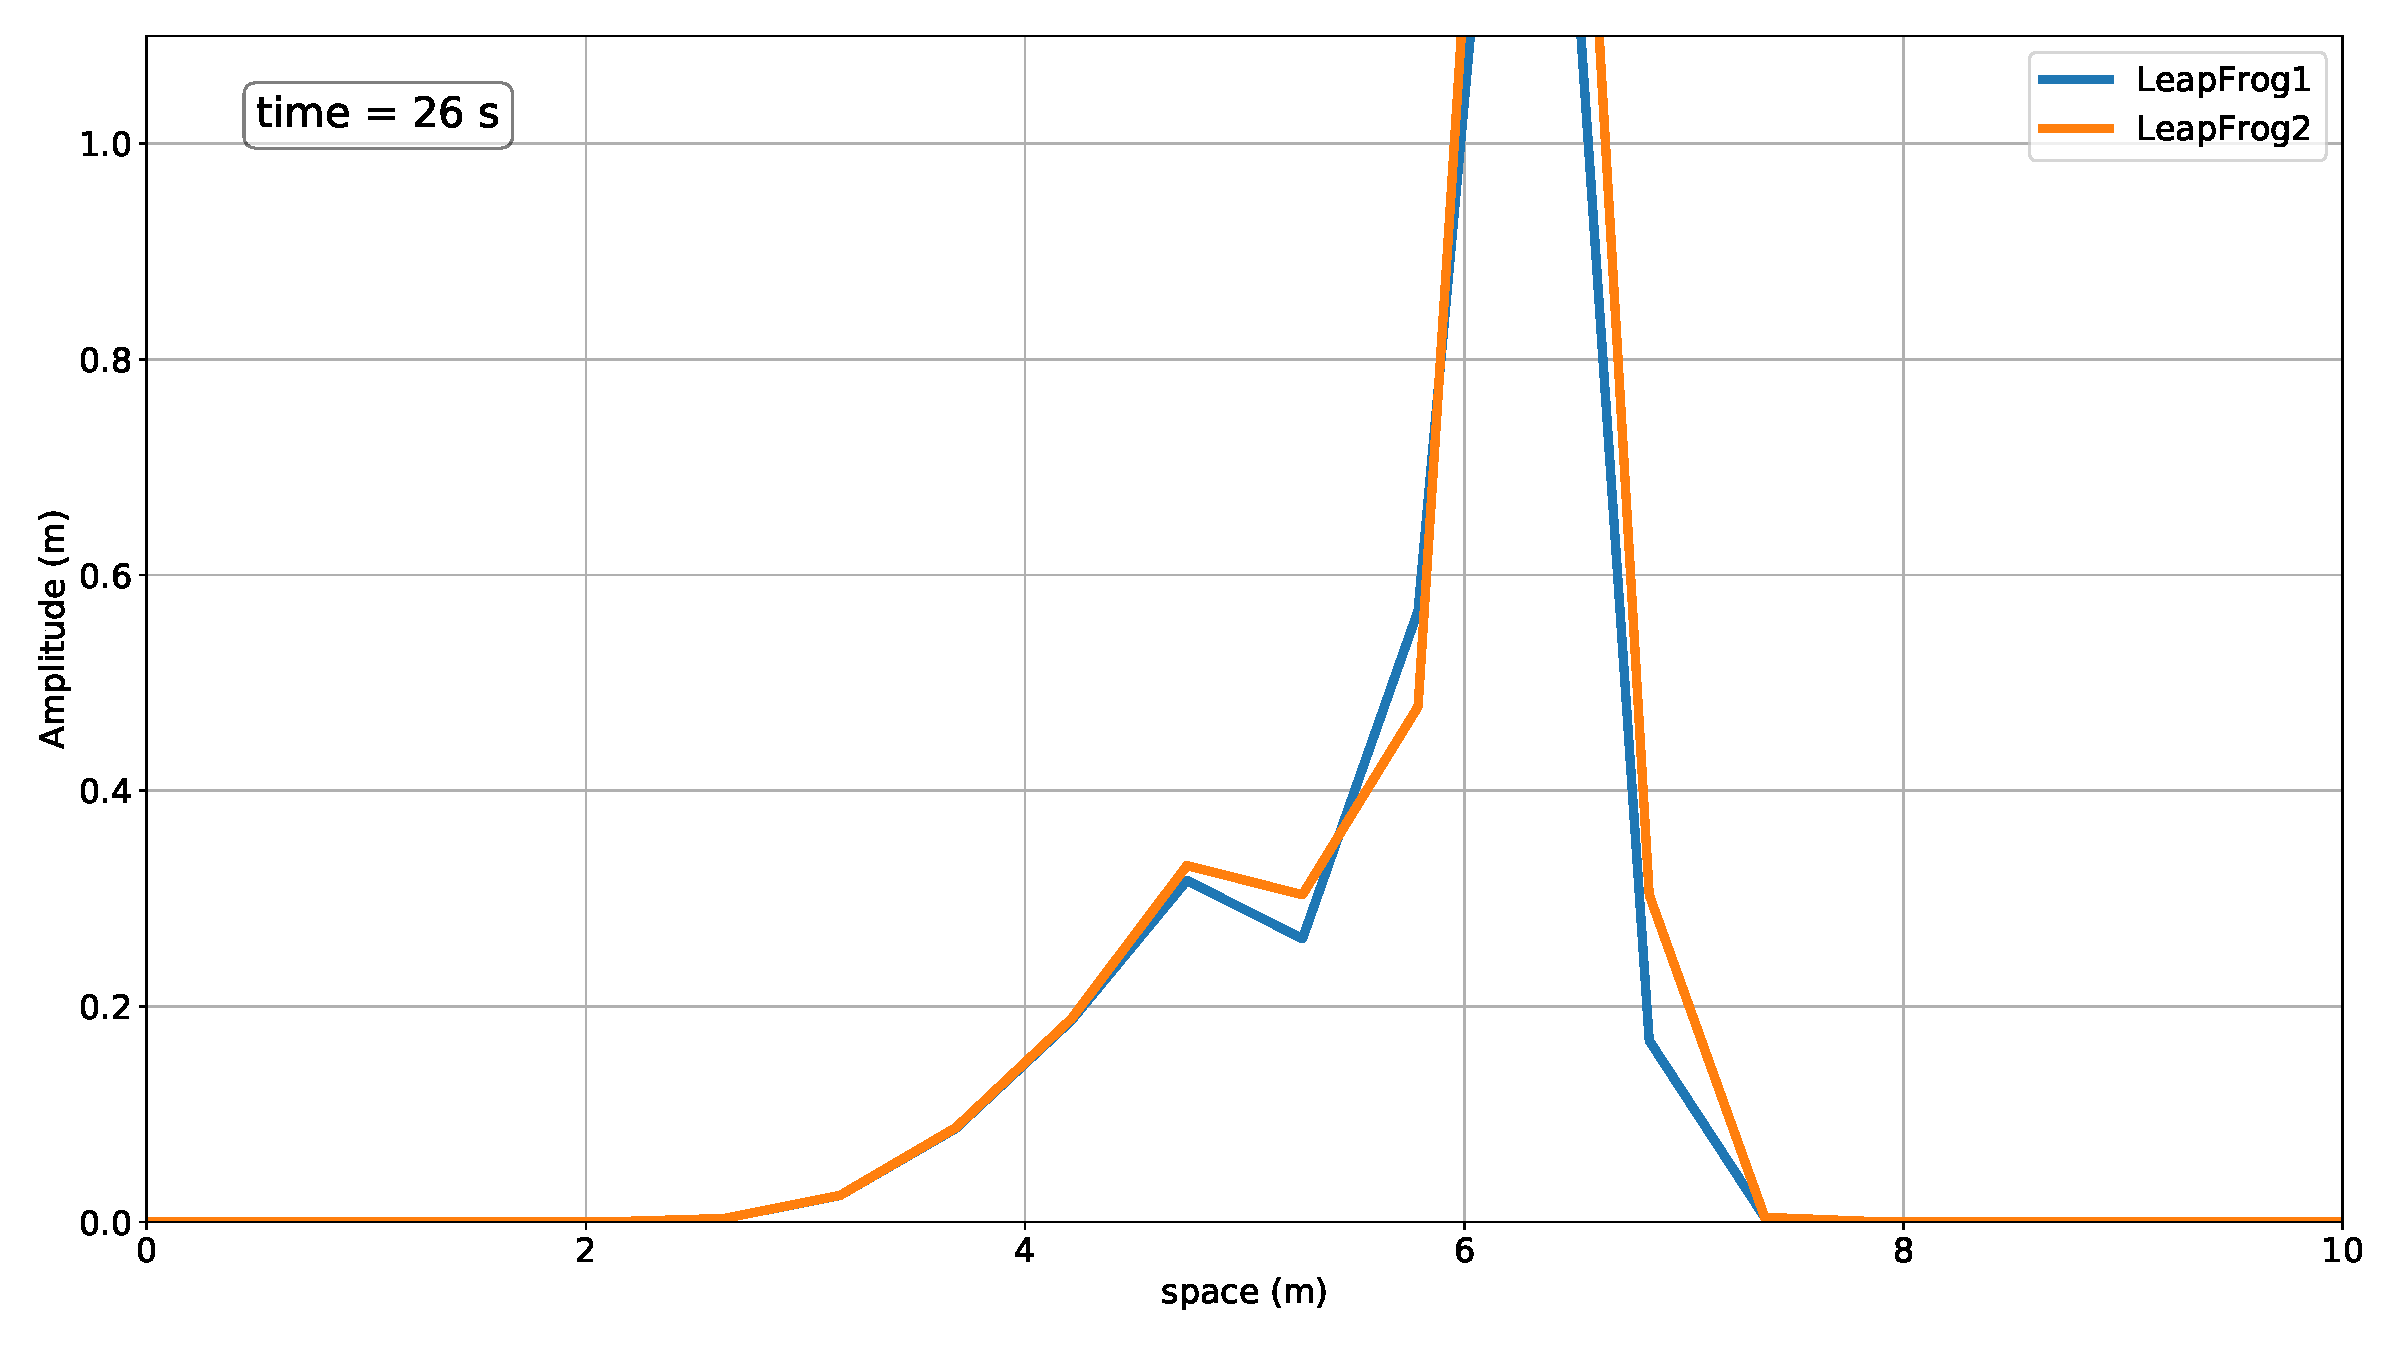
\includegraphics[width=\linewidth]{../BurgersEquation/images/Lin3_Lin45.pdf}
% 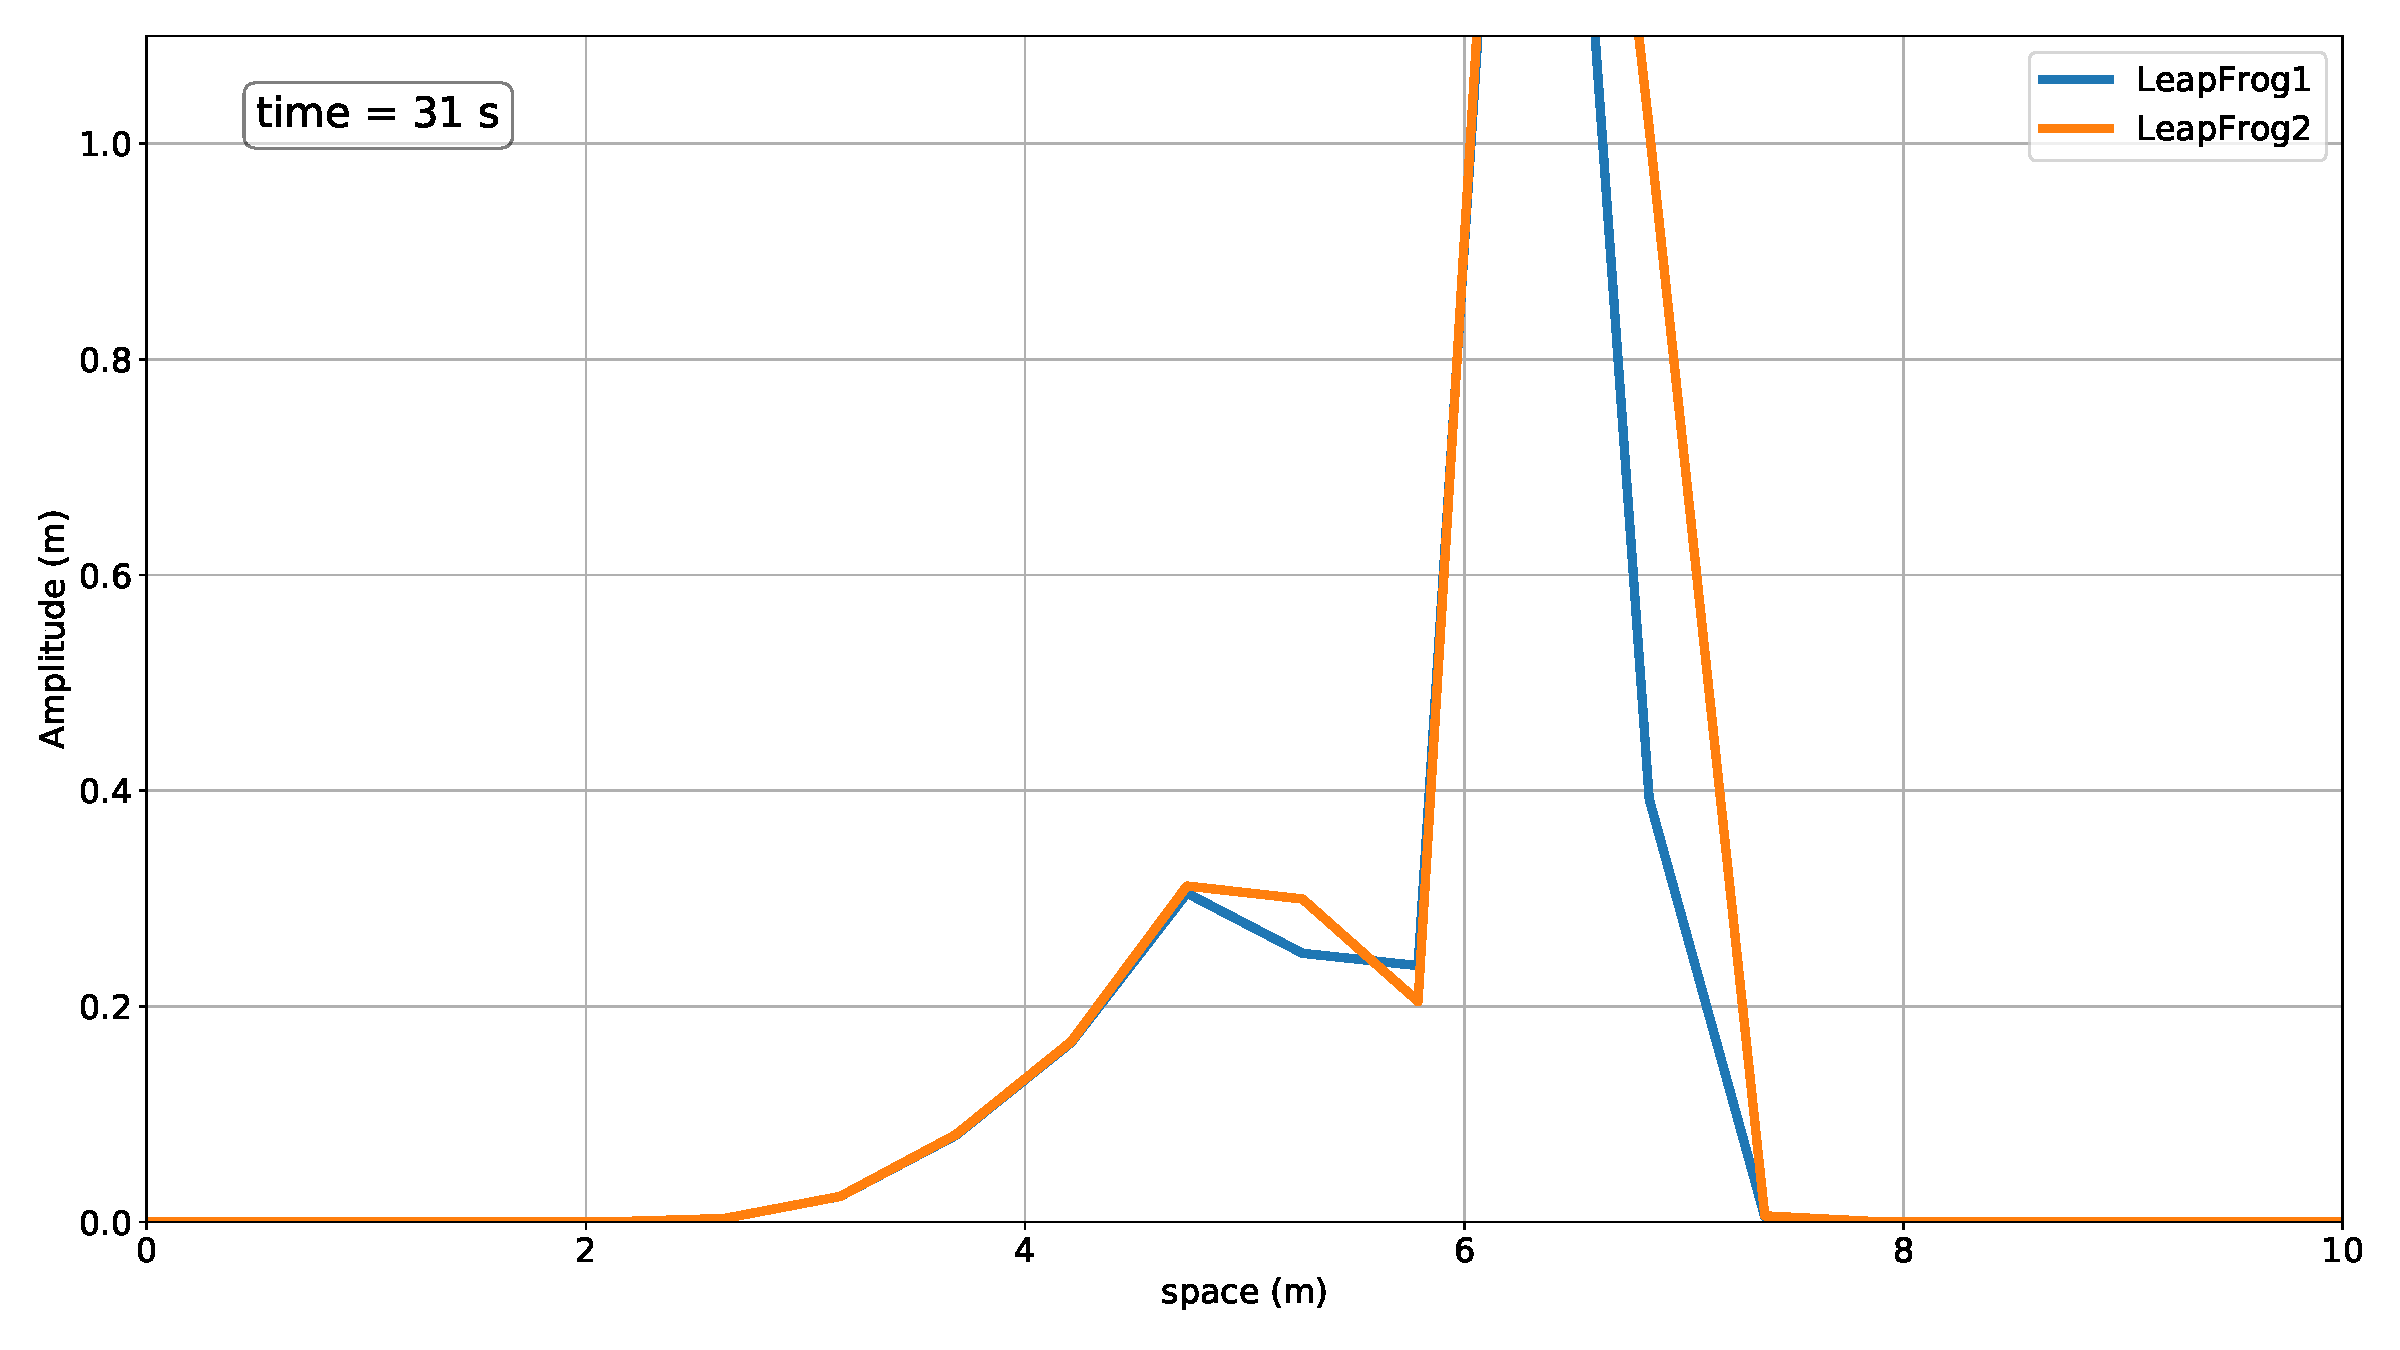
\includegraphics[width=\linewidth]{../BurgersEquation/images/Lin3_Lin46.pdf}
% 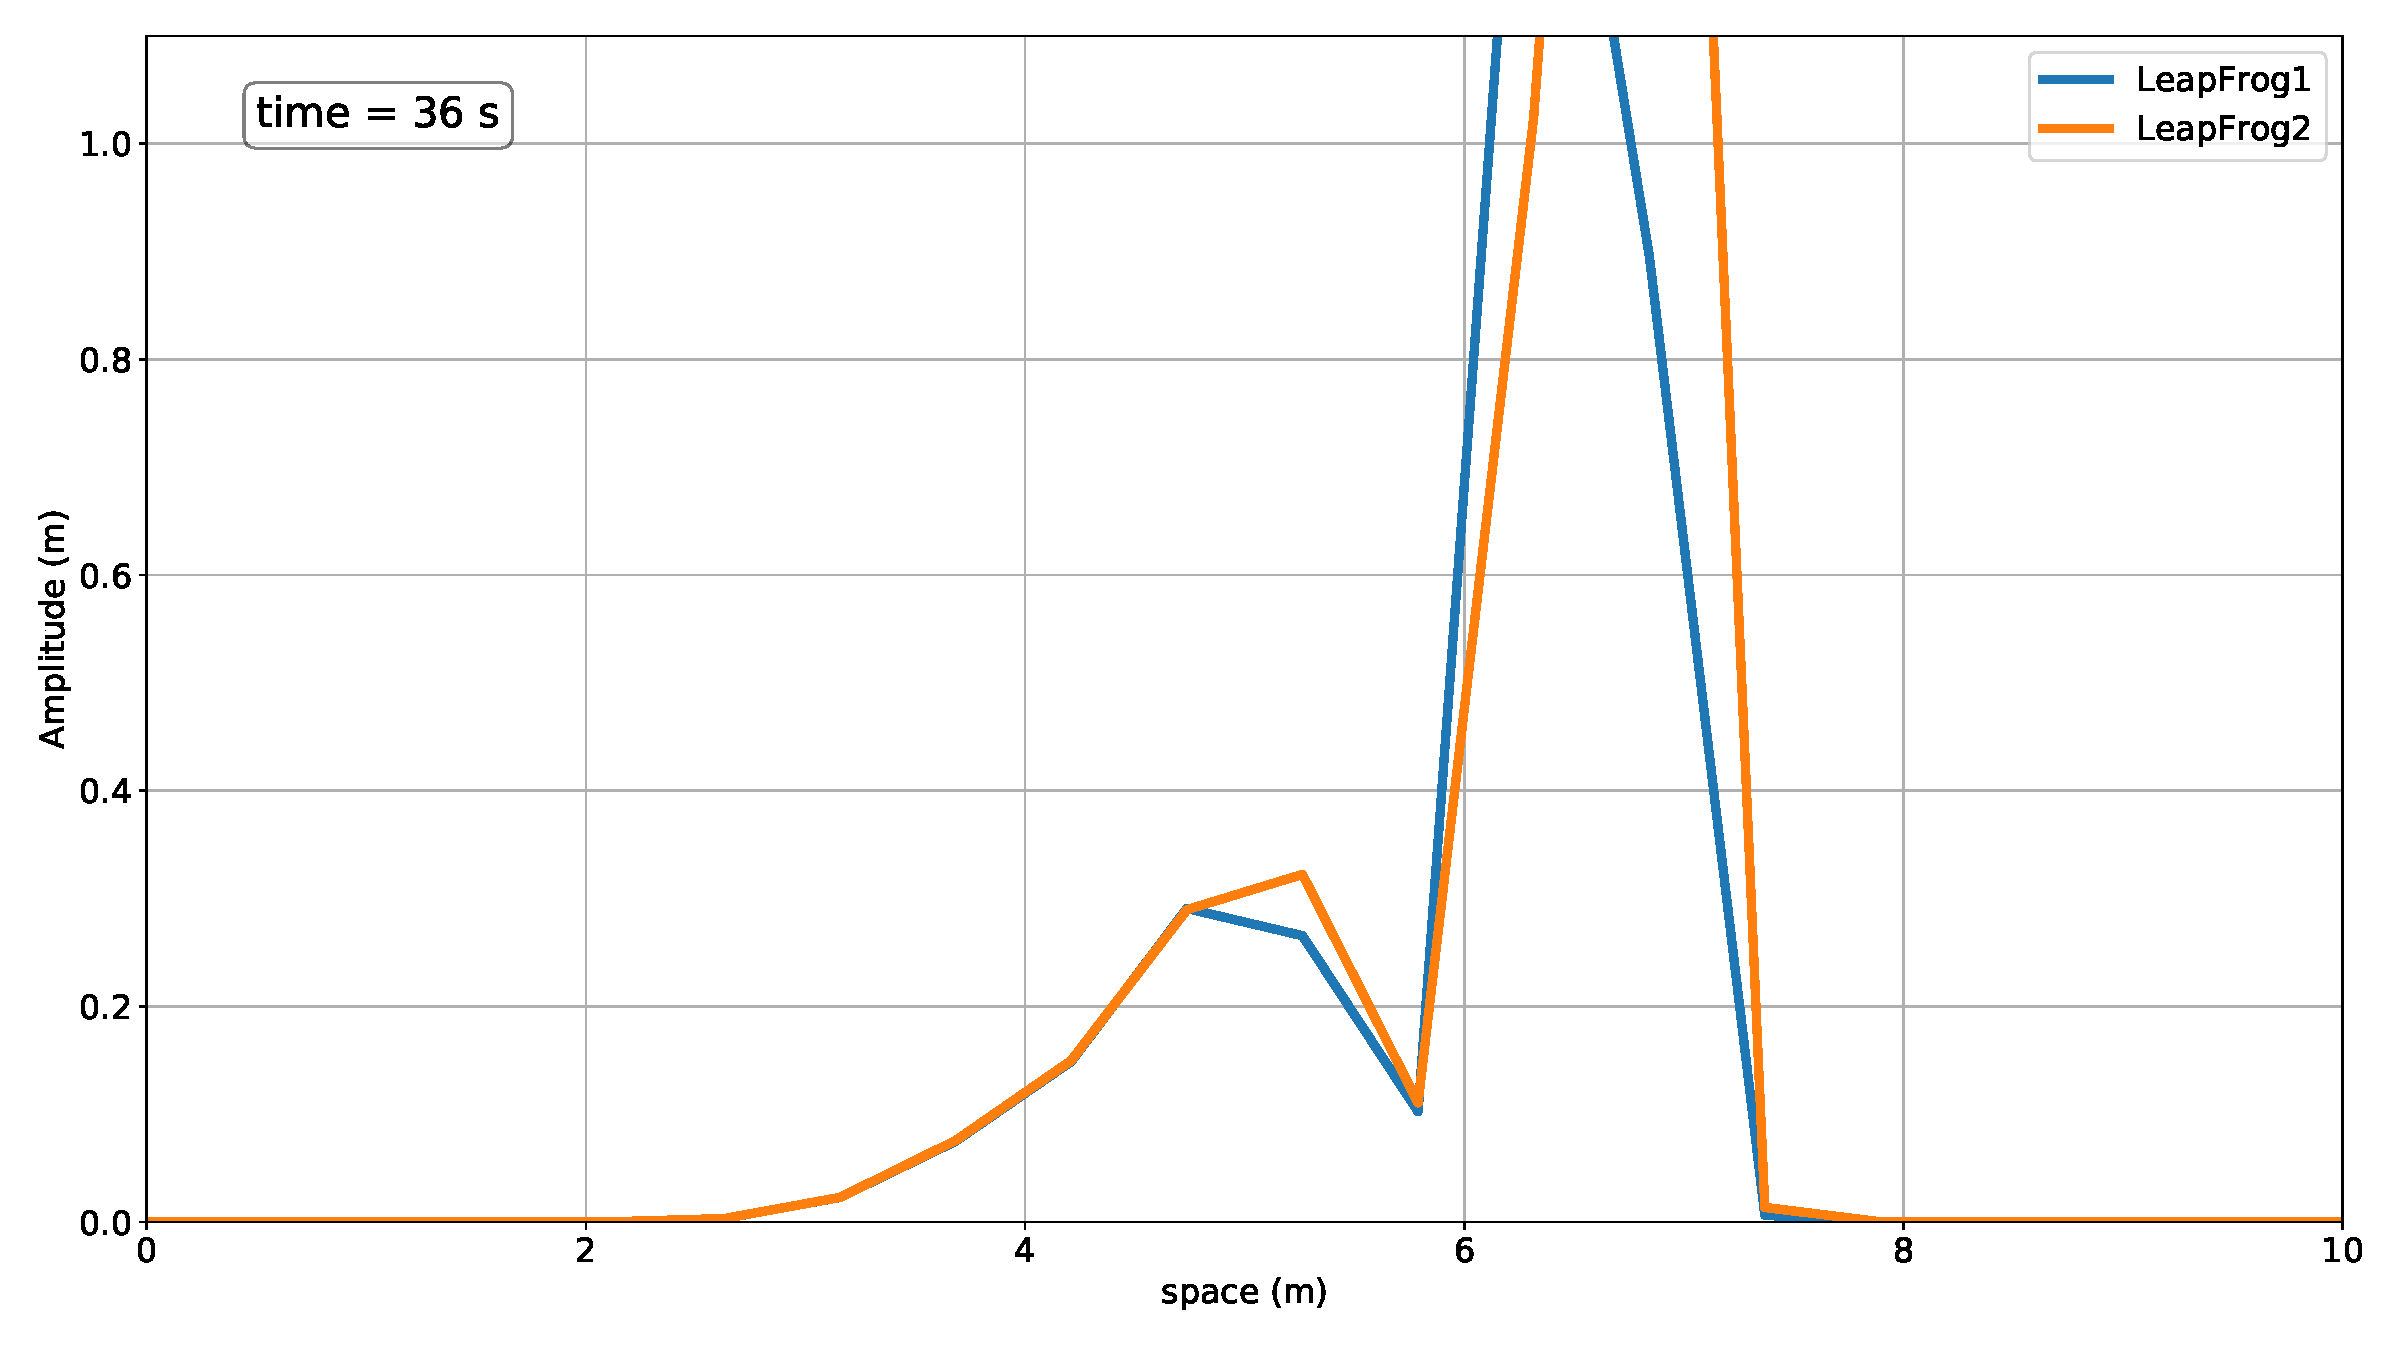
\includegraphics[width=\linewidth]{../BurgersEquation/images/Lin3_Lin47.pdf}
% 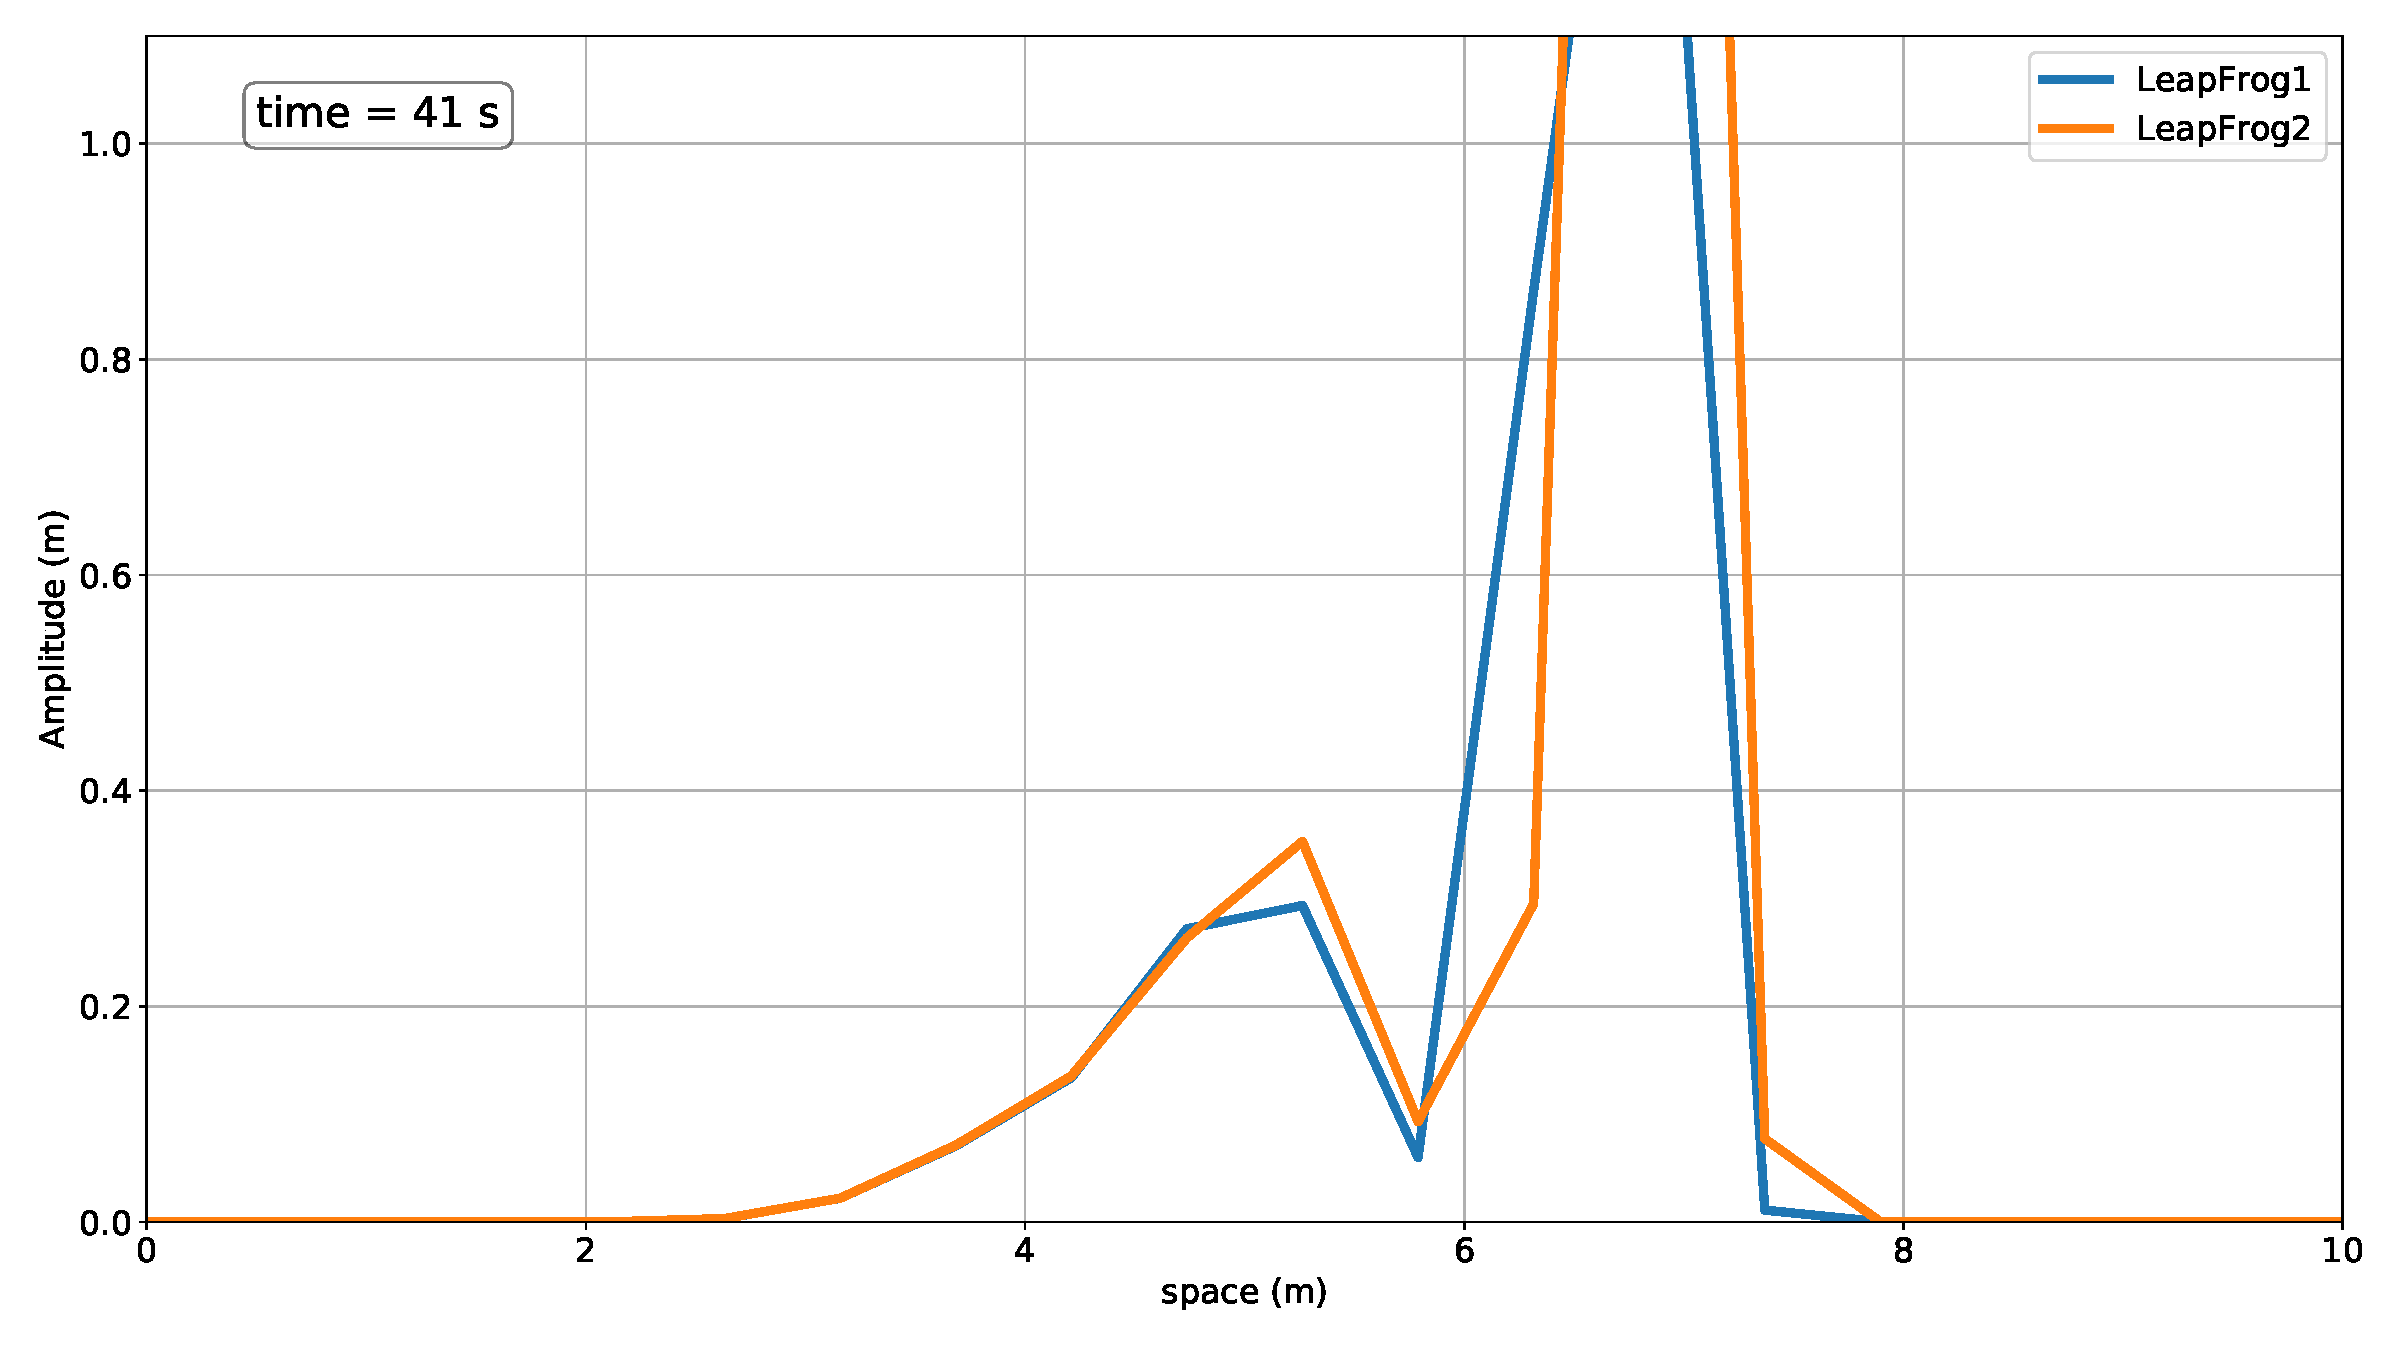
\includegraphics[width=\linewidth]{../BurgersEquation/images/Lin3_Lin48.pdf}
% 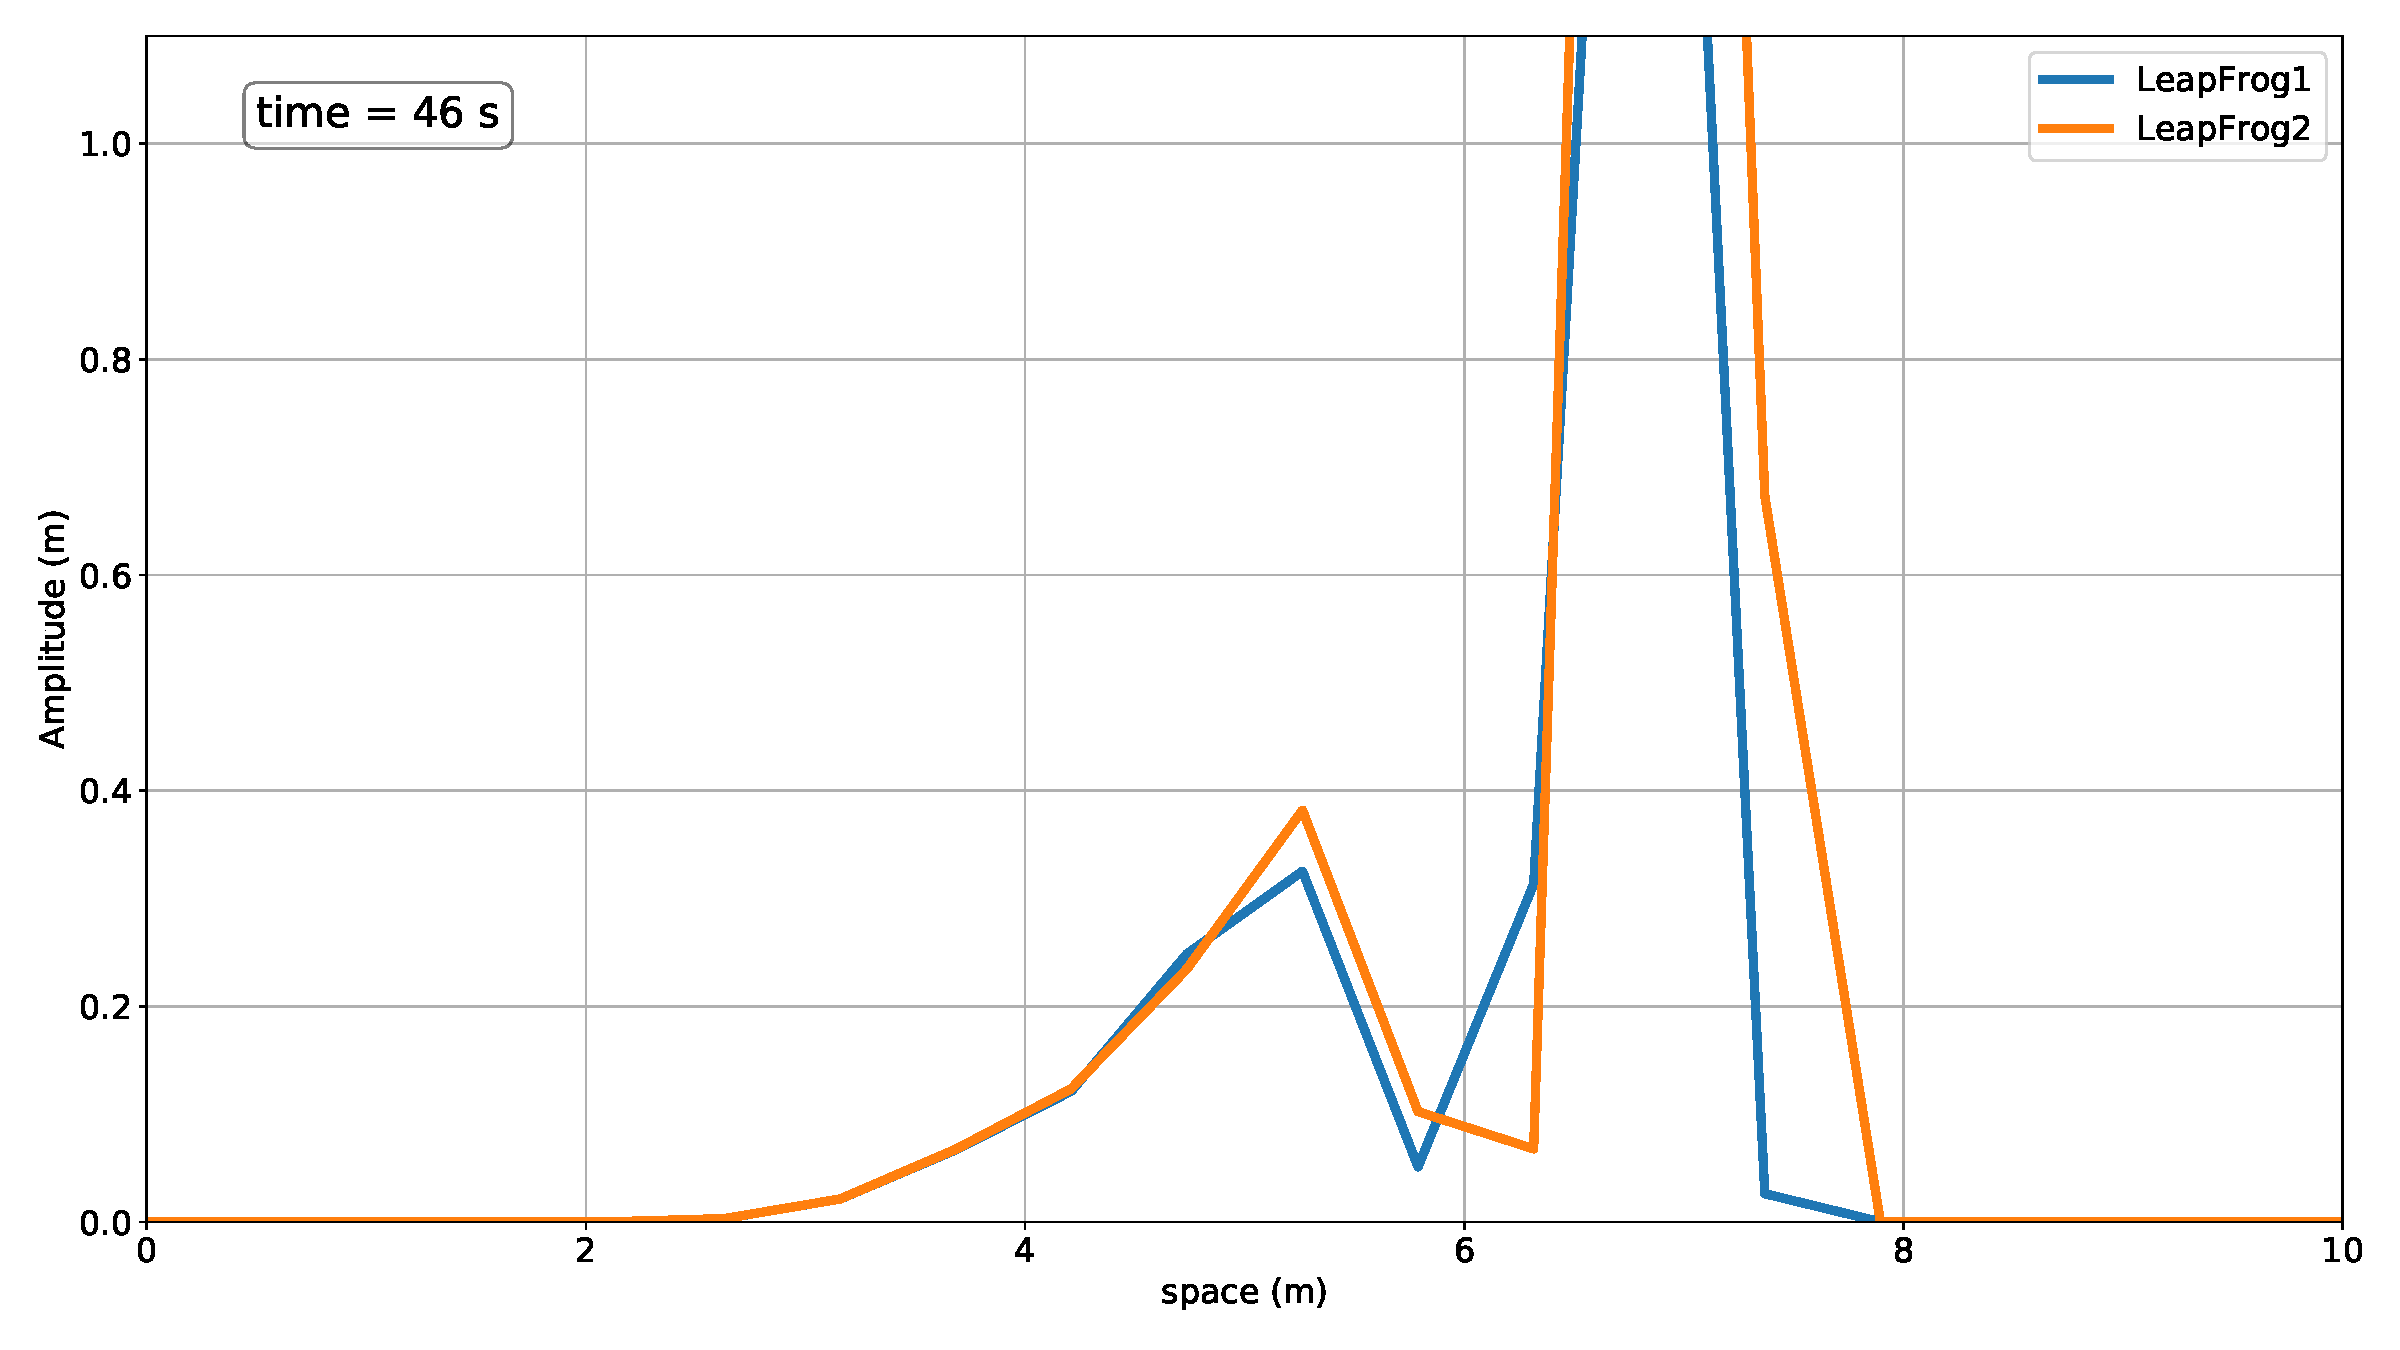
\includegraphics[width=\linewidth]{../BurgersEquation/images/Lin3_Lin49.pdf}

\begin{frame}
  \begin{columns}
    \column{0.5\linewidth}
    \begin{center}
      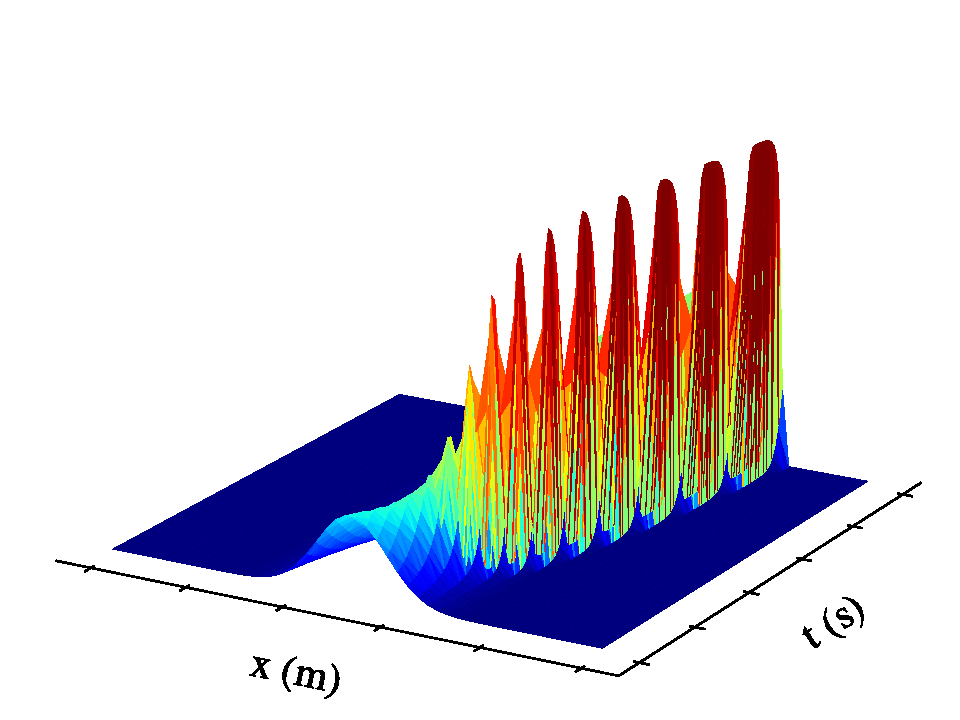
\includegraphics[height=.7\textheight]{../BurgersEquation/images/Leap_Frog_front.pdf}
    \end{center}
    \column{0.5\linewidth}
    \begin{center}
      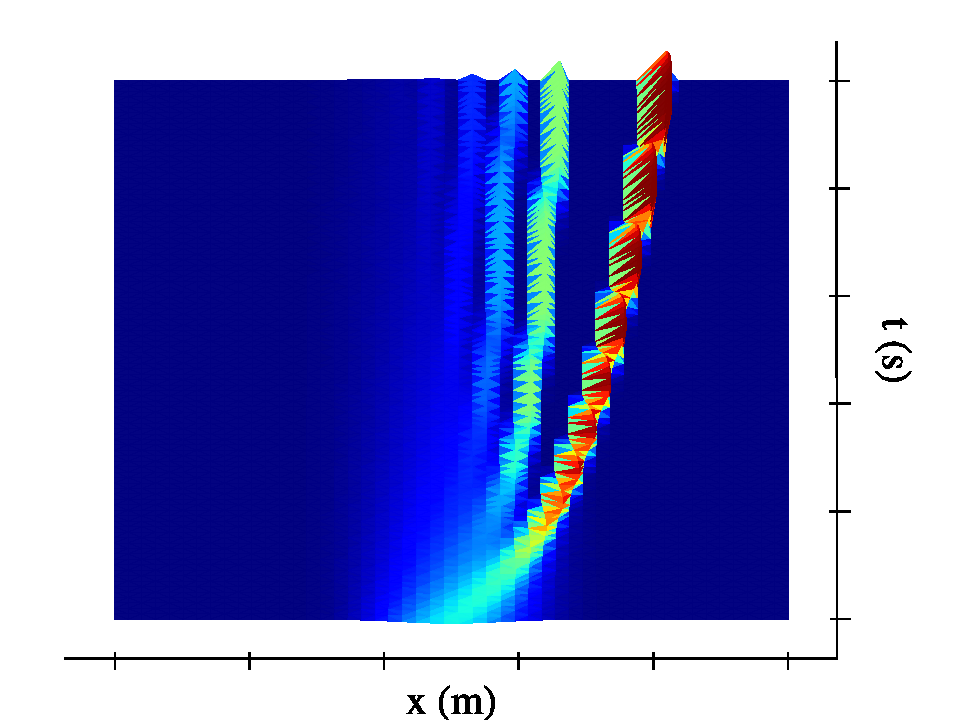
\includegraphics[height=.7\textheight]{../BurgersEquation/images/Leap_Frog_top.pdf}
    \end{center}
  \end{columns}
\end{frame}
